%%%%%%%%%%%%%%%%%%%%%%%%%%%%%%%%%%%%%%%%%%%%%%%%%%%%%%%%%%%%%%%
%
%     filename  = "Tobi-Dissertation.tex",
%     version   = "1.3.0",
%     date      = "2013/10/21",
%     authors   = "Gary L. Gray,
%     copyright = "Gary L. Gray",
%     address   = "Engineering Science and Mechanics,
%                  212 Earth & Engineering Sciences Bldg.,
%                  Penn State University,
%                  University Park, PA 16802,
%                  USA",
%     telephone = "814-863-1778",
%     email     = "gray@psu.edu",
%
%%%%%%%%%%%%%%%%%%%%%%%%%%%%%%%%%%%%%%%%%%%%%%%%%%%%%%%%%%%%%%%
%
% Change History:
%
% 1.3.0	**	Added the cite package.
%
%		**	Give that the Graduate School now allows essentially
%			any line spacing, I have moved the line space setting
%			from psuthesis.cls to this driver file. Go ahead and
%			make it ugly if you want. :-)
%
%		**	Removed \addtocounter{page}{-1} after \psutitlepage is
%			executed. It made the paging of the frontmatter
%			incorrect. I can no longer remember why it was there.
%
%		**	Removed \psusigpage since the Graduate School now
%			provides the signature page.
%
%		**	Added the command \collegesubmittedto to add the College
%			in which the thesis/dissertation has been completed to
%			the title page.
%
%		**	Added instructions for documents that include a single
%			appendix since the Graduate School just hates calling it
%			``Appendix A'' is there is a single appendix.
%
%		**	Removed the fncychap package since I could not easily
%			find a way to make it work with documents that have a
%			single appendix.
%
%		**	Added the titlesec package so that the user can make the
%			format of the chapter titles a little less boring than
%			LaTeX's default.
%
% 1.2.2	**	Added some information to the main driver file (this
%			file) regarding the use of hyperref with the
%			psuthesis class. Thanks to Nathan Urban for pointing
%			out the included workaround.
%
% 1.2.1	**	Finally reproduced and fixed the problem where the
%			page number listed in the TOC for the Bibliography
%			was the last page number of the Bibliography.
%
%		**	Added 10pt and 11pt options to the document class,
%			though we have no idea why anyone would want to use
%			such insanely small font sizes since it will lead to
%			line lengths that are much too long.
%
% 1.2.0	**	Two additional class options have been added to
%			support honors theses submitted to the Schreyer
%			Honors College. These options are:
%			- honors
%			- honorsdepthead
%			See below for details.
%
%		**	We have also added the commands:
%			- honorsdegreeinfo
%			- honorsadviser
%			- honorsdepthead
%			Again, see below for details.
%
% 1.1.2	**	If you want to use the subfigure package with our
%			psuthesis class file, then you must must find the 
%			following line in the psuthesis.cls file:
%
%			\RequirePackage{tocloft}
%
%			and add the subfigure option. We have already set
%			this up for you in the psuthesis.cls file to make
%			this easy to do.
%
% 1.1.1	**	Added the fncychap package to the distribution.
%
% 1.1.0	**	The way that the thesis frontmatter and backmatter
%			is generated has been completely re-done in order
%			to be more intuitive.
%
%		**	We have added the ability to change the title of
%			the Dedication/Epigraph to anything you please.
%
%		**	In the process of changing the format of the Table
%			of Contents to conform to the inflexible rules of
%			the Grad School (the word ``Chapter'' and
%			``Appendix'' need to appear before the number and
%			letter, respectively), we have added an option to
%			the class called inlinechaptertoc that changes the
%			format of the Chapter/Appendix entries in the TOC.
%			Note that the tocloft package is now required.
%
%		**	Appendices should now start with the
%			\Appendix command rather than \chapter. See the
%			accompanying files for examples.
%
%		**	Added information regarding the Nontechnical
%			Abstract that is required of ESM students.
%
%		**	Added the fncychap package for those of you who like
%			the nice Chapter headings it provides. We like
%			Lenny, but you don't have to use it if you don't
%			want to. In addition, the other options are: Sonny,
%			Glenn, Conny, Rejne, and Bjarne
%
% 1.0.4	**	fixed the \addcontentsline entry for BibTeX within
%			the commented out text in the Bibliography section
%
% 1.0.3	**	added a sigpage option to conform to new Grad School
%			requirements
%
% 1.0.2	**	issued the \appendix command to start the appendices
%
%		**	moved the \addcontentsline for the bibliography so
%			that the bibliography now shows up on the right page
%			in the TOC
%
%		**	added some info if you use bibtex
%
% 1.0.1	**	eqlist and eqparbox are now included in the archive
%
%%%%%%%%%%%%%%%%%%%%%%%%%%%%%%%%%%%%%%%%%%%%%%%%%%%%%%%%%%%%%%%
%
% This is a template file to help get you started using the
% psuthesis.cls for theses and dissertations at Penn State
% University. You will, of course, need to put the
% psuthesis.cls file someplace that LaTeX will find it.
%
% We have set up a directory structure that we find to be clean
% and convenient. You can readjust it to suit your tastes. In
% fact, the structure used by our students is even a little
% more involved and commands are defined to point to the
% various directories.
%
% This document has been set up to be typeset using pdflatex.
% About the only thing you will need to change if typesetting
% using latex is the \DeclareGraphicsExtensions command.
%
% The psuthesis document class uses the same options as the
% book class. In addition, it requires that you have the
% ifthen, calc, setspace, and tocloft packages.
%
% The first additional option specifies the degree type. You
% can choose from:
%	Ph.D. using class option <phd>
%	M.S. using class option <ms>
%	M.Eng. using class option <meng>
%	M.A. using class option <ma>
%	B.S. using class option <bs>
%	B.A. using class option <ba>
%	Honors Baccalaureate using the option <honors>
%
% If you specify either ba or bs in addition to honors, it will
% just use the honors option and ignore the ba or bs option.
%
% The second additional option <inlinechaptertoc> determines
% the formatting of the Chapter entries in the Table of
% Contents. The default sets them as two-line entries (try it).
% If you want them as one-line entries, issue the
% inlinechaptertoc option.
%
% The class option ``honors'' should be used for theses
% submitted to the Schreyer Honors College. This option
% changes the formatting on the Title page so that the
% signatures appear on the Title page.
%
% The class option ``honorsdepthead'' adds the signature of the
% department head on the Title page for those baccalaureate
% theses that require this.
%
% The class option ``secondthesissupervisor'' should be used
% for baccalaureate honors degrees if you have a second
% Thesis Supervisor.
%
% The vita is only included with the phd option and it is
% placed at the end of the thesis. The permissions page is only
% included with the ms, meng, and ma options.
%%%%%%%%%%%%%%%%%%%%%%%%%%%%%%%%%%%%%%%%%%%%%%%%%%%%%%%%%%%%%%%
% Only one of the following lines should be used at a time.
%\documentclass[draft,phd,12pt]{psuthesis}
%\documentclass[draft,phd,inlinechaptertoc]{psuthesis}
%\documentclass[draft,ms]{psuthesis}
%\documentclass[draft,honorsdepthead,honors]{psuthesis}
\documentclass[phd,12pt]{psuthesis}

\usepackage[T1]{fontenc}
\usepackage{lmodern}
\usepackage{textcomp}
\usepackage{microtype}

%%%%%%%%%%%%%%%%%%%%%%%%%%%%
% Packages we like to use. %
%%%%%%%%%%%%%%%%%%%%%%%%%%%%
\usepackage{amsmath}
\usepackage{amssymb}
\usepackage{amsthm}
\usepackage{exscale}
\usepackage[mathscr]{eucal}
\usepackage{bm}
\usepackage{eqlist} % Makes for a nice list of symbols.
\usepackage[final]{graphicx}
\usepackage[dvipsnames]{color}
\DeclareGraphicsExtensions{.pdf, .jpg}
\usepackage{float}
\usepackage{gensymb}
\usepackage{wasysym}
% http://www.tex.ac.uk/cgi-bin/texfaq2html?label=citesort
\usepackage{cite}

\usepackage{titlesec}
\usepackage{multirow}

%%%%%%%%%%%%%%%%%%%%%%%%%%%%%%%
% Use of the hyperref package %
%%%%%%%%%%%%%%%%%%%%%%%%%%%%%%%
%
% This is optional and is included only for those students
% who want to use it.
%
% To the hyperref package, uncomment the following line:
\usepackage{hyperref}
%
% Note that you should also uncomment the following line:
%\renewcommand{\theHchapter}{\thepart.\thechapter}
%
% to work around some a problem hyperref has with the fact
% the psuthesis class has unnumbered pages after which page
% counters are reset.

% Set the baselinestretch using the setspace package.
% The LaTeX Companion claims that a \baselinestretch of
% 1.24 gives one-and-a-half line spacing, which is allowed
% by the PSU thesis office. As of October 18, 2013, the Graduate
% School states ``The text of an eTD may be single-, double- or
% one- and-a-half-spaced.'' Go nuts!
\setstretch{1.24}


%%%%%%%%%%%%%%%%%%%%%%%%%%%%%%%%%%%%
% SPECIAL SYMBOLS AND NEW COMMANDS %
%%%%%%%%%%%%%%%%%%%%%%%%%%%%%%%%%%%%
% Place user-defined commands below.



%%%%%%%%%%%%%%%%%%%%%%%%%%%%%%%%%%%%%%%%%
% Renewed Float Parameters              %
% (Makes floats fit better on the page) %
%%%%%%%%%%%%%%%%%%%%%%%%%%%%%%%%%%%%%%%%%
\renewcommand{\floatpagefraction}{0.85}
\renewcommand{\topfraction}      {0.85}
\renewcommand{\bottomfraction}   {0.85}
\renewcommand{\textfraction}     {0.15}

% ----------------------------------------------------------- %

%%%%%%%%%%%%%%%%
% FRONT-MATTER %
%%%%%%%%%%%%%%%%
% Title
\title{Mechanisms of Sintering and Second Phase Formation in Bayer Alumina}

% Author and Department
\author{Tobias Frueh}
\dept{Materials Science and Engineering}
% the degree will be conferred on this date
\degreedate{September 2017}
% year of your copyright
\copyrightyear{2017}

% This command is used for students submitting a thesis to the
% Schreyer Honors College. The argument of this command should
% contain every after the word ``requirements'' that appears on
% the title page. This provides the needed flexibility for
% all the degree types.
%\honorsdegreeinfo{for a baccalaureate degree \\ in Engineering Science \\ with honors in Engineering Science}

% This is the document type. For example, this could also be:
%	Comprehensive Document
%	Thesis Proposal
%\documenttype{Thesis}
\documenttype{Dissertation}
%\documenttype{Comprehensive Document}


% This will generally be The Graduate School, though you can
% put anything in here to suit your needs.
\submittedto{The Graduate School}

% This is the college to in which you are submitting the
% thesis/dissertation.
\collegesubmittedto{College of Earth and Mineral Sciences}


%%%%%%%%%%%%%%%%%%
% Signatory Page %
%%%%%%%%%%%%%%%%%%
% You can have up to 7 committee members, i.e., one advisor
% and up to 6 readers.
%
% Begin by specifying the number of readers.
\numberofreaders{3}

% For baccalaureate honors degrees, enter the name of your
% honors adviser below.
%\honorsadviser{Honors P. Adviser}

% For baccalaureate honors degrees, if you have a second
% Thesis Supervisor, enter his or her name below.
%\secondthesissupervisor{Second T. Supervisor}

% For baccalaureate honors degrees, certain departments
% (e.g., Engineering Science and Mechanics) require the
% signature of the department head. In that case, enter the
% name of your department head below.
%\honorsdepthead{Department Q. Head}

% Input reader information below. The optional argument, which
% comes first, goes on the second line before the name.
\advisor[Dissertation Advisor, Chair of Committee]
		{Gary L. Messing}
		{Distinguished Professor of Ceramic Science and Engineering}

\readerone[]
			{James H. Adair}
			{Professor of Materials Science and Engineering, Biomedical Engineering and Pharmacology}

\readertwo[Associate Dean for Graduate Education and Research]
			{John R. Hellmann}
			{Professor of Materials Science and Engineering}

\readerthree[Department Head, Advanced Coatings at the Applied Research Laboratory Senior Scientist]
			{Dogulas E. Wolfe}
			{Associate Professor of Materials Science and Engineering}

\readerfour[Special Member]
			{Charles E. Compson}
			{Global Technical Director, CPO \newline Almatis, Inc.}

%\readerfive[Optional Title Here]
			%{Reader Name}
			%{Professor of SomeThing}

% Format the Chapter headings using the titlesec package.
% You can format section headings and the like here too.
\definecolor{gray75}{gray}{0.75}
\newcommand{\hsp}{\hspace{15pt}}
\titleformat{\chapter}[display]{\fontsize{30}{30}\selectfont\bfseries\sffamily}{Chapter \thechapter\hsp\textcolor{gray75}{\raisebox{3pt}{|}}}{0pt}{}{}

\titleformat{\section}[block]{\Large\bfseries\sffamily}{\thesection}{12pt}{}{}
\titleformat{\subsection}[block]{\large\bfseries\sffamily}{\thesubsection}{12pt}{}{}


% Makes use of LaTeX's include facility. Add as many chapters
% and appendices as you like.
\includeonly{%
Chapter-1/Chapter-1,%
Chapter-2/Chapter-2,%
Chapter-3/Chapter-3,%
Chapter-4/Chapter-4,%
Chapter-5/Chapter-5,%
Chapter-6/Chapter-6,%
Chapter-7/Chapter-7%
}

\usepackage{listings}
%%%%%%%%%%%%%%%%%
% THE BEGINNING %
%%%%%%%%%%%%%%%%%
\begin{document}
%%%%%%%%%%%%%%%%%%%%%%%%
% Preliminary Material %
%%%%%%%%%%%%%%%%%%%%%%%%
% This command is needed to properly set up the frontmatter.
\frontmatter

%%%%%%%%%%%%%%%%%%%%%%%%%%%%%%%%%%%%%%%%%%%%%%%%%%%%%%%%%%%%%%
% IMPORTANT
%
% The following commands allow you to include all the
% frontmatter in your thesis. If you don't need one or more of
% these items, you can comment it out. Most of these items are
% actually required by the Grad School -- see the Thesis Guide
% for details regarding what is and what is not required for
% your particular degree.
%%%%%%%%%%%%%%%%%%%%%%%%%%%%%%%%%%%%%%%%%%%%%%%%%%%%%%%%%%%%%%
% !!! DO NOT CHANGE THE SEQUENCE OF THESE ITEMS !!!
%%%%%%%%%%%%%%%%%%%%%%%%%%%%%%%%%%%%%%%%%%%%%%%%%%%%%%%%%%%%%%

% Generates the title page based on info you have provided
% above.
\psutitlepage

% Generates the committee page -- this is bound with your
% thesis. If this is an baccalaureate honors thesis, then
% comment out this line.
\psucommitteepage

% Generates the abstract. The argument should point to the
% file containing your abstract. 
\thesisabstract{SupplementaryMaterial/Abstract}

% Generates the Table of Contents
\thesistableofcontents

% Generates the List of Figures
\thesislistoffigures

% Generates the List of Tables
\thesislistoftables

% Generates the List of Symbols. The argument should point to
% the file containing your List of Symbols. 
%\thesislistofsymbols{SupplementaryMaterial/ListOfSymbols}

% Generates the Acknowledgments. The argument should point to
% the file containing your Acknowledgments. 
\thesisacknowledgments{SupplementaryMaterial/Acknowledgments}

% Generates the Epigraph/Dedication. The first argument should
% point to the file containing your Epigraph/Dedication and
% the second argument should be the title of this page. 
\thesisdedication{SupplementaryMaterial/Dedication}{Dedication}



%%%%%%%%%%%%%%%%%%%%%%%%%%%%%%%%%%%%%%%%%%%%%%%%%%%%%%
% This command is needed to get the main part of the %
% document going.                                    %
%%%%%%%%%%%%%%%%%%%%%%%%%%%%%%%%%%%%%%%%%%%%%%%%%%%%%%
\thesismainmatter

%%%%%%%%%%%%%%%%%%%%%%%%%%%%%%%%%%%%%%%%%%%%%%%%%%
% This is an AMS-LaTeX command to allow breaking %
% of displayed equations across pages. Note the  %
% closing the "}" just before the bibliography.  %
%%%%%%%%%%%%%%%%%%%%%%%%%%%%%%%%%%%%%%%%%%%%%%%%%%
\allowdisplaybreaks{
%\pagestyle{fancy}
%\fancyhead{}
%
%%%%%%%%%%%%%%%%%%%%%%
% THE ACTUAL CONTENT %
%%%%%%%%%%%%%%%%%%%%%%
% Chapters
%SourceDoc ../YourName-Dissertation.tex
\vspace*{-80mm}
\chapter{Statement of Problem} \label{chapter1:introduction}

\section{section1.1}
Pestorius [200] developed an algorithm to investigate propagation of finite-am\-pli\-tude noise in pipes. His algorithm, based on weak shock theory, includes the effects of nonlinearity and tube wall boundary layer attenuation and dispersion. The hybrid time-frequency domain algorithm applies nonlinearity in the time domain, applies a fast Fourier transform (FFT), and then applies attenuation and dispersion in the frequency domain.  Then an inverse FFT is taken to return to the time domain to propagate to the next step.

\subsection{subsection1.1.1}


\chapter{The Effects of Na$_{2}$O and SiO$_{2}$ on Liquid Phase Sintering of Bayer Al$_{2}$O$_{3}$}

\section{Introduction}
Al$_{2}$O$_{3}$ is arguably the most extensively used and researched ceramic material because it is used in many large volume applications such as high temperature refractories, technical ceramics, high voltage insulators, and functional fillers. The majority of Al$_{2}$O$_{3}$ applications use synthetic or specialty aluminas derived from Bayer feedstocks, such as aluminum trihydrate (Al(OH)$_{3}$), smelter grade Al$_{2}$O$_{3}$ and others. Bayer process aluminas are typically 99.0 - 99.9\% pure and contain Na$_{2}$O, CaO, Fe$_{2}$O$_{3}$, and SiO$_{2}$ impurities that originate from the bauxite ore and/or Bayer process reagents (e.g., NaOH). The vast majority of research on the sintering of Al$_{2}$O$_{3}$, however, focuses on ultra-high purity ($\geq$ 99.99\%) aluminas derived from specialty feedstocks, such as ammonium alum (NH$_{4}$Al(SO$_{4}$)$_{2}$$\cdot$12H$_{2}$O), boehmite ($\gamma$-AlOOH) and aluminum chloride (AlCl$_{3}$). While ultra-high purity aluminas provide the purest platform from which to conduct fundamental sintering research, that research does not usually explore the types and amounts of impurities typical of Bayer aluminas.  Commercial Bayer Al$_{2}$O$_{3}$ powders exist in a range of reactive grades that differ in the amount and types of these impurities. Therefore, the evaluation of specialty reactive aluminas, within the context of previous work on ultra-high purity aluminas, is a valuable contribution to industrial users and bridges fundamental sintering research with ultra-high purity aluminas.

\section{Experimental}

A chemically purified 0.4 $\mu$m median particle size Bayer process Al$_{2}$O$_{3}$ powder (Almatis, Inc., Leetsdale, PA, USA) with only 2 ppm MgO was used to study the sintering of near MgO-free Bayer Al$_{2}$O$_{3}$ (Figure \ref{Ch2-figure:Figure1}). The powder was chemically purified by the manufacturer so that impurity levels similar to commercial high purity Bayer process aluminas were obtained after doping with Na$_{2}$O and/or SiO$_{2}$. The physical and chemical characteristics of the as-received powder are shown in Table \ref{Ch2-table:table1}. Chemical analysis of the as-received Al$_{2}$O$_{3}$ was performed by inductively coupled plasma (ICP) emission spectroscopy (iCap 6000, Thermo Fischer Scientific, Inc., Waltham, MA, USA) after Al$_{2}$O$_{3}$ samples were acid digested in a microwave digestion unit in a Teflon$^{TM}$ sample holder.  It should be noted that the as-received Bayer Al$_{2}$O$_{3}$ contained impurity levels of 90 ppm Fe$_{2}$O$_{3}$, 62 CaO, and 22 ppm TiO$_{2}$.  The Na${2}$O and SiO$_{2}$ reported after doping include the impurity concentrations in the as-received powder (29 ppm Na$_{2}$O and 103 ppm SiO$_{2}$). 

The Al$_{2}$O$_{3}$ powders were doped with up to 1000 ppm Na$_{2}$O using sodium acetate (NaC$_{2}$H$_{3}$O$_{2}$$\cdot$3H$_{2}$O, ACS grade, BDH, West Chester, PA, USA), based on the procedure reported by Louet et al. \cite{Louet2005}. The Al$_{2}$O$_{3}$ powders were dispersed in a solution of sodium acetate dissolved in de-ionized water. The suspension was stirred on a magnetic stir plate for 5 h at room temperature, and held at 80$^{\circ}$C for 24 h while stirring until the mixture was too viscous to stir, and then dried at 100$^{\circ}$C for 24 h. 

Samples were doped with up to 500 ppm SiO$_{2}$ by first dissolving tetraethyl orthosilicate (TEOS, Si(OC$_{2}$H$_{5}$)$_{4}$, 98\%, Aldrich Chemical Company, Inc., Milwaukee, WI, USA) in 200 proof ethanol with a few drops of de-ionized water to hydrolyze the TEOS and immediately mixed at room temperature for 5 h with either the as-received or Na$_{2}$O-doped Al$_{2}$O$_{3}$ powder. The mixture was subsequently stirred at 70$^{\circ}$C for an additional 12 h. The powder was then dried at 100$^{\circ}$C for 2 h, followed by crushing in a mortar and pestle, and sieving to -106 $\mu$m (US Standard 140 mesh).

Samples were prepared for sintering studies by uniaxially dry pressing the powders at 170 MPa and then cold isostatic pressing at 200 MPa (CIP, Autoclave Engineers, Erie, PA, USA) to obtain cylindrical samples (3.0-3.5 mm long by 12.7 mm diameter or 8.5-10 mm long by 6 mm diameter) with green densities of 59.0\% $\pm$ 0.5\% of theoretical density. To investigate the sintering process, dry pressed 8.5-10 mm long by 6 mm diameter cylinders were heated at 10$^{\circ}$C/min to 1525$^{\circ}$C in a thermomechanical analyzer (TMA, Linseis PT1600, Robbinsville, NJ, USA). The kinetics of sintering and grain growth were evaluated on 3.0-3.5 mm long by 12.7 mm diameter samples heated at 10$^{\circ}$C/min to 1200 $^{\circ}$C then 5$^{\circ}$C/min to 1525$^{\circ}$C followed by sintering at 1525$^{\circ}$C for up to 8 h. The density of three samples of each condition was measured by the Archimedes method according to ASTM standard B962-15 \cite{Standard2015} and the average density reported for each sintering time and temperature. For microstructure analysis, samples were first polished to a surface finish of 1 $\mu$m and then thermally etched in air at 1425$^{\circ}$C for 40 min. Average grain sizes were measured on SEM (ESEM, Quanta 200, FEI Company, Hillsboro, OR, USA) micrographs using a linear intercept method (ASTM Standard E112-96) \cite{Standard2013}.

\section{Results}

\subsection{Effects of Na$_{2}$O-doping}

The doping experiments were designed to uniformly distribute Na$_{2}$O and SiO$_{2}$ on the surfaces of the Al$_{2}$O$_{3}$ particles. Upon heating the dopant NaC$_{2}$H$_{3}$O$_{2}$$\cdot$3H$_{2}$O first dehydrates and then decomposes to form Na$_{2}$CO$_{3}$ above 385$^{\circ}$C \cite{Judd1974}. Using a video recorder, we observed that anhydrous sodium acetate melts and rapidly spreads on the surface of an Al$_{2}$O$_{3}$ substrate at $\sim$420$^{\circ}$C. Na$_{2}$CO$_{3}$ melts at 851$^{\circ}$C and subsequently decomposes to Na$_{2}$O \cite{Judd1974}. As a result of the rapid wetting of the Na$_{2}$O precursor on the Al$_{2}$O$_{3}$ substrate we conclude that Na$_{2}$O is uniformly distributed on the powder surface by the acetate doping process. 

Figure \ref{Ch2-figure:Figure2} shows the shrinkage behavior of Bayer Al$_{2}$O$_{3}$ doped with different Na$_{2}$O concentrations during heating to 1525$^{\circ}$C at 10$^{\circ}$C/min. The as-received Al$_{2}$O$_{3}$ (intrinsic impurities: 29 ppm Na$_{2}$O, 103 ppm SiO$_{2}$) begins to shrink at $\sim$1050 $^{\circ}$C, whereas shrinkage begins at 1100$^{\circ}$C for samples doped with 1029 ppm Na$_{2}$O. The difference in density at the beginning of densification continues throughout the heating cycle. However, above $\sim$1350$^{\circ}$C the densification rate of the Na$_{2}$O doped samples surpasses that of the as-received sample. Overall, the Na$_{2}$O-doped samples are 2.5\% less dense than the as-received Al$_{2}$O$_{3}$ after heating to 1525$^{\circ}$C.

Figure \ref{Ch2-figure:Figure3} shows the influence of Na$_{2}$O concentration on the densification kinetics at 1525$^{\circ}$C. Clearly, the degree of densification decreases with increasing Na$_{2}$O concentration for up to 30 min with the Na$_{2}$O-doped samples being as much as 2\% less dense than the as-received Al$_{2}$O$_{3}$. However, after $\geq$ 30 min at 1525$^{\circ}$C densification is independent of Na$_{2}$O content and all samples are 97.5-98.0\% dense after $\geq$ 3 h. 

The microstructures of as-received samples (29 ppm Na$_{2}$O) and samples doped with 529 ppm Na$_{2}$O sintered for 30 min, 3 h and 8 h at 1525$^{\circ}$C are compared in Figure \ref{Ch2-figure:Figure4}. It is seen that higher Na$_{2}$O concentration does not affect the average grain size for all hold times. Microstructures of as-received samples are predominantly equiaxed with a small number of facetted grains, whereas samples doped with Na$_{2}$O appear to have an increasing number of facetted grain boundaries with increasing Na$_{2}$O concentration. A few tabular grains of up to 60 $\mu$m were seen in both as-received and Na$_{2}$O-doped samples after 8 h at 1525$^{\circ}$C (see Figure \ref{Ch2-figure:Figure4}c and \ref{Ch2-figure:Figure4}f). Those facetted grains are larger in the as-received powder samples compared to Na$_{2}$O-doped samples, whereas the Na$_{2}$O-doped samples show more large tabular grains than samples from the as-received powder.

\subsection{Effects of Na$_{2}$O/SiO$_{2}$ co-doping}

As seen in Figure \ref{Ch2-figure:Figure5}, the presence of 603 ppm SiO$_{2}$ significantly retards densification of as-received alumina. Starting at $\sim$1250$^{\circ}$C, all of the SiO$_{2}$-doped samples densify less than as-received and singly Na$_{2}$O-doped samples. The densification rate of the SiO$_{2}$-doped samples from 1250 to 1525$^{\circ}$C is slower than the as-received alumina. SiO$_{2}$ reduces the linear shrinkage by $\sim$3.0\% and thus the samples are 8.7\% less dense than the as-received Al$_{2}$O$_{3}$ after 8 h at 1525$^{\circ}$C. 

The densification kinetics of the Al$_{2}$O$_{3}$ powders doped with different amounts of Na$_{2}$O (154 and 529 ppm) and SiO$_{2}$ (203 and 603 ppm) are compared in Figure \ref{Ch2-figure:Figure6}. It is seen that the addition of SiO$_{2}$ significantly reduces sintered density for all hold times. For example, samples containing as much as 603 ppm SiO$_{2}$ have densities of 81.5\% after 0 h and 93.8\% after 8 h at 1525$^{\circ}$C, whereas the as-received and singly Na$_{2}$O-doped Al$_{2}$O$_{3}$ samples are 98\% dense after 3 h at 1525$^{\circ}$C. 

Figure \ref{Ch2-figure:Figure6} shows the effect of Na$_{2}$O on the densification of SiO$_{2}$-doped samples. For hold times < 1 h, samples doped with 529 ppm Na2O and 203 ppm SiO2 are $\sim$ 1.5\% denser than samples doped with 154 ppm Na$_{2}$O and 203 ppm SiO$_{2}$. A difference in Na$_{2}$O concentration does not affect the final density of samples containing 203 ppm SiO$_{2}$ (96.5 - 97.0\%) after 3 h at 1525$^{\circ}$C. For higher SiO$_{2}$ concentrations (603 ppm), singly SiO$_{2}$ doped samples are 1 - 2.5\% less dense than samples co-doped with 529 ppm Na$_{2}$O and 603 ppm SiO$_{2}$ for all hold times at 1525$^{\circ}$C. 

The average grain sizes of the as-received and Na$_{2}$O-doped samples are nominally the same and increase from 1.6 $\mu$m to 2.5 $\mu$m after 30 min and 8 h at 1525$^{\circ}$C, respectively. There was little grain growth (1.4 $\mu$m to 2.1 $\mu$m) in singly SiO$_{2}$-doped samples (603 ppm) after 30 min and 8 h at 1525$^{\circ}$C, respectively. In samples co-doped with 529 ppm Na$_{2}$O and 603 ppm SiO$_{2}$ the average grain size is 1.6 $\mu$m for hold times between 30 min and 8 h at 1525$^{\circ}$C. The limited grain growth is attributed primarily to the large fraction of porosity. Micrographs of 603 ppm SiO$_{2}$ singly doped and 529 ppm Na$_{2}$O and 603 ppm SiO$_{2}$ co-doped samples heated for 8 h after heating for 8 h at 1525$^{\circ}$C are compared in Figure \ref{Ch2-figure:Figure7}. Both samples are only 92-94\% dense and thus it was difficult to prepare polished micrographs without some grain pull-out. 

\section{Discussion}

To understand the above effects, we first note from the Al$_{2}$O$_{3}$-Na$_{2}$O phase diagram \cite{Lambotte2013} that Na$_{2}$O is insoluble in $\alpha$-Al$_{2}$O$_{3}$. A few platelet shaped grains with high aspect ratios were observed in the microstructures of sintered Na$_{2}$O-doped samples (Figure \ref{Ch2-figure:Figure8}). Due to their morphology and literature reports,\cite{Brownmiller1932,PABLOGALAN1959,Rankin1916,Ridgway1936,Duncan1969} it is assumed that these grains are a type of $\beta$-Al$_{2}$O$_{3}$. Four types of $\beta$-Al$_{2}$O$_{3}$ exist; two of them, $\beta$-Al$_{2}$O$_{3}$ (Na$_{2}$O$\cdot$11Al$_{2}$O$_{3}$) and $\beta$"-Al$_{2}$O$_{3}$ (Na$_{2}$O$\cdot$5Al$_{2}$O$_{3}$), form in the binary system Na$_{2}$O-Al$_{2}$O$_{3}$ \cite{Sutorik1998,Stevens1984}. The determination of which type of $\beta$-Al$_{2}$O$_{3}$ forms and the conditions of formation were not the subject of this work, so these analyses were not performed.

Sodium aluminate (NaAlO$_{2}$) is reported to form at temperatures as low as 900$^{\circ}$C,\cite{Christie1978} and $\beta$"-Al$_{2}$O$_{3}$ (Na$_{2}$O$\cdot$5Al$_{2}$O$_{3}$) can be synthesized at temperatures as low as 1100 $^{\circ}$C \cite{Brownmiller1932,Kummer1972,Vries1969}. Therefore, we hypothesize that either sodium aluminate or $\beta$"-Al$_{2}$O$_{3}$ forms before the onset of densification and that the presence of the second phases on the surface of the Al$_{2}$O$_{3}$ particles retards the initial shrinkage of Na$_{2}$O-doped samples at $\sim$1050$^{\circ}$C.  However, we did not observe any $\beta$-Al$_{2}$O$_{3}$ type grains in the samples at this temperature. Alternatively, as discussed below, Na$_{2}$O may interact with the 103 ppm of intrinsic SiO$_{2}$ in the sample.

We hypothesize that the initial grain boundaries in the as-received Al$_{2}$O$_{3}$ are wetted with the intrinsic impurities such as Na$_{2}$O, CaO, TiO$_{2}$ and SiO$_{2}$. Doping with Na$_{2}$O and SiO$_{2}$ changes the relative grain boundary chemistries and the properties of the respective grain boundary liquids. In the presence of a grain boundary liquid, densification occurs by a solution-precipitation sintering process, and thus, the rate of densification is controlled by either interface reaction between the grain boundary liquid and Al$_{2}$O$_{3}$ grains, or by the diffusion of Al$^{3+}$ through the liquid grain boundary film. Al$^{3+}$ diffusion is rate-limiting at 1525$^{\circ}$C since it has been shown for molten glass systems that Al$^{3+}$ has lower ionic diffusion rates than O$^{2-}$ \cite{Terai1975}. For diffusion-controlled densification, the densification rate is given by \cite{Kwon1990,Kwon1991}

%%
\begin{equation}
\label{Ch2-eq: diffusioncontrolled}
\frac{d\left( \frac{\Delta \rho}{\rho} \right)}{dt} = \frac{A \delta D_{l} C_{0} \gamma_{l \nu} \Omega}{kT} r_{s}^{-4}
\end{equation}
%%

\noindent and for interface reaction-controlled densification, the densification rate is given by 

%%
\begin{equation}
\label{Ch2-eq: interfacecontrolled}
\frac{d\left( \frac{\Delta \rho}{\rho} \right)}{dt} = \frac{B K C_{0} \gamma_{l \nu} \Omega}{kT} r_{s}^{-2}
\end{equation}
%%

\noindent where $A$ and $B$ are geometric factors, $\delta$ is the thickness of the liquid film, $D_{l}$ is the diffusion coefficient of Al$^{3+}$ in the liquid, $C_{o}$ is the equilibrium solute concentration, $K$ the interface reaction constant, $\gamma_{l \nu}$ is the liquid surface tension, $\Omega$ is the molecular volume of the solid, $r_{s}$ is the particle radius, $k$ is the Boltzmann constant and $T$ is absolute temperature.

Equations \ref{Ch2-eq: diffusioncontrolled} and \ref{Ch2-eq: interfacecontrolled} can be used to gain insights into the rate-limiting densification mechanisms during liquid phase sintering by evaluating their ratio \cite{Kwon1990,Kwon1991}

%%
\begin{equation}
\label{Ch2-eq: densmech}
\alpha = \frac{A \delta D_{l}}{BK}r_{s}^{-2}
\end{equation}
%%

In general, for $\alpha$ > 1, densification is controlled by the interface reaction, since $D_{l}$ is relatively high.  For $\alpha$ < 1, densification is controlled by diffusion, and for $\alpha$ = 1 both mechanisms contribute equally to densification \cite{Kwon1991}. Since the product of the grain boundary thickness and the diffusion coefficient greatly influences the rate-determining mechanism, $\delta D_{l}$ and the interface reaction constant $K$ were examined in more detail. 

Because the main impurities in Bayer aluminas are SiO$_{2}$ and Na$_{2}$O, the Al$_{2}$O$_{3}$-SiO$_{2}$-Na$_{2}$O ternary phase diagram \cite{Lambotte2013} was utilized to evaluate the effects of dopant type and concentration on solubility of Al$_{2}$O$_{3}$ in the grain boundary liquid. It is assumed that the system approaches thermodynamic equilibrium upon holding at 1525$^{\circ}$C, and thus the equilibrium composition of the liquid at 1525$^{\circ}$C can be calculated from the ternary phase diagram (Figure \ref{Ch2-figure:Figure9}). For simplification, we considered only Al$_{2}$O$_{3}$, SiO$_{2}$ and Na$_{2}$O for the analysis, and assumed that all impurities/dopants are located in the grain boundaries. It was stated earlier that Na$_{2}$O is not soluble in Al$_{2}$O$_{3}$, and it has been reported in the literature that SiO$_{2}$ segregates at the grain boundaries in Al$_{2}$O$_{3}$ \cite{Park2000}. Figure \ref{Ch2-figure:Figure9} shows the liquidus projection of the Al$_{2}$O$_{3}$-SiO$_{2}$-Na$_{2}$O ternary phase diagram. The red solid lines connecting the Al$_{2}$O$_{3}$ end member to the Na$_{2}$O-SiO$_{2}$ side are binary cuts through the ternary (isoplethal sections) and correspond to some of the Na$_{2}$O/SiO$_{2}$ ratios investigated in this study. The red dashed line is the isotherm at 1525$^{\circ}$C for the part of the phase diagram where $\alpha$-Al$_{2}$O$_{3}$ and liquid are in equilibrium. The blue dash-dot line and the green dotted line are eutectic lines along which $\beta$-Al$_{2}$O$_{3}$ or mullite is stable with $\alpha$-Al$_{2}$O$_{3}$ and a liquid. The isotherm and the eutectic lines are important for determining the stable phases and the composition of the liquid in the samples. If a binary cut intersects the isotherm (red dashed line) only $\alpha$-Al$_{2}$O$_{3}$ and liquid are stable phases at 1525$^{\circ}$C and the intersection point determines the composition of the liquid. If a binary cut intersects one of the two marked eutectic lines (blue dash-dot or green dotted) a third phase ($\beta$-Al$_{2}$O$_{3}$ or mullite) is stable in those samples, and the composition of the liquid at 1525$^{\circ}$C is determined by the intersection point of the respective intersected eutectic line with the isotherm at 1525$^{\circ}$C.

The Al$_{2}$O$_{3}$-SiO$_{2}$-Na$_{2}$O phase diagram demonstrates that a small amount of liquid is stable at 1525$^{\circ}$C for all compositions investigated. Note that these overall compositions are all very close to the Al$_{2}$O$_{3}$ end member ($\sim$ 99.8\% Al2O3) and Na$_{2}$O and SiO$_{2}$ are insoluble in Al$_{2}$O$_{3}$. Isoplethal sections (red solid lines in Figure \ref{Ch2-figure:Figure9}) can be used to determine the stability and equilibrium composition of a liquid since the volume fractions of Na$_{2}$O and SiO$_{2}$ are known. Lambotte and Chartrand \cite{Lambotte2013} calculated isoplethal sections of the ternary phase diagram, and based on their calculations, the solubility of Al$_{2}$O$_{3}$ in the liquid at 1525$^{\circ}$C in the samples was estimated based on the respective Na$_{2}$O:SiO$_{2}$ ratios (assuming a constant liquid density of 2.45 g/cm \cite{Standard2013,Day1962}). Likewise, the volume fractions of liquid and solid phases can be estimated since the doping and impurity concentrations of SiO$_{2}$ and Na$_{2}$O are known. Table \ref{Ch2-table:table2} summarizes the stable phases, the liquid compositions, and the total amount of liquid in the as-received and doped samples. Stable liquids at 1525$^{\circ}$C are predicted for liquid compositions with Na$_{2}$O:SiO$_{2}$ ratios between 0.25 and 0.5. As described above, for higher Na$_{2}$O concentrations in the samples (global Na$_{2}$O:SiO$_{2}$ ratio > 0.5), $\alpha$-Al$_{2}$O$_{3}$, $\beta$-Al$_{2}$O$_{3}$ and a liquid with a Na$_{2}$O:SiO$_{2}$ ratio of 0.5 are stable. For sample compositions with higher SiO$_{2}$ concentrations (global Na$_{2}$O:SiO$_{2}$ ratio < 0.25) $\alpha$-Al$_{2}$O$_{3}$, mullite and a liquid with a Na$_{2}$O:SiO$_{2}$ ratio of 0.25 are stable. Since the global Na$_{2}$O:SiO$_{2}$ ratio in most of the samples investigated in this work is either > 0.5 or < 0.25, the liquid in those samples had compositions of 0.5 or 0.25, respectively. As the Na$_{2}$O:SiO$_{2}$ ratio in the liquid increases from 0.25 to 0.5 the solubility of Al$_{2}$O$_{3}$ in the liquid increases from 18.4 vol.\% to 21.6 vol.\% \cite{Lambotte2013}. The increased Al$_{2}$O$_{3}$ solubility leads to higher densification rates and higher densities in Na$_{2}$O/SiO$_{2}$ co-doped samples compared to singly SiO$_{2}$-doped samples, regardless of the rate-limiting process. 

Assuming fully dense samples and the liquid volume fractions reported in Table \ref{Ch2-table:table2}, we calculated the grain boundary thickness $\delta$ using:

%%
\begin{equation}
\label{Ch2-eq: gbthickness}
\delta = 2 \frac{V_{g} \phi}{S_{g} \left(1-\phi\right)}
\end{equation}
%%

\noindent where $\phi$ is the liquid volume fraction and $V_{g}$ and $S_{g}$ are the volume and the surface area based on the average grain size, respectively. For as-received and singly Na$_{2}$O-doped samples the grain boundary thickness is < 0.3 nm for all observed grain sizes. For Na$_{2}$O/SiO$_{2}$-co-doped samples (603 ppm SiO$_{2}$) the grain boundary thickness is between 0.8 and 1.8 nm for grain sizes of 1 $\mu$m and 2.5 $\mu$m, respectively. The calculated grain boundary thickness of singly SiO$_{2}$-doped samples is similar to that of as-received samples, since mullite is predicted to form in the Al$_{2}$O$_{3}$-SiO$_{2}$-Na$_{2}$O system for low Na$_{2}$O concentrations at 1525$^{\circ}$C. However, mullite may not form in Bayer process Al$_{2}$O$_{3}$ due to the presence of other impurities, such as CaO, which, similar to Na$_{2}$O, lowers the eutectic temperature and acts as a network modifier in the glass. Therefore, the grain boundary thicknesses of singly SiO$_{2}$-doped and Na$_{2}$O/SiO$_{2}$ co-doped samples are expected to be similar at $\sim$1.8 nm. The amount of liquid in the samples and, therefore, the grain boundary thickness, is governed mainly by the amount of glass forming species in the samples, i.e. SiO$_{2}$.

The diffusion coefficient of Al$^{3+}$ through the liquid grain boundary phase can be calculated with the Eyring relation

%%
\begin{equation}
\label{Ch2-eq: eyring}
D_{l} = \frac{kT}{\eta \lambda}
\end{equation}
%%

\noindent where $\eta$ is the viscosity of the grain boundary liquid and $\lambda$ is the jump distance of the diffusion species, taken as the ionic diameter of an Al$^{3+}$ (1.07 $\AA$). Using viscosity data (range of 20 - 400 Pa*s) from the literature \cite{Wu2015}, we estimated the diffusion coefficients to be $\sim$1*10$^{-7}$ and $\sim$5*10$^{-9}$ cm$^{2}$/s for Na$_{2}$O/SiO$_{2}$ co-doped and singly SiO$_{2}$-doped samples, respectively.

Although we can calculate values for grain boundary thickness ($\delta$) and viscosity ($\eta$), an exact $\alpha$-ratio cannot be determined using Equation \ref{Ch2-eq: densmech} because we do not know the interface reaction constant ($K$). Nevertheless, assuming a reasonable $K$ value from the literature ($K$ = 5*10$^{-8}$ m/s) \cite{Kwon1991} and assuming that the A/B ratio (A and B being geometrical factors) is on the order of 1, we estimated $\alpha$ to be $\sim$10$^{-2}$ and $\sim$1 for singly SiO$_{2}$-doped samples (603 ppm SiO$_{2}$) and Na$_{2}$O/SiO$_{2}$ co-doped samples (529/603 ppm), respectively. Thus, we conclude that at 1525$^{\circ}$C densification of Bayer aluminas with low Na$_{2}$O/SiO$_{2}$ concentration ratios is governed by diffusion, whereas densification of Bayer aluminas with high Na$_{2}$O/SiO$_{2}$ concentration ratios can be governed by either diffusion or interface reaction. 

The enhanced densification of Na$_{2}$O/SiO$_{2}$ co-doped samples compared to singly SiO$_{2}$-doped is attributed to two factors; the increased solubility of Al$_{2}$O$_{3}$ in the liquid grain boundary phase, and the enhanced diffusion of Al$^{3+}$ ($\sim$5*10$^{-9}$ to $\sim$1*10$^{-7}$ cm$^{2}$/s) through the liquid grain boundary. This effect of enhanced densification of Na$_{2}$O/SiO$_{2}$ co-doped samples compared to singly SiO$_{2}$-doped samples is observed in both the dilatometry curves and the densification kinetics data shown in Figure \ref{Ch2-figure:Figure2} and Figure \ref{Ch2-figure:Figure6}, respectively. 

It should be noted that a particular challenge for thermal processing studies with soda-based ceramics is Na$_{2}$O volatilization at relatively lower temperature than the sintering temperature. Soda by itself is highly volatile at temperatures < 1000$^{\circ}$C and the evaporation of soda from Na$_{2}$O containing technical ceramics such as sodium niobates \cite{Popovic2012} and $\beta$-Al$_{2}$O$_{3}$ during sintering is often reported. For example, $\beta$-Al$_{2}$O$_{3}$ (Na$_{2}$O$\cdot$11Al$_{2}$O$_{3}$) has an appreciable Na$_{2}$O vapor pressure at temperatures > 1400$^{\circ}$C \cite{Kummer1972}, and when heated in air to > 1500$^{\circ}$C, $\beta$-Al$_{2}$O$_{3}$ converts to $\alpha$-Al$_{2}$O$_{3}$ by volatilization of Na$_{2}$O \cite{Kummer1972,Gallup1935}. Therefore, Na$_{2}$O evaporation from the samples during heating should be considered as samples might have somewhat lower Na$_{2}$O concentrations than assumed for the above calculations. Thus, for samples with low Na$_{2}$O:SiO$_{2}$ ratios, the liquid grain boundary phase may contain somewhat less Na$_{2}$O and the grain boundary thickness may be somewhat less than calculated. However, for singly Na$_{2}$O-doped samples and for co-doped samples with high Na$_{2}$O:SiO$_{2}$ ratios (e.g. Na$_{2}$O $\geq$ 529 ppm for samples with 603 ppm SiO$_{2}$) the composition of the grain boundary liquid and the grain boundary thickness is not expected to change very much if Na$_{2}$O volatizes. Consequently, even with Na$_{2}$O volatilization, the proposed sintering mechanisms do not change. The evaporation of Na$_{2}$O from Bayer Al$_{2}$O$_{3}$ samples will be further discussed in future work.

\section{Summary}

High concentrations of Na$_{2}$O in Bayer process Al$_{2}$O$_{3}$ powders inhibit densification in the initial sintering stage and retard densification up to the final sintering stage compared to powders with low Na$_{2}$O concentrations. However, Na$_{2}$O shows no adverse effect on the final density after longer hold times ($\geq$ 3 h at 1525$^{\circ}$C). The addition of SiO$_{2}$ to Bayer process Al$_{2}$O$_{3}$ powders substantially retards densification, starting at $\sim$1250$^{\circ}$C, and samples containing as much as 603 ppm SiO$_{2}$ are 4\% less dense than samples containing 103 ppm SiO$_{2}$, even after hold times as long as 8 h at 1525$^{\circ}$C. Co-doping with Na$_{2}$O and SiO$_{2}$ increases densification by 1 - 2.5\% relative density relative to singly SiO$_{2}$-doped samples. The observed differences in sintering behavior can be explained by a liquid phase sintering model. Diffusion and solubility of Al$_{2}$O$_{3}$ in the SiO$_{2}$-based liquid in the grain boundaries is low at the temperatures used in this study, which explains the substantial retardation of densification by SiO$_{2}$. As predicted from the phase diagram Na$_{2}$O increases the solubility of Al$_{2}$O$_{3}$ in the siliceous grain boundary phase. As predicted from viscosity data Na$_{2}$O enhances diffusion of Al$^{3+}$ through the liquid grain boundary phase. Both factors contribute to the enhanced densification rates of samples with high Na$_{2}$O/SiO$_{2}$ ratios compared to samples with low Na$_{2}$O/SiO$_{2}$ ratios.

\newpage
\begin{table}[H]
	\caption{Physical and chemical characteristics of the as-received Bayer Al$_{2}$O$_{3}$ powder used in this study.}
	\centering
	\begin{tabular}{ | c | c | }
		\hline
		 & \\
		\hline
		BET (m$^{2}$/g) & 7.4 \\
		\hline
		D$_{50}$ ($\mu$m) & 0.4 \\
		\hline
		D$_{90}$ ($\mu$m) & 1.5 \\
		\hline
		 & ICP (ppm) \\
		\hline
		Al$_{2}$O$_{3}$ & 99.96 \% \\
		\hline
		SiO$_{2}$ & 103 \\
		\hline
		Na$_{2}$O (total) & 29 \\
		\hline
		Fe$_{2}$O$_{3}$ & 90 \\
		\hline
		CaO & 62 \\
		\hline
		TiO$_{2}$ & 22 \\
		\hline
		MgO & 2 \\
		\hline
	\end{tabular}
	\label{Ch2-table:table1}
\end{table}
\clearpage
%%%

\newpage
\begin{table}[H]
	\caption{Calculated compositions and amounts of liquid in as-received, singly doped and co-doped samples at 1525$^{\circ}$C ($\alpha$ = $\alpha$-Al$_{2}$O$_{3}$, $\beta$ = $\beta$-Al$_{2}$O$_{3}$, L = liquid, M = mullite).}
	\centering
	\resizebox{\textwidth}{!}{\begin{tabular}{ | c | c | c | c | c | c | c | c | c | }
		\hline
		\multicolumn{2}{|l|}{Global dopant} & Global & Na$_{2}$O:SiO$_{2}$ & \multicolumn{3}{l|}{Composition} & Amount & Stable \\
		\multicolumn{2}{|l|}{concentration} & Na$_{2}$O:SiO$_{2}$ & ratio in & \multicolumn{3}{l|}{of liquid} & of liquid & phases \\
		\cline{1-2}
		ppm (wt.) & ppm (mol) & ratio & Liquid & \multicolumn{3}{l|}{(mol \%)} & (vol. \%) & \\
		\cline{5-7}
		Na$_{2}$O/SiO$_{2}$ & Na$_{2}$O/SiO$_{2}$ & & & Na$_{2}$O & SiO$_{2}$ & Al$_{2}$O$_{3}$ & & \\
		\hline
		As-received & & & & & & & & \\
		29/103 & 48/175 & 0.27 & 0.25 & 17.9 & 63.4 & 19.7 & 0.03\% & $\alpha$+L \\
		\hline
		154/103- & 253/175- & & & & & & & \\
		1029/103 & 1693/175 & 1.45-9.67 & 0.5 & 26.1 & 52.3 & 21.6 & 0.03\% & $\alpha$+L+$\beta$ \\
		\hline
		29/603 & 48/1023 & 0.05 & 0.25 & 16.3  & 65.3 & 18.4 & 0.03\% & $\alpha$+L+M \\
		\hline
		154/603 & 253/1023 & 0.25 & 0.25 & 16.3 & 65.3 & 18.4 & 0.16\% & $\alpha$+L \\
		\hline
		279/603 & 459/1023 & 0.45 & 0.45 & 24.5 & 54.6 & 20.8 & 0.19\% & $\alpha$+L \\
		\hline
		529/603 & 870/1023 & 0.85 & 0.5 & 26.1 & 52.3 & 21.6 & 0.22\% & $\alpha$+L+$\beta$\\
		\hline
		1029/603 & 1693/1023 & 1.65 & 0.5 & 26.1 & 52.3 & 21.6 & 0.22\% & $\alpha$+L+$\beta$ \\
		\hline
	\end{tabular}}
	\label{Ch2-table:table2}
\end{table}
\clearpage
%%%

\newpage
%%%
\begin{figure}[H]
	\centering
	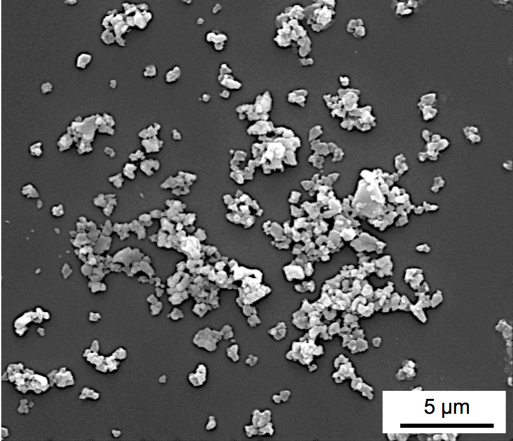
\includegraphics[width=\textwidth]{Chapter-2/Figures/Figure1.png}
	\caption{SEM image of as-received chemically purified Bayer Al$_{2}$O$_{3}$ powder used in this study.}
	\label{Ch2-figure:Figure1}
\end{figure}
%%%

\newpage
%%%
\begin{figure}[H]
	\centering
	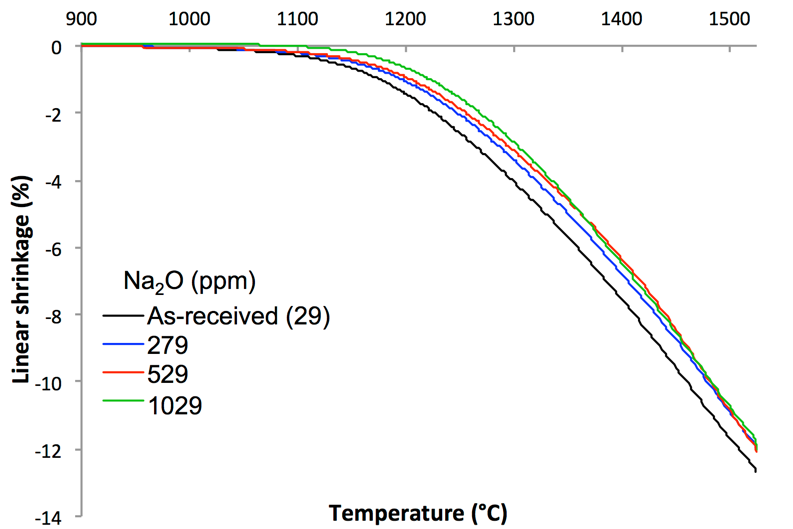
\includegraphics[width=\textwidth]{Chapter-2/Figures/Figure2.png}
	\caption{Dilatometer curves of as-received and singly Na$_{2}$O-doped samples heated at 10$^{\circ}$C/min to 1525$^{\circ}$C.}
	\label{Ch2-figure:Figure2}
\end{figure}
%%%

\newpage
%%%
\begin{figure}[H]
	\centering
	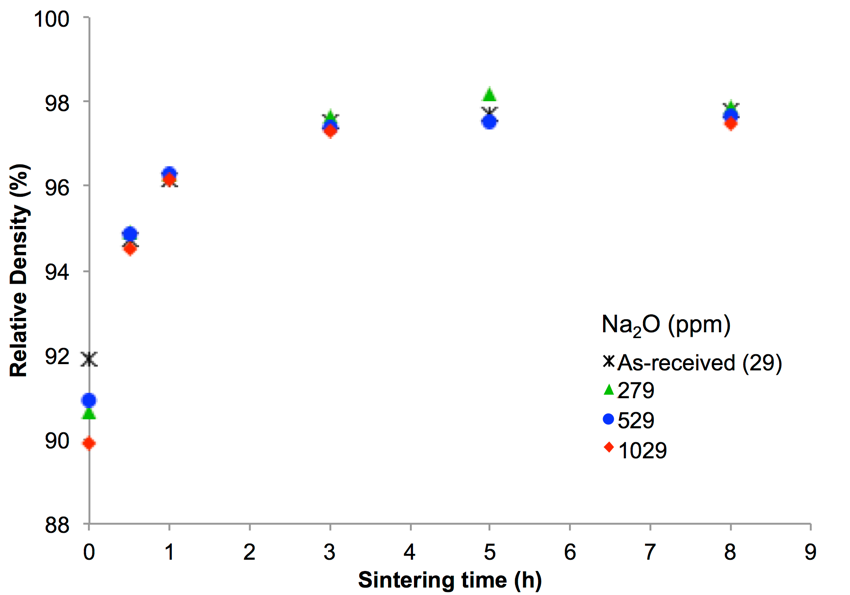
\includegraphics[width=\textwidth]{Chapter-2/Figures/Figure3.png}
	\caption{Densification kinetics of Bayer Al$_{2}$O$_{3}$ doped with different Na$_{2}$O concentrations and sintered at 1525$^{\circ}$C.}
	\label{Ch2-figure:Figure3}
\end{figure}
%%%

\newpage
%%%
\begin{figure}[H]
	\centering
	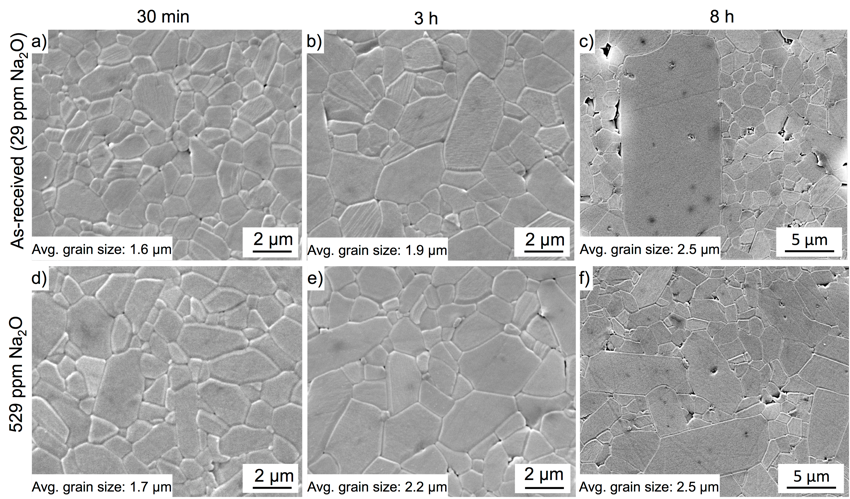
\includegraphics[width=\textwidth]{Chapter-2/Figures/Figure4.png}
	\caption{Microstructures of as-received and singly 529 ppm Na$_{2}$O doped samples after 30 min, 3 h and 8 h at 1525$^{\circ}$C.}
	\label{Ch2-figure:Figure4}
\end{figure}
%%%

\newpage
%%%
\begin{figure}[H]
	\centering
	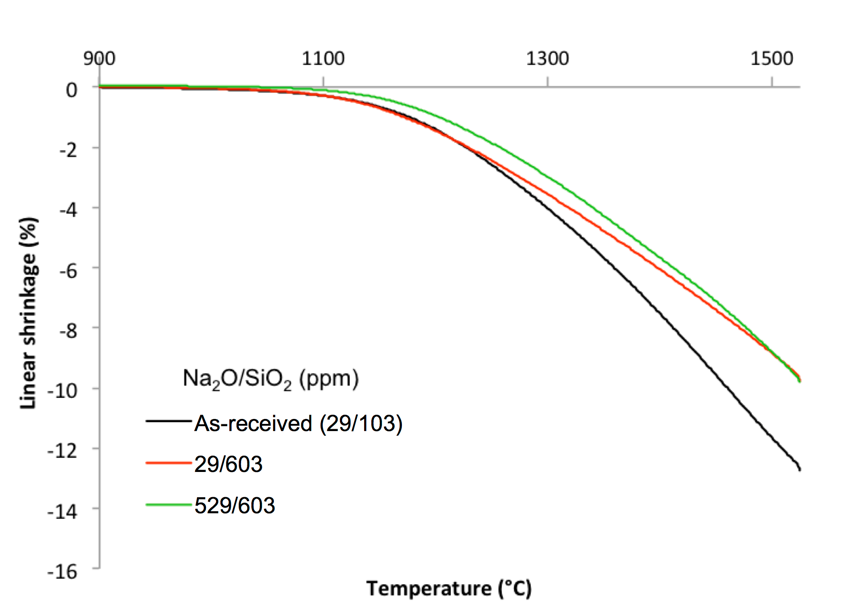
\includegraphics[width=\textwidth]{Chapter-2/Figures/Figure5.png}
	\caption{Dilatometer curves of as-received, singly SiO$_{2}$-doped, and Na$_{2}$O/SiO$_{2}$-doped Bayer Al$_{2}$O$_{3}$ heated at 10$^{\circ}$C/min to 1525$^{\circ}$C.}
	\label{Ch2-figure:Figure5}
\end{figure}
%%%

\newpage
%%%
\begin{figure}[H]
	\centering
	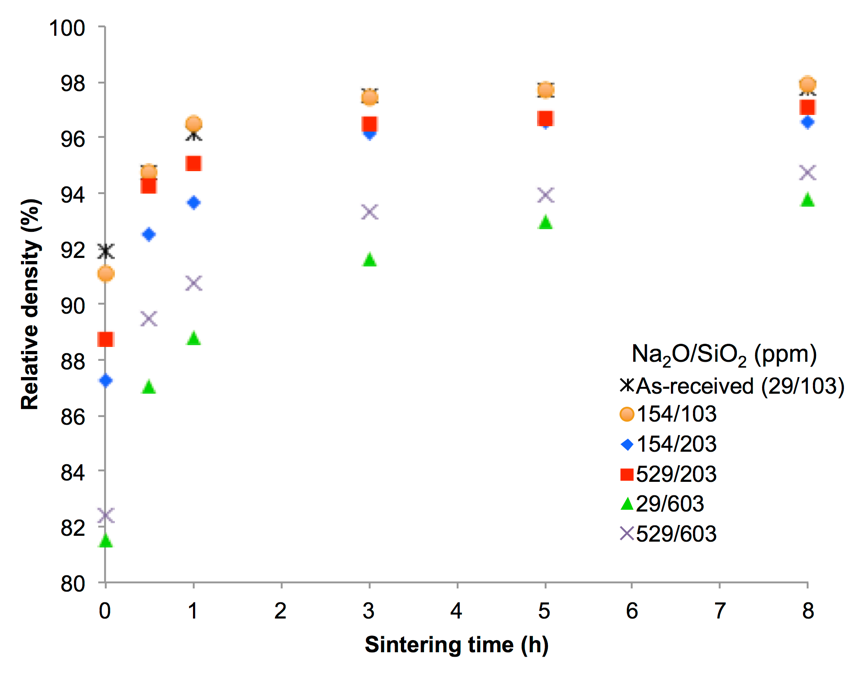
\includegraphics[width=\textwidth]{Chapter-2/Figures/Figure6.png}
	\caption{Densification kinetics of Bayer Al$_{2}$O$_{3}$ doped with different concentrations of Na$_{2}$O and SiO$_{2}$ at 1525$^{\circ}$C.}
	\label{Ch2-figure:Figure6}
\end{figure}
%%%

\newpage
%%%
\begin{figure}[H]
	\centering
	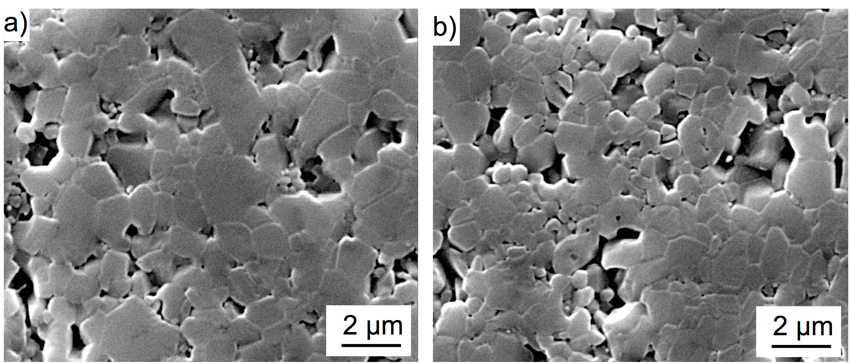
\includegraphics[width=\textwidth]{Chapter-2/Figures/Figure7.png}
	\caption{Microstructures of Bayer Al$_{2}$O$_{3}$ doped with a) 603 ppm SiO$_{2}$ and b) 529 ppm Na$_{2}$O and 603 ppm SiO$_{2}$ after heating at 1525$^{\circ}$C for 8h.}
	\label{Ch2-figure:Figure7}
\end{figure}
%%%

\newpage
%%%
\begin{figure}[H]
	\centering
	\includegraphics[width=\textwidth]{Chapter-2/Figures/Figure8.png}
	\caption{Micrographs of a sample doped with 1029 ppm Na$_{2}$O after sintering at 1525$^{\circ}$C for 3 h. The micrographs were recorded using a) a secondary electron detector and b) a backscattered electron detector. The arrows point at the platelet shaped beta alumina grains that form in samples doped with Na$_{2}$O. The samples were not thermally etched.}
	\label{Ch2-figure:Figure8}
\end{figure}
%%%

\newpage
%%%
\begin{figure}[H]
	\centering
	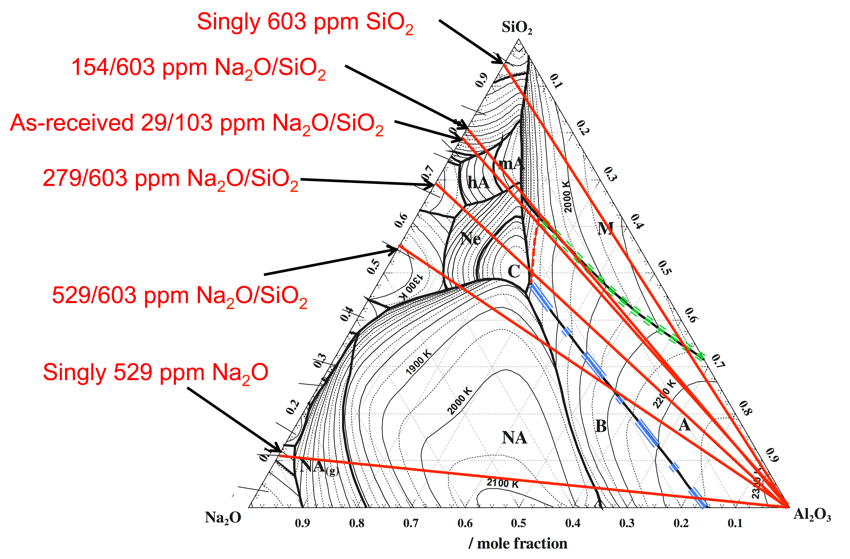
\includegraphics[width=\textwidth]{Chapter-2/Figures/Figure9.png}
	\caption{Liquidus projection of the Al$_{2}$O$_{3}$-SiO$_{2}$-Na$_{2}$O ternary phase diagram. The red solid lines are isoplethal cuts representing the samples investigated in this study. The red dashed line is the 1525$^{\circ}$C isotherm where $\alpha$-Al$_{2}$O$_{3}$ and liquid are in equilibrium. The blue dash-dot line and green dotted line are eutectic lines at which $\alpha$-Al$_{2}$O$_{3}$ and liquid is in equilibrium with $\beta$-Al$_{2}$O$_{3}$ or mullite, respectively.}
	\label{Ch2-figure:Figure9}
\end{figure}
%%%

\chapter{Powder Chemistry Effects on the Sintering Behavior of MgO-doped Bayer Alumina}

\section{Introduction}
Specialty aluminas are generally defined as a calcined or sintered alumina made from a Bayer processed feedstock. These aluminas have specific characteristics to improve their performance in commercial applications, such as defined primary crystal size, surface area, density and shrinkage, and chemical purities in the range of 99.0 - 99.8\%. The remaining 1.0 - 0.2\% consists of the intentionally added MgO dopant, and impurities such as Na$_{2}$O, CaO, Fe$_{2}$O$_{3}$, and SiO$_{2}$ that originate from the bauxite ore or the Bayer process itself. It is well known that trace (ppm) amounts of dopants or impurities can have a significant influence on the sintering of alumina \cite{Bae1994,Bae1997,Bae1993}. Since Coble's discovery of MgO doping to produce high-density translucent alumina, there has been high academic and commercial interest in understanding how small concentrations of dopants and impurities characteristic of specialty alumina affect sintering \cite{Bennison1990,Jorgensen1965,Heuer1979,Louet2005a,Park2000a}.

In chapter 2, the influence of Na$_{2}$O and SiO$_{2}$ on the sintering of MgO-free specialty alumina was investigated \cite{Frueh2016}. Na$_{2}$O was shown to initially retard the densification of MgO-free specialty alumina samples, but no effect was observed after extended sintering time (> 30 min) at 1525$^{\circ}$C, whereas the addition of SiO$_{2}$ to MgO-free specialty alumina formed a liquid phase and significantly retarded densification throughout the entire sintering process. Na$_{2}$O addition to SiO$_{2}$-doped samples increased the densification rate and degree of densification compared to singly SiO$_{2}$-doped samples. Based on phase equilibria, the solubility of Al$_{2}$O$_{3}$ in the liquid phase was shown to increase as the Na$_{2}$O concentration in the liquid grain boundary phase increases. Furthermore, a higher Na$_{2}$O concentration decreases the viscosity of the liquid phase, which further increases the densification rate. Hence, samples with high Na$_{2}$O/SiO$_{2}$ ratios ($\geq$0.5) showed higher densities than samples with lower Na$_{2}$O/SiO$_{2}$ ratios. 

MgO is commonly added to commercial alumina powders because it is known to improve sintering. Several reasonable mechanistic explanations for the beneficial effect of MgO include solute-drag, particle-pinning, modification of defect chemistry, increase of surface diffusivity, modification of a liquid phase, and modification of interfacial properties \cite{Bae1994}. A model that takes into account the redistribution of MgO and SiO$_{2}$ during the sintering of high purity alumina was reported by Handwerker et al. \cite{Handwerker1989} They proposed that MgO changes the segregation behavior of glass forming impurities such as SiO$_{2}$ by increasing their solubility in Al$_{2}$O$_{3}$. This mechanism was supported by the work of Gavrilov et al. \cite{Gavrilov1999} who demonstrated by high resolution secondary ion mass spectrometry that the dopants segregate strongly to grain boundaries when high purity Al$_{2}$O$_{3}$ is singly doped with either SiO$_{2}$ or MgO, but show a higher solubility in Al$_{2}$O$_{3}$ when co-doped with MgO and SiO$_{2}$ due to a defect mechanism in which Mg$^{2+}$ and Si$^{4+}$ occupy Al$^{3+}$ sites and compensate for each other's charge and strain. This model is of particular interest since it considers the direct interaction of MgO and SiO$_{2}$; an impurity known to negatively affect alumina densification. 

In this chapter we report how Na$_{2}$O and SiO$_{2}$ influence the sintering of 99.8 - 99.9\% pure specialty alumina doped with 380 ppm MgO. Dilatometry and sintering kinetics of MgO-free specialty alumina samples with similar Na$_{2}$O and SiO$_{2}$ concentrations from chapter 2 are compared to the present results to identify the stages at which MgO affects densification, and to identify key mechanisms that are responsible for the beneficial effect of MgO on the sintering of specialty alumina \cite{Frueh2016}. High-resolution transmission electron microscopy (TEM) and energy dispersive spectroscopy (EDS) measurements show the distribution of dopants/impurities on grain boundaries. First-principles calculations based on the density functional theory (DFT) were carried out to estimate the relative thermodynamic stability of MgO, SiO$_{2}$, and MgO+SiO$_{2}$ in the alumina lattice.


\section{Experimental}

A chemically purified MgO-doped specialty alumina powder (Almatis, Inc., Leetsdale, PA, USA) was chosen for this study. Earlier we studied the influence of SiO$_{2}$ and Na$_{2}$O on the sintering of MgO-free specialty alumina using a powder with similar physical and chemical characteristics as the powder used in this study \cite{Frueh2016}. Since the sample preparation procedures of the two powders were identical, the differences in sintering behavior after doping with similar Na$_{2}$O and SiO$_{2}$ concentrations should be attributable primarily to the difference in MgO concentration and its cross effects with Na$_{2}$O and SiO$_{2}$ \cite{Frueh2016}. 

Physical and chemical characteristics of the powder are shown in Table \ref{Ch3-table:table1} and Figure \ref{Ch3-figure:Figure1}. The powder was doped with up to 1000 ppm Na$_{2}$O and 500 ppm SiO$_{2}$ using sodium acetate (NaC$_{2}$H$_{3}$O$_{2.3}$H$_{2}$O, ACS grade, BDH, VWR International LLC, West Chester, PA, USA) and tetraethyl orthosilicate (Si(OC$_{2}$H$_{5}$)4), 98\%, Aldrich Chemical Company, Inc. Milwaukee, WI, USA), respectively, to obtain chemistries similar to commercial high purity specialty aluminas with different liquid volume fractions and different Na$_{2}$O/SiO$_{2}$ ratios, as shown in Table \ref{Ch3-table:table2}. The detailed doping procedures are described in chapter 2. 

Samples with green densities of 59.0 $\pm$ 0.5\% were fabricated for sintering studies by uniaxial and cold isostatic dry pressing (CIP, Autoclave engineers, Erie, Pa, USA) at 170 MPa and 200 MPa, respectively. The dry pressed cylinders were heated at 10 $^{\circ}$C/min to 1525 $^{\circ}$C in a thermomechanical analyzer (TMA, Linseis PT1600, Robbinsville, NJ, USA) to record the shrinkage during heating. The kinetics of sintering of samples at 1450 $^{\circ}$C and 1525 $^{\circ}$C were investigated for up to 8 h. The samples were heated at 10 $^{\circ}$C/min to 1200 $^{\circ}$C and then at 5 $^{\circ}$C/min to the final sintering temperature. The average grain size and density were measured by the linear intercept (ASTM Standard E112-96) \cite{Standard2013} and Archimedes methods (ASTM standard B962-15), \cite{Standard2015} respectively. The structure and chemistry of grain boundaries were investigated by transmission electron microscopy (TEM) and energy dispersive x-ray spectroscopy EDS using a dual aberration corrected FEI Titan \cite{Bae1993} field emission microscope operated at 300 kV and FEI Talos (FEI, Hillsboro, OR, USA) field emission microscope at 200 kV. The EDS on both microscopes is an FEI Super-X system consisting of four SDDs (Silicon Drift Detectors) with a solid angle of 0.9 srad.  The samples for TEM and EDS were air-quenched from the sintering temperature and prepared using a focused ion beam (Quanta 200 3D Dual Beam FIB, FEI, Hillsboro, OR, USA). Grain boundaries were chosen for analysis that were oriented parallel to the TEM beam in order to accurately measure grain boundary widths in the 2D projection images and EDS profiles. Chemical analyses were performed by inductively coupled plasma (ICP) emission spectroscopy (iCap 6000, Thermo Fischer Scientific, Inc., Waltham, MA, USA) after alumina samples were acid digested in a microwave digestion unit equipped with a Teflon sample holder (MARS M, CEM Corp., Matthews, NC, USA).

\section{Computational Methodology}

DFT-based first-principles calculations were carried out at 0 K to investigate the thermodynamic stability of clustered defects in the $\alpha$-alumina structure. The energy at 0 K without the contribution of the zero-point vibrational energy $E_{0}$ was obtained by an equation of state (EOS) fitting using the four-parameter Birch-Murnaghan (BM4) equation as follows \cite{Shang2010}:

%%
\begin{equation}
\label{Ch3-eq: EOS}
E_{0}(V) = a + bV^{- \frac{2}{3}} + cV^{- \frac{4}{3}} + dV^{-2}
\end{equation}
%%

\noindent where $a$, $b$, $c$, and $d$ are fitting parameters. The EOS fitting is achieved through an energy-volume (E-V) curve of at least 5 different volumes based on the methodology discussed by Shang et al. \cite{Shang2010}. The Helmholtz energy $F(V,T)$ can be predicted as a function of temperature $T$ and volume $V$ via \cite{Shang2010,Wang2004}:

%%
\begin{equation}
\label{Ch3-eq: helmholtz}
F(V,T) = E_{0}(V) + F_{vib}(V,T) + F_{T-el}(V,T)
\end{equation}
%%

\noindent where $F_{vib}$ is the temperature-dependent vibrational contribution, and $F_{T-el}$ is the thermal electronic contribution. At ambient pressure, the Helmholtz energy of the system is equal to the Gibbs energy. 

The vibrational contribution was obtained using the Debye-Gr\"uneisen model \cite{Shang2010}:

%%
\begin{equation}
\label{Ch3-eq: Fvib}
F_{vib}(V,T) = \frac{9}{8} k_{B} \theta_{D}(V) - k_{B}T \left [D\left( \frac{\theta_{D} (V)}{T} \right) + 3 ln \left(1-e^{-\theta_{D}(V)/T} \right) \right]
\end{equation}
%%

\noindent where $\theta_{D}$ is the Debye temperature, $T$ the temperature, and D[$\theta_{D}$(V)/T] the Debye function. The Debye temperature can be calculated by: 

%%
\begin{equation}
\label{Ch3-eq: debyetT}
\theta_{D} = s \frac{(6\pi^{2})^{\frac{1}{3} \hbar}}{k_{B}} V_{0}^{\frac{1}{6}} \left(\frac{B_{0}}{M} \right)^{\frac{1}{2}} \left(\frac{V_{0}}{V} \right)^{\gamma}
\end{equation}
%%

\noindent where $s$ is the Debye temperature scaling factor, $\gamma$ the Gr\"uneisen parameter determined by the pressure derivative of bulk modulus $B'$, $B_{0}$ the equilibrium bulk modulus, $M$ the atomic mass, and $V_{0}$ the equilibrium volume. Here, the equilibrium properties $V_{0}$, $B_{0}$, and $B'$ are estimated from the EOS of Eq. \ref{Ch3-eq: EOS}. The methodology by Liu et al. \cite{Liu2015} was used to calculate the scaling factor of Al$_{2}$O$_{3}$: 

%%
\begin{equation}
\label{Ch3-eq: scalingfactor}
s(\nu) = 3^{\frac{5}{6}} \left( 4 \sqrt{2} \left(\frac{1+\nu}{1-\nu}\right)^{\frac{3}{2}} + \left(\frac{1+\nu}{1-\nu}\right)^{\frac{3}{2}}\right)^{-\frac{1}{3}}
\end{equation}
%%

\noindent where $\nu$ is the Poisson's ratio, which was calculated by Shang et al. \cite{Shang2007c}. The thermal electronic contribution was estimated based on the electronic density of states and the Fermi-Dirac statistics \cite{Wang2004}.

In the present work, the Vienna Ab-initio Simulation Package (VASP) was used to perform the first-principles calculations \cite{Kresse1996}. The projector augmented-wave (PAW) \cite{Kresse1999,Blochl1994} method was utilized to describe the electron-ion interactions with the exchange correlation functional given by the generalized gradient approximation (GGA-PW91) \cite{Perdew1992}. A sigma value of 0.2 eV and a plane wave energy cutoff of 1.3 times higher than the highest default cutoff were adopted. The Brillouin zone sampling was carried out with Bl\"ochl corrections using a gamma centered Monkhorst-Pack (MP) scheme \cite{Blochl1994,Monkhorst1976a}. The automated k-points grid generator in VASP was employed with a subdivision length of 80. The energy convergence criterion of the electronic self-consistency was set at 10$^{-5}$ eV/atom for all calculations.

The energies of charge, site, and mass balanced defects in $\alpha$-alumina were calculated for defect clusters, i.e. the defects are located next to each other, since this has been shown to be the most stable configuration \cite{Atkinson2003}. The geometric arrangements of each of the clusters were chosen based on previous computational work. Multiple authors showed that a 30-40 atom supercell of Al$_{2}$O$_{3}$ is sufficient to calculate non-charged defects \cite{Atkinson2003,Grimes1994,Lagerlof1998,Xiang2015,Sarsam2013}. Multiple authors have studied charged and clustered defects in Al$_{2}$O$_{3}$ \cite{Atkinson2003,Grimes1994,Lagerlof1998,Xiang2015,Sarsam2013}. They showed that different geometric arrangements and supercell size result in little difference in energy and that the impurity atoms prefer to be clustered due to the binding energy \cite{Atkinson2003,Grimes1994,Lagerlof1998,Xiang2015,Sarsam2013}. Using this methodology, supercells were generated in the present work with Mg and/or Si clustered, i.e. the Mg-cluster having two Mg atoms substituted for two Al atoms and an oxygen vacancy as nearest neighbors, the Si-cluster having three Si atoms substituted for three Al atoms and an Al vacancy, and the Mg+Si-cluster having one Mg and one Si substituted for two Al atoms. 

\section{Sintering and Microstructure Analysis}

In chapter 2, it was shown that a glass phase can form during sintering of specialty alumina. Table \ref{Ch3-table:table2} shows the amounts of liquid in the samples at 1525 $^{\circ}$C estimated from the Al$_{2}$O$_{3}$-Na$_{2}$O-SiO$_{2}$ and Al$_{2}$O$_{3}$-MgO-SiO$_{2}$ phase diagrams based on the amount of SiO$_{2}$, Na$_{2}$O and MgO \cite{Mao2005}. It can be seen that the glass volume fraction increases from 0.03 vol.\% for SiO$_{2}$ concentrations of 82 ppm to 0.21 vol.\% for SiO$_{2}$ concentrations of 582 ppm at 1525 $^{\circ}$C. 

Figure \ref{Ch3-figure:Figure2} shows the dilatometry curves of MgO-doped and MgO-free \cite{Frueh2016} samples with different Na$_{2}$O and SiO$_{2}$ concentrations heated at 10 $^{\circ}$C/min to 1525$^{\circ}$C. For samples with SiO$_{2}$ concentrations of 582 ppm the estimated amount of liquid increases from 0.18 vol.\% to 0.21 vol.\% during heating from 1250 $^{\circ}$C to 1525 $^{\circ}$C, and for samples with 82 ppm SiO$_{2}$ the amount of liquid phase is estimated from the phase diagram to increase from 0.026 vol.\% to 0.030 vol.\% during heating from 1250 $^{\circ}$C to 1525 $^{\circ}$C. 

Figure \ref{Ch3-figure:Figure2}a shows that the onset of densification of MgO-doped specialty alumina is shifted to higher temperatures for samples with higher Na$_{2}$O concentrations. Samples with 560 ppm Na$_{2}$O shrink 1\% less than samples with 60 ppm Na$_{2}$O after heating to 1525 $^{\circ}$C. In both the MgO-doped and the MgO-free powders, higher SiO$_{2}$ concentrations retard densification at $\sim$1250 $^{\circ}$C. However, the retardation caused by higher SiO$_{2}$ concentrations is less severe in the MgO-doped powder than in the MgO-free powder; e.g. already at 1300 $^{\circ}$C, MgO-doped powder samples with 582 ppm SiO$_{2}$ (after the addition of 500 ppm SiO$_{2}$) shrink 0.2\% less and are 0.5\% less dense than samples with 82 ppm SiO$_{2}$, whereas samples of the MgO-free powder with 603 ppm SiO$_{2}$ shrink 0.5\% less and are 3.2\% less dense than samples with 103 ppm SiO$_{2}$. After reaching 1525 $^{\circ}$C the dilatometry curves show that MgO-doped samples with 582 ppm SiO$_{2}$ (0.21 vol.\% glass) shrink 1.8\% less and are 5.4\% less dense than MgO-doped samples with 82 ppm SiO$_{2}$ (0.03 vol.\% glass). In contrast, the retardation of densification caused by the addition of 500 ppm SiO$_{2}$ to the MgO-free powder results in 3.0\% less linear shrinkage and 8.7\% lower relative densities after heating to 1525 $^{\circ}$C. MgO-doped (380 ppm) powder samples with 560 ppm Na$_{2}$O and 582 ppm SiO$_{2}$ shrink $\sim$2.5\% less than samples with 60 ppm Na$_{2}$O and 82 ppm SiO$_{2}$ after reaching 1525 $^{\circ}$C, and MgO-free powder samples with 529 ppm Na$_{2}$O and 603 ppm SiO$_{2}$ shrink $\sim$3.0\% less than samples with 29 ppm Na$_{2}$O and 103 ppm SiO$_{2}$ after reaching 1525 $^{\circ}$C.

Figure \ref{Ch3-figure:Figure3}a and b show how the sintering kinetics of MgO-doped and MgO-free \cite{Frueh2016} alumina are affected by Na$_{2}$O and SiO$_{2}$ after heating at 1450 $^{\circ}$C and 1525 $^{\circ}$C for up to 8 h. The density of samples with higher SiO$_{2}$ concentrations, i.e. higher glass concentrations, is lower for all hold times at 1450 $^{\circ}$C and 1525 $^{\circ}$C. At 1450 $^{\circ}$C MgO-doped powder samples with 0.19 vol.\% glass phase (582 ppm SiO$_{2}$) are 6-7\% less dense than samples with 0.027 vol.\% glass phase (82 ppm SiO$_{2}$), for all hold times (Figure \ref{Ch3-figure:Figure3}a). At 1525 $^{\circ}$C MgO-doped powder samples with 0.21 vol.\% glass phase are $\sim$11\% and $\sim$2\% less dense than samples with 0.03 vol.\% glass phase after heating for 0 h and 8 h, respectively, and samples with 0.03 vol.\% glass phase reach densities >98\% after 1 h, whereas samples with 0.066 and 0.21 vol.\% glass phase are only $\sim$96\% and $\sim$94\% dense, respectively (Figure \ref{Ch3-figure:Figure3}b). 

The effect of Na$_{2}$O concentration on densification strongly depends on glass phase concentration. In all samples a higher Na$_{2}$O concentration initially retards densification. For example, after 0 h at 1450 $^{\circ}$C the relative density of samples with 0.03 vol.\% glass phase and 560 ppm Na$_{2}$O is $\sim$3\% lower than the relative density of samples containing the same amount of glass phase and 60 ppm Na$_{2}$O.  However, there is no difference in sintered density after 3 h at either 1450 $^{\circ}$C or 1525 $^{\circ}$C. For samples with higher glass phase concentrations (e.g., 0.21 vol.\%) the effect of Na$_{2}$O on the densification is not straightforward, due to the changing Na$_{2}$O/SiO$_{2}$ ratio from 0.1 to 0.9 (Table \ref{Ch3-table:table2}). Samples with 0.21 vol.\% glass phase and Na$_{2}$O/SiO$_{2}$ ratios of 0.9 are 1-2\% denser than samples with 0.21 vol.\% glass phase and Na$_{2}$O/SiO$_{2}$ ratios of 0.1. However, after 30 min at 1525 $^{\circ}$C the relative density of samples with 0.21 vol.\% glass phase and Na$_{2}$O/SiO$_{2}$ ratios of 0.9 in the glass phase is 0.9\% lower than the relative density of samples with 0.21 vol.\% glass phase and Na$_{2}$O/SiO$_{2}$ ratios of 0.1 in the glass phase, and after 1 h or longer at 1525 $^{\circ}$C there is no difference in relative density. Samples with 0.066 vol.\% glass phase are 98.3 - 98.6\% dense after 8 h at 1525 $^{\circ}$C, and samples with 0.21 vol.\% glass phase are 97.1\% - 97.5\% dense after 8 h at 1525 $^{\circ}$C. 

Comparing the as-received MgO-free and MgO-doped powders with 0.03 vol.\% glass phase shows that doping with 380 ppm MgO leads to 1\% higher densities for all hold times at 1525 $^{\circ}$C (Figure \ref{Ch3-figure:Figure3}b and c) \cite{Frueh2016}. After 8 h at 1525 $^{\circ}$C the MgO-doped samples with 0.21 vol.\% glass phase are $\sim$2\% less dense than samples with 0.03 vol.\% glass phase, whereas the addition of 500 ppm SiO$_{2}$ (total of 603 ppm SiO$_{2}$ and 0.22 vol.\% glass) to the MgO-free powder leads to $\sim$4\% less dense samples \cite{Frueh2016}. MgO-free and MgO-doped specialty alumina samples containing 0.22 and 0.21 vol.\% glass phase, respectively, and global Na$_{2}$O/SiO$_{2}$ ratios of 0.9 show initial retardation of densification compared to samples with Na$_{2}$O/SiO$_{2}$ ratios of 0.1, but have higher densities than samples with Na$_{2}$O/SiO$_{2}$ ratios of 0.1 after further heating. This increased densification can be explained by the increased solubility of Al$_{2}$O$_{3}$ into the liquid grain boundary phase and the higher diffusivity (lower viscosity of the grain boundary phase) as the Na$_{2}$O/SiO$_{2}$ ratio increases \cite{Frueh2016,Kwon1991}. However, after hold times of 1 h or longer at 1525 $^{\circ}$C, MgO-free powder samples with 0.22 vol.\% glass phase and Na$_{2}$O/SiO$_{2}$ ratios of 0.9 are 1\% denser than samples with 0.22 vol.\% glass phase and Na$_{2}$O/SiO$_{2}$ ratios of 0.1, whereas MgO-doped powder samples with 0.21 vol.\% and Na$_{2}$O/SiO$_{2}$ ratios of 0.9 have the same densities as samples with 0.21 vol.\% glass phase and Na$_{2}$O/SiO$_{2}$ ratios of 0.1. 

The microstructures of samples with different vol.\% glass phase and different Na$_{2}$O/SiO$_{2}$ ratios heated at 1525 $^{\circ}$C for 8 h are shown in Figure \ref{Ch3-figure:Figure4}. Samples with 60 ppm Na$_{2}$O show mostly equiaxed grains, regardless of the glass phase concentration in the samples (Figures \ref{Ch3-figure:Figure4}a and c). Samples with 560 ppm Na$_{2}$O (Figures  \ref{Ch3-figure:Figure4}b and d) show more facetted $\alpha$-Al$_{2}$O$_{3}$ grains and appear to have a wider grain size distribution than samples with 60 ppm Na$_{2}$O. These effects are more pronounced in samples with higher glass concentrations. The grain sizes of samples with 0.21 vol.\% glass are less than the grain sizes of samples with 0.03 vol.\% glass phase. 

The average grain sizes of samples with different vol.\% glass phase and different Na$_{2}$O/SiO$_{2}$ ratios are plotted as a function of relative density in Figure \ref{Ch3-figure:Figure5}. Grain growth starts when the final sintering stage is reached, between 85 and 92\% relative density. Samples with 0.03 vol.\% glass phase and 60 ppm Na$_{2}$O show a three-fold increase in grain size, from 0.5 $\mu$m to $\sim$1.5 $\mu$m, when the relative density increases from 68\% to 99\%, and samples with 0.03 vol.\% glass phase and 560 ppm Na$_{2}$O have a somewhat larger grain size of 2.2 $\mu$m at 99\% relative density. When relative densities of $\sim$99\% are reached in samples with 0.03 vol.\% glass, the grain size increases to 3.1 - 3.4 $\mu$m when heated at 1525 $^{\circ}$C for 8 h. Samples with higher glass concentrations have a similar trajectory up to 92\% density. However, at densities >92 \% grain growth is enhanced in samples with higher glass concentrations, and at 97 - 97.5\% density higher glass phase concentrations of 0.21 and 0.17 vol.\% lead to a larger grain size of 2.6 and 2.4 $\mu$m, respectively, compared to samples with 0.03 vol.\% glass phase ($\sim$1.5 $\mu$m grain size). 

\section{Mechanistic Interpretation}

If the mechanism of MgO increasing the solubility of SiO$_{2}$ in alumina, as proposed by Handwerker et al., \cite{Handwerker1989} is responsible for the improved sintering behavior of alumina, then the amount of liquid phase in MgO-doped alumina should be less than calculated and less than in MgO-free samples, and, the grain boundary thickness in MgO-doped alumina should be less than in MgO-free powder. The reduced grain boundary thickness in MgO-doped alumina should lead to an change in grain boundary chemistry and different sintering behavior after this co-dissolution has occurred compared to MgO-free alumina. 

Comparing the dilatometry curves and sintering kinetics of MgO-doped and MgO-free specialty alumina powders with different chemistries indicates that there are two stages at which MgO affects densification. At 1250 $^{\circ}$C increased glass phase content retards densification, and at the same stage there is an enhancement of densification due to MgO. This suggests that there is a direct interaction between the glass phase and MgO at this stage, where MgO mitigates the negative effect of the glass phase, probably by modifying the properties of the liquid grain boundary phase. The Al$_{2}$O$_{3}$-SiO$_{2}$-MgO phase diagram suggests that MgO increases the solubility of Al$_{2}$O$_{3}$ in the liquid, and MgO can lower the viscosity of the glass melt, \cite{Wu2015} which results in higher diffusion coefficients. The enhanced diffusion associated with the lower viscosity and higher solubility of Al$_{2}$O$_{3}$ in the glass phase can explain why MgO positively affects the sintering of alumina at stages when SiO$_{2}$ would negatively affect densification. 

The second stage at which MgO affects densification is after 1 h at 1525 $^{\circ}$C. MgO-free powder samples with 0.22 vol.\% glass phase and Na$_{2}$O/SiO$_{2}$ ratios of 0.9 have 1-2\% higher relative densities than samples with 0.22 vol.\% glass phase and Na$_{2}$O/SiO$_{2}$ ratios of 0.1 for all hold times at 1525 $^{\circ}$C. In previous work we calculated an expected grain boundary thickness of 1.3 nm for samples with 0.22 vol.\% glass phase after 3 h at 1525 $^{\circ}$C, based on the observed grain size of 1.6 $\mu$m. The addition of 500 ppm Na$_{2}$O increases the Na$_{2}$O/SiO$_{2}$ ratio from 0.1 to 0.9, which modifies the liquid grain boundary phase and enhances densification \cite{Frueh2016}. Figure \ref{Ch3-figure:Figure6} shows a high-resolution TEM image of a grain boundary of a MgO-free powder \cite{Frueh2016} sample (2 ppm MgO) with 0.22 vol.\% glass phase and a Na$_{2}$O/SiO$_{2}$ ratio of 0.9 after 3 h at 1525 $^{\circ}$C. It can be seen that the measured grain boundary thickness of 1.7 nm is close to the grain boundary thickness calculated based on the amount of glass phase in the sample. MgO-doped powder samples with 0.21 vol.\% glass phase and Na$_{2}$O/SiO$_{2}$ ratios of 0.9 have 1-2\% higher densities than samples with 0.21 vol.\% glass phase and Na$_{2}$O/SiO$_{2}$ ratios of 0.1 for most hold times at 1450 $^{\circ}$C and for hold times < 30 min at 1525 $^{\circ}$C. This difference in densification behavior is similar to the densification behavior of MgO-free powder samples, which suggests the presence of a liquid phase that is modified by Na$_{2}$O, as seen in the MgO-free alumina samples. 

Figure \ref{Ch3-figure:Figure7}a shows a high resolution TEM image of a grain boundary in an MgO-doped alumina sample with 0.21 vol.\% glass phase and a Na$_{2}$O/SiO$_{2}$ ratio of 0.9 after 0 h at 1525 $^{\circ}$C. The measured grain boundary thickness of $\sim$1.4 nm for this sample is in agreement with the theoretically estimated \cite{Frueh2016} grain boundary thickness. However, after 1 h or longer at 1525 $^{\circ}$C, samples with 0.21 vol.\% glass and Na$_{2}$O/SiO$_{2}$ ratios of 0.9 have the same densities as samples with 0.21 vol.\% glass and Na$_{2}$O/SiO$_{2}$ ratios of 0.1, and the grain boundary thicknesses of those samples after 3 h at 1525 $^{\circ}$C are $\sim$0.3 nm (Figure \ref{Ch2-figure:Figure7}b) and substantially thinner than the calculated grain boundary thicknesses of 1.4 nm.

The thinner grain boundary suggests that the addition of MgO causes a reduction of the amount of liquid phase in the grain boundaries after longer time at 1525 $^{\circ}$C. In the literature it is reported that excess liquid phase, after an equilibrium grain boundary thickness \cite{Subramaniam2006} is reached, can accumulate in triple pockets. However, we did not observe any triple pockets in the 380 ppm MgO-doped samples with 0.21 vol.\% glass. Therefore, the impurities and dopants that formed the liquid phase after 0 h have to be distributed elsewhere in the sample after 3 h at 1525 $^{\circ}$C. Since SiO$_{2}$-containing second phases, such as mullite or cordierite, were not observed in the samples, we hypothesize that SiO$_{2}$ and MgO form a solid solution in $\alpha$-alumina, as proposed by Handwerker et al. \cite{Handwerker1989}. This co-dissolution mechanism would significantly reduce the total amount of SiO$_{2}$ and, therefore, the liquid phase content in the samples and in the grain boundaries. 

The EDS maps in Figure \ref{Ch2-figure:Figure8} show the distribution of Si around a grain boundary in MgO-doped samples with a calculated glass concentration of 0.21 vol.\% after 0 h and 3 h at 1525 $^{\circ}$C. Figure \ref{Ch2-figure:Figure9} shows the corresponding EDS line scans for Si and Mg across the grain boundaries. It can be seen that after 0 h at 1525 $^{\circ}$C SiO$_{2}$ and MgO are strongly concentrated in the grain boundaries, and a chemical grain boundary thickness, $\delta_{chem}$, of $\sim$1.7 nm is estimated (Figures \ref{Ch2-figure:Figure8}a and \ref{Ch2-figure:Figure9}a), which is close to the structural grain boundary thickness of 1.4 nm measured from the high resolution TEM image (Figure \ref{Ch2-figure:Figure7}a). After 3 h at 1525 $^{\circ}$C MgO and SiO$_{2}$ are still concentrated on the grain boundary, however, the chemical grain boundary thickness, $\delta_{chem}$, is $\sim$3.2 nm (Figure \ref{Ch2-figure:Figure8}b and \ref{Ch2-figure:Figure9}b) and substantially thicker than the observed structural grain boundary thickness, $\delta_{str}$, of $\sim$0.3 nm (Figure \ref{Ch2-figure:Figure7}b). This difference in structural and chemical grain boundary thickness after 3 h supports the argument that MgO and SiO$_{2}$ form a solid solution in the alumina lattice in the near grain boundary region. If we assume that equal amounts of MgO and SiO$_{2}$ dissolve into the alumina lattice to form the proposed defect complex, and that all MgO in the sample is consumed by this process, then 380 ppm SiO$_{2}$ must be removed from the amorphous grain boundary phase. This would leave 202 ppm SiO$_{2}$ in the grain boundaries to form the amorphous film with a calculated grain boundary thickness of 0.5 nm, which is close to the observed grain boundary thickness of 0.3 nm \cite{Frueh2016}.

To further evaluate whether MgO and SiO$_{2}$ form a solid solution in $\alpha$-alumina we conducted first-principles calculations based on density functional theory to gain insight into the thermodynamic stability of Mg$^{2+}$ and Si$^{4+}$ by themselves and together in the $\alpha$-alumina structure. To ensure the accuracy of the calculations, the lattice parameters and energy of the $\alpha$-alumina structure without any substitutions are compared with previous experiments and calculations in Table \ref{Ch3-table:table3}. It can be seen that the calculated lattice parameters match well with experimental values and lattice parameters from previous first-principles calculations \cite{Jain2013,MaterialsProject,Graham1960_595,Bergerhoff1983,Karlsruhe,Atkinson2003}. The difference between the present and past first-principles calculations can be attributed to the different input parameters used. 

We calculated the energy of a unit cell of the α-alumina structure with substitutions according to the following balanced equations:\newline
\newline
\noindent Mg-Cluster: 
\begin{equation}
\label{Ch3-eq: Mgcluster}
2MgO + 2Al_{Al}^{x} + O_{O}^{x} \longrightarrow 2Mg_{Al}^{'} + V_{O}^{^{..}} + Al_{2}O_{3}
\end{equation}
%%
\newline
\noindent Si-Cluster:
\begin{equation}
\label{Ch3-eq: Sicluster}
3SiO_{2} + 4Al_{Al}^{x} \longrightarrow 3Si_{Al}^{^{.}} + V_{Al}^{'''} + 2Al_{2}O_{3}
\end{equation}
%%
\newline
\noindent Mg+Si-Cluster:
\begin{equation}
\label{Ch3-eq: MgSicluster}
MgO + SiO_{2} + 2Al_{Al}^{x} \longrightarrow Mg_{Al}^{'} + Si_{Al}^{^{.}} + Al_{2}O_{3}
\end{equation}
%%


\noindent Defect simulations of aliovalent cation substitutions in alumina \cite{Atkinson2003} showed that the dominant compensation mechanisms for Mg$^{2+}$ and Si$^{4+}$ by themselves in alumina are the formation of oxygen and aluminum vacancies, respectively (Eq.\ref{Ch3-eq: Mgcluster} and \ref{Ch3-eq: Sicluster}). In Eq. \ref{Ch3-eq: MgSicluster} Mg$^{2+}$ and Si$^{4+}$ compensate for each other's charge and the formation of vacancies or interstitials is unnecessary to account for dissolution in the alumina lattice. The calculations were carried out for clustered defects since they are lower in energy than isolated defects \cite{Atkinson2003}. The structures were relaxed and the formation energies as a function of temperature with bulk Al$_{2}$O$_{3}$ as the reference state are plotted in Figure \ref{Ch3-figure:Figure10}. It can be seen that the formation energy for the Mg+Si-cluster, $E_{Form}^{Mg+Si}$, is lower than the formation energies of the Mg-cluster, $E_{Form}^{Mg}$, and the Si-cluster, $E_{Form}^{Si}$, which indicates that the Mg+Si-cluster is more stable than the Mg-cluster and the Si-cluster. Since two Mg$^{2+}$ ions and three Si$^{4+}$ ions are necessary to form the Mg-cluster and Si-cluster, respectively, but only one Mg$^{2+}$ and one Si$^{4+}$ are required to form the Mg+Si-cluster, the formation energies of the clusters can be compared by 

%%
\begin{equation}
\label{Ch3-eq: eform}
\bigtriangleup E_{Form}=E_{Form}^{Mg+Si} - \left( \frac{1}{3} E_{Form}^{Si} + \frac{1}{2}E_{Form}^{Mg} \right)
\end{equation}
%%

\noindent The formation energy difference, $\bigtriangleup E_{Form}$, is plotted in Figure \ref{Ch3-figure:Figure10} and it can be seen that $\bigtriangleup E_{Form}$ is negative at all temperatures, which means that the Mg+Si-cluster is more energetically favored to form than the Mg-cluster or Si-cluster. This indicates that MgO and SiO$_{2}$ have a higher co-solubility in $\alpha$-alumina than MgO or SiO$_{2}$ by themselves. In $\alpha$-alumina the Al$^{3+}$ cation sites are 6-fold coordinated and Al$^{3+}$ has an effective ionic radius of 53.5 pm, while the radii of Mg$^{2+}$ and Si$^{4+}$ are 72 pm and 40 pm, respectively. Therefore, Mg$^{2+}$ and Si$^{4+}$ can compensate for each other's size and charge difference relative to Al$^{3+}$ in the $\alpha$-alumina lattice, which explains the lower energy of the Mg+Si-cluster. The stable phases for MgO and/or SiO$_{2}$ and Al$_{2}$O$_{3}$ are spinel, cordierite, and mullite. However, we hypothesize that if both MgO and SiO$_{2}$ are present at low concentrations, then it is more favorable for MgO and SiO$_{2}$ to form a solid solution in the $\alpha$-alumina structure than to form a second phase or remain in the grain boundaries as a siliceous liquid phase. 

The described mechanism could also influence the distribution of other oxides in the samples, such as Fe$_{2}$O$_{3}$, CaO, and Na$_{2}$O. Figure \ref{Ch3-figure:Figure11} shows the element distribution obtained from EDS of two grain boundaries in samples sintered at 1525 $^{\circ}$C for 0 h and 3 h, respectively. Figures \ref{Ch3-figure:Figure11}a and e show the segregation of MgO to the grain boundaries after 0 h and 3 h, respectively, and it can be seen that after 0 h at 1525 $^{\circ}$C Mg is more strongly concentrated in the grain boundary than after 3 h at 1525 $^{\circ}$C, due to the mechanism described above. From Figures \ref{Ch3-figure:Figure11}b and f it can be seen that there is no segregation of Fe$_{2}$O$_{3}$ and we believe that Fe$_{2}$O$_{3}$ is in solid solution in the alumina lattice, \cite{Atkinson2003} since the Al$_{2}$O$_{3}$-Fe$_{2}$O$_{3}$ phase diagram shows considerable solubility \cite{Raghavan2010}. Figures \ref{Ch3-figure:Figure11}c, d, g, and h show that there is a slightly higher Na and Ca signal coming from the grain boundaries, indicating that Na and Ca segregate to the grain boundaries and are components of the liquid grain boundary phase. Ca is more concentrated in the grain boundary after 3 h at 1525 $^{\circ}$C, due to the narrower grain boundary thickness (Figure \ref{Ch3-figure:Figure7}b). 

It can be seen that the Na signal after 0 h at 1525 $^{\circ}$C (Figure \ref{Ch3-figure:Figure11}c) shows a slight segregation of Na to the grain boundary, but after 3 h at 1525 $^{\circ}$C (Figure \ref{Ch3-figure:Figure11}g) no segregation can be observed. It should also be noted that it is challenging to detect Na using EDS since the Na signal disappears quickly after the high-voltage electron beam is focused on the grain boundary. Therefore, we believe that there is still Na on the grain boundaries, even though the EDS map does not show an increased Na signal. However, since the Na signal is lower, we believe that after 3 h at 1525 $^{\circ}$C there is less Na$_{2}$O on the grain boundaries than after 0 h at 1525 $^{\circ}$C. The reduced amount of Na might be a result of volatilization of Na$_{2}$O during sintering. Figure \ref{Ch3-figure:Figure12} shows the influence of sintering time and temperature on the Na$_{2}$O concentration, obtained by ICP analysis, during sintering for samples with target concentrations of 560 ppm Na$_{2}$O. It can be seen that there is no observable Na$_{2}$O loss as a function of temperature up to 1525 $^{\circ}$C (Figure \ref{Ch3-figure:Figure12}a), but after heating to 1600 $^{\circ}$C there is a loss of $\sim$200 ppm or a $\sim$35\% decrease in Na$_{2}$O concentration. After sintering at 1525 $^{\circ}$C for 30 min the Na$_{2}$O concentration decreases by about 200 ppm, but remains constant at $\sim$350 ppm when heated to 1525 $^{\circ}$C for up to 8 h (Figure \ref{Ch3-figure:Figure12}b). Between 1300 $^{\circ}$C and 1525 $^{\circ}$C the Na$_{2}$O concentration is constant at $\sim$510 ppm, which is 50 ppm below the target level. The lower Na$_{2}$O concentration might be due to volatilization at earlier stages. During heating at 1525 $^{\circ}$C Na$_{2}$O loss can be observed between 0 and 30 min hold time, which can explain the lower Na signal in Figure \ref{Ch3-figure:Figure11}g. 

As explained earlier, the described dissolution of MgO and SiO$_{2}$ into the alumina lattice reduces the amount of glass phase in the grain boundaries. Since only SiO$_{2}$ is removed from the glass phase and other components of the glass phase, such as CaO and Na$_{2}$O remain, the grain boundaries can supersaturate. This can eventually lead to the nucleation of second phases, which was observed for samples with lower SiO$_{2}$ concentrations of 82 and 182 ppm.

\section{Summary and Conclusion}

The effect of MgO on the sintering of specialty alumina powders with different chemistries was analyzed by comparing the sintering kinetics of MgO-free and MgO-doped specialty aluminas with different impurity levels and ratios of Na$_{2}$O and SiO$_{2}$. TEM images of grain boundaries shows that the grain boundary thickness of MgO-doped specialty alumina is reduced during densification at 1525 $^{\circ}$C and are thinner than observed in MgO-free specialty alumina. EDS analysis suggests that MgO and SiO$_{2}$ have an increased co-solubility in the alumina lattice when present together. This co-dissolution mechanism was supported by DFT-based first-principles calculations showing that the formation energy of MgO and SiO$_{2}$ together in the alumina lattice is lower than the formation energies of MgO or SiO$_{2}$ by themselves in the alumina lattice. The reduced amount of SiO$_{2}$ on the grain boundaries of MgO-doped alumina leads to enhanced densification compared to MgO-free alumina because SiO$_{2}$ has been shown to retard densification.

The present study supports the hypothesis of Handwerker et al. \cite{Handwerker1989} and high resolution SIMS observations of Gavrilov et al. \cite{Gavrilov1999} that the key mechanism responsible for the beneficial effect of MgO on the sintering of alumina is the reduction of amorphous phase in the grain boundaries by increasing the solubility of SiO$_{2}$ in the alumina lattice.


\newpage
\begin{table}[H]
	\caption{Physical and chemical characteristics of the as-received 380 ppm MgO-doped specialty alumina powder used in this study.}
	\centering
	\begin{tabular}{ | c | c | }
			\hline
			BET (m$^{2}$/g) & 7.3 \\
			\hline
			D$_{50}$ ($\mu$m) & 0.4 \\
			\hline
			D$_{90}$ ($\mu$m) & 1.4 \\
			\hline
			 & ICP (ppm) \\
			\hline
			Al$_{2}$O$_{3}$ & 99.92 \% \\
			\hline
			SiO$_{2}$ & 82 \\
			\hline
			Na$_{2}$O & 60 \\
			\hline
			Fe$_{2}$O$_{3}$ & 140 \\
			\hline
			CaO & 51 \\
			\hline
			TiO$_{2}$ & 8 \\
			\hline
			MgO & 380 \\
			\hline
	\end{tabular}
	\label{Ch3-table:table1}
\end{table}
\clearpage
%%%

\newpage
\begin{table}[H]
	\caption{Calculated compositions and amounts of liquid in 380 ppm MgO-doped specialty alumina samples of different chemistries at 1450$^{\circ}$C and 1525 $^{\circ}$C.}
	\centering
	\resizebox{\textwidth}{!}{\begin{tabular}{ | c | c | c | c | c | c | }
			\hline
			\multicolumn{2}{|c|}{Na$_{2}$O/SiO$_{2}$ concentration} & Global & Na$_{2}$O:SiO$_{2}$ ratio & \multicolumn{2}{c|}{Vol. \% of liquid in sample} \\
			\cline{1-2}
			\cline{5-6}
			ppm by wt. & ppm by mole & Na$_{2}O$/SiO$_{2}$ ratio & in the liquid & 1450 $^{\circ}$C & 1525 $^{\circ}$C \\
			\hline
			60/82 - 560/82 & 99/139 - 921/139 & 0.7 - 6.6 & 0.5 & 0.027 & 0.030 \\
			\hline
			185/182 - 560/182 & 304/309 - 921/309 & 1.0 - 3.0 & 0.5 & 0.060 & 0.066 \\
			\hline
			60/582 & 99/987 & 0.1 & 0.1 & 0.19  & 0.21 \\
			\hline
			560/582 & 921/987 & 0.9 & 0.5 & 0.19 & 0.21 \\
			\hline
	\end{tabular}}
	\label{Ch3-table:table2}
\end{table}
\clearpage
%%%

\newpage
\begin{table}[H]
	\caption{Lattice parameters and equilibrium energy (E$_{0}$) compared to previous first-principles and experimental values.}
	\centering
	\begin{tabular}{ | c | c | c | c | c | }
		\hline
		Reference & $E_{0}$ (eV/atom) & $a$ ($\AA$) & $b$ ($\AA$) & $c$ ($\AA$) \\
		\hline
		This work & -7.48 & 4.76 & 4.76 & 12.99 \\
		\hline
		Calc \cite{Jain2013,MaterialsProject,Graham1960_595,Bergerhoff1983,Karlsruhe} & -7.48 & 4.78 & 4.78 & 13.00 \\
		\hline
		Expt \cite{Atkinson2003} &  & 4.76 & 4.76 & 13.00 \\
		\hline
	\end{tabular}
	\label{Ch3-table:table3}
\end{table}
\clearpage
%%%

\newpage
%%%
\begin{figure}[H]
	\centering
	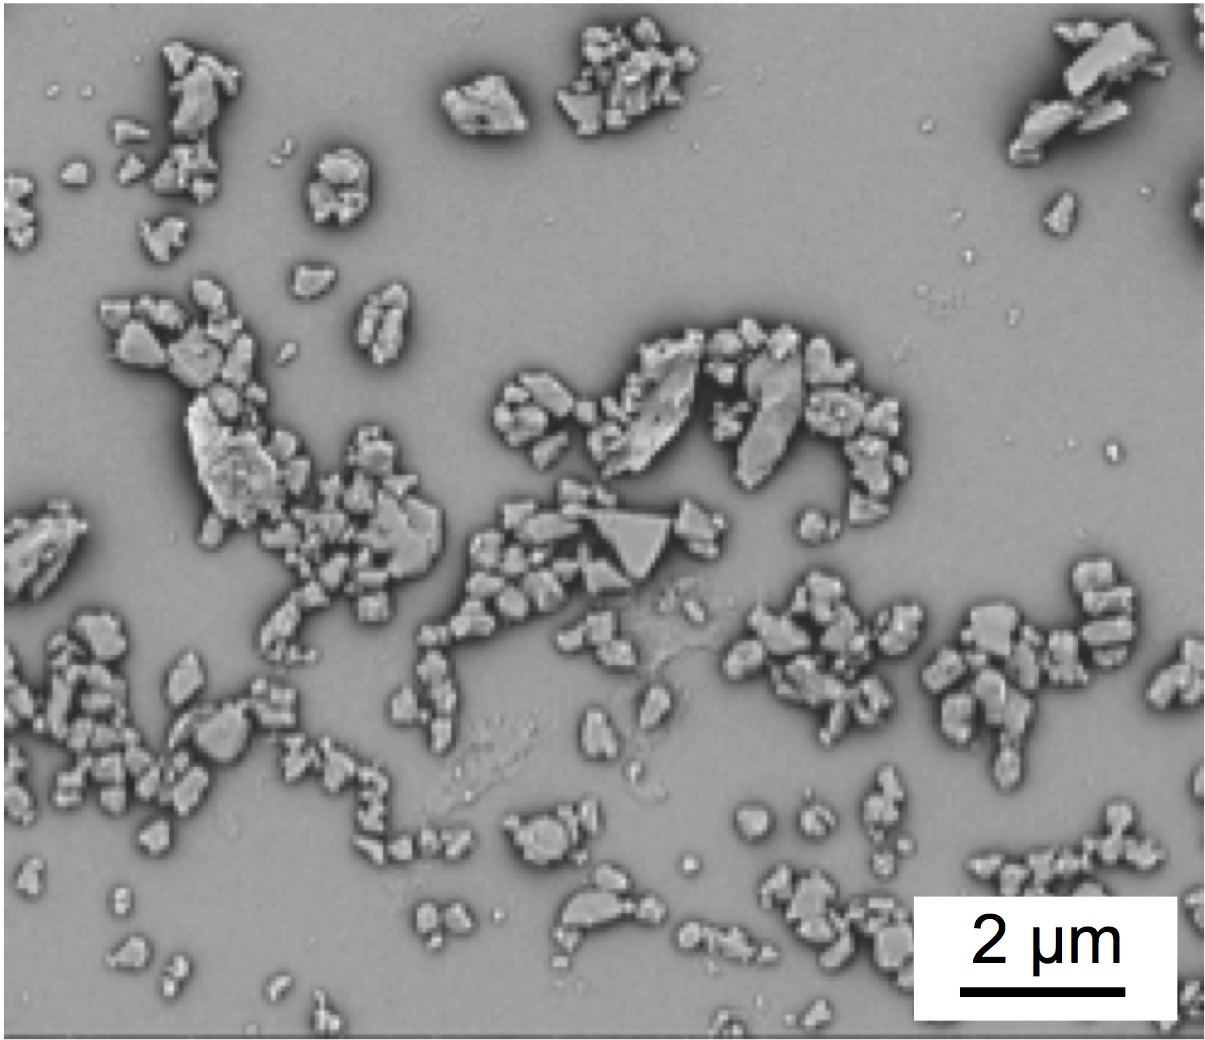
\includegraphics[width=\textwidth]{Chapter-3/Figures/Figure1.png}
	\caption{SEM image of 380 ppm MgO-doped specialty alumina powder used in this work.}
	\label{Ch3-figure:Figure1}
\end{figure}
%%%

\newpage
%%%
\begin{figure}[H]
	\centering
	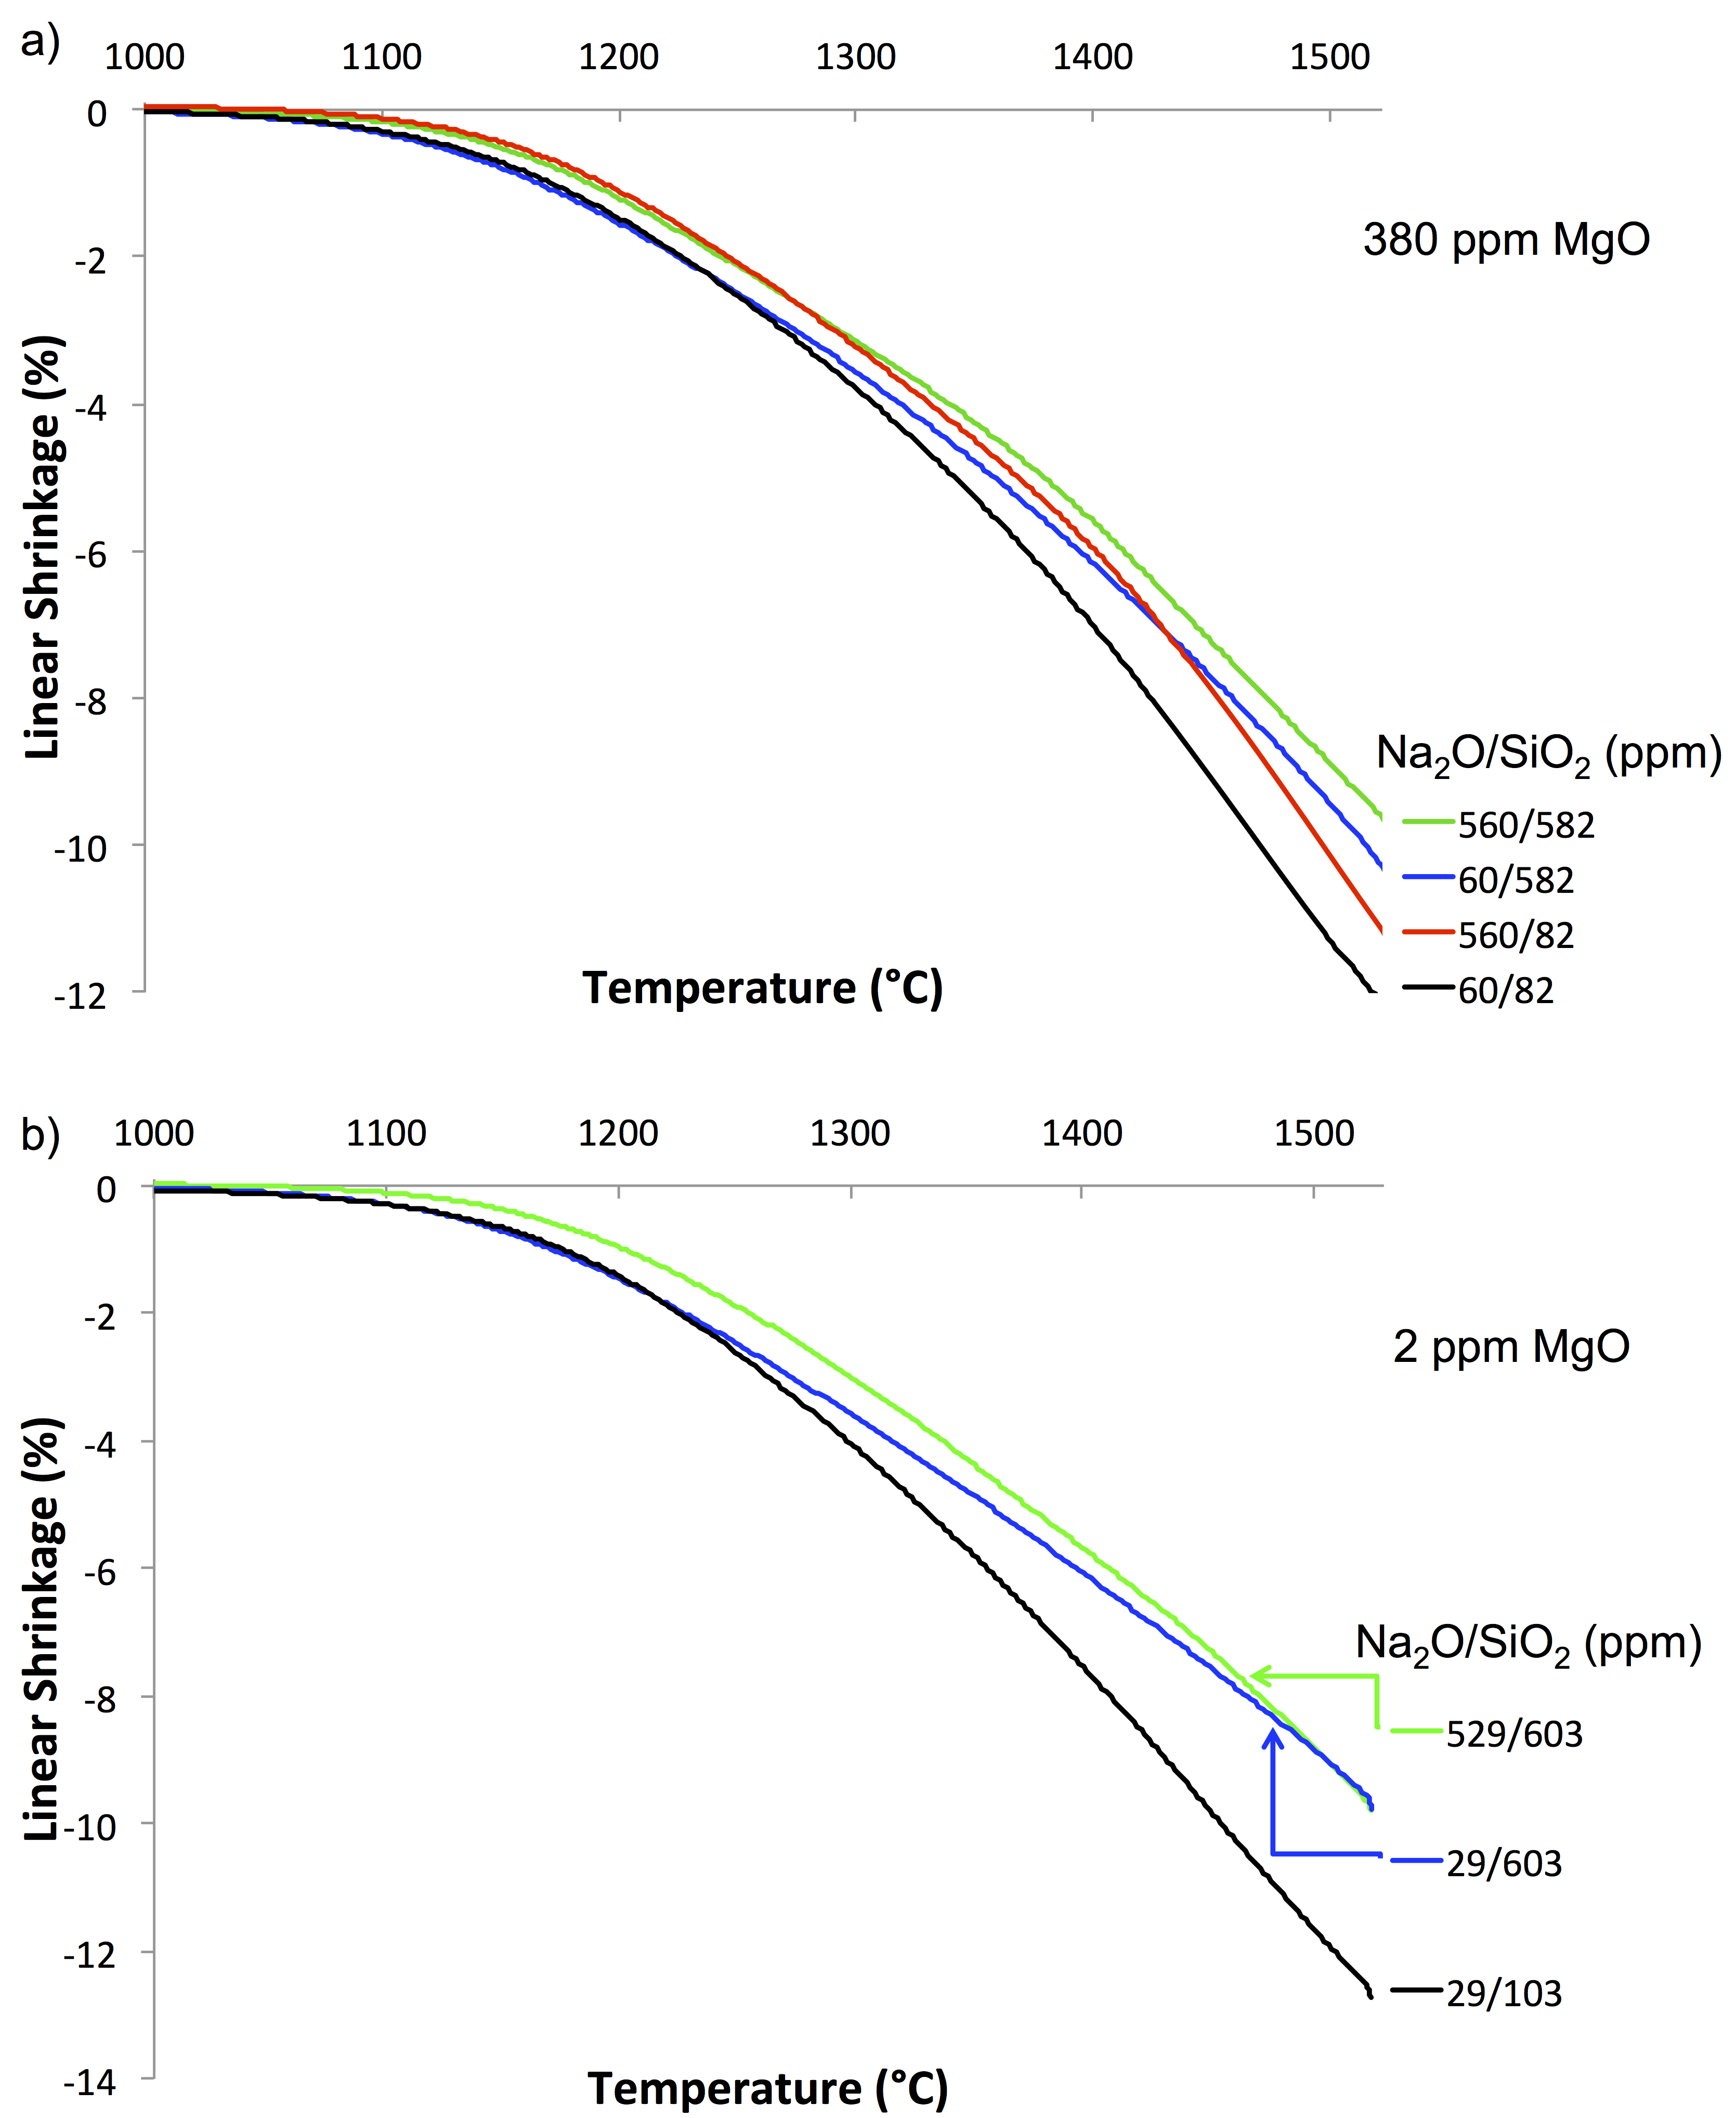
\includegraphics[width=\textwidth]{Chapter-3/Figures/Figure2.png}
	\caption{Dilatometer curves of a) 380 ppm MgO-doped and b) MgO-free \cite{Bae1997} specialty alumina samples with different Na$_{2}$O/SiO$_{2}$ levels heated at 10$^{\circ}$C/min to 1525$^{\circ}$C.}
	\label{Ch3-figure:Figure2}
\end{figure}
%%%

\newpage
%%%
\begin{figure}[H]
	\centering
	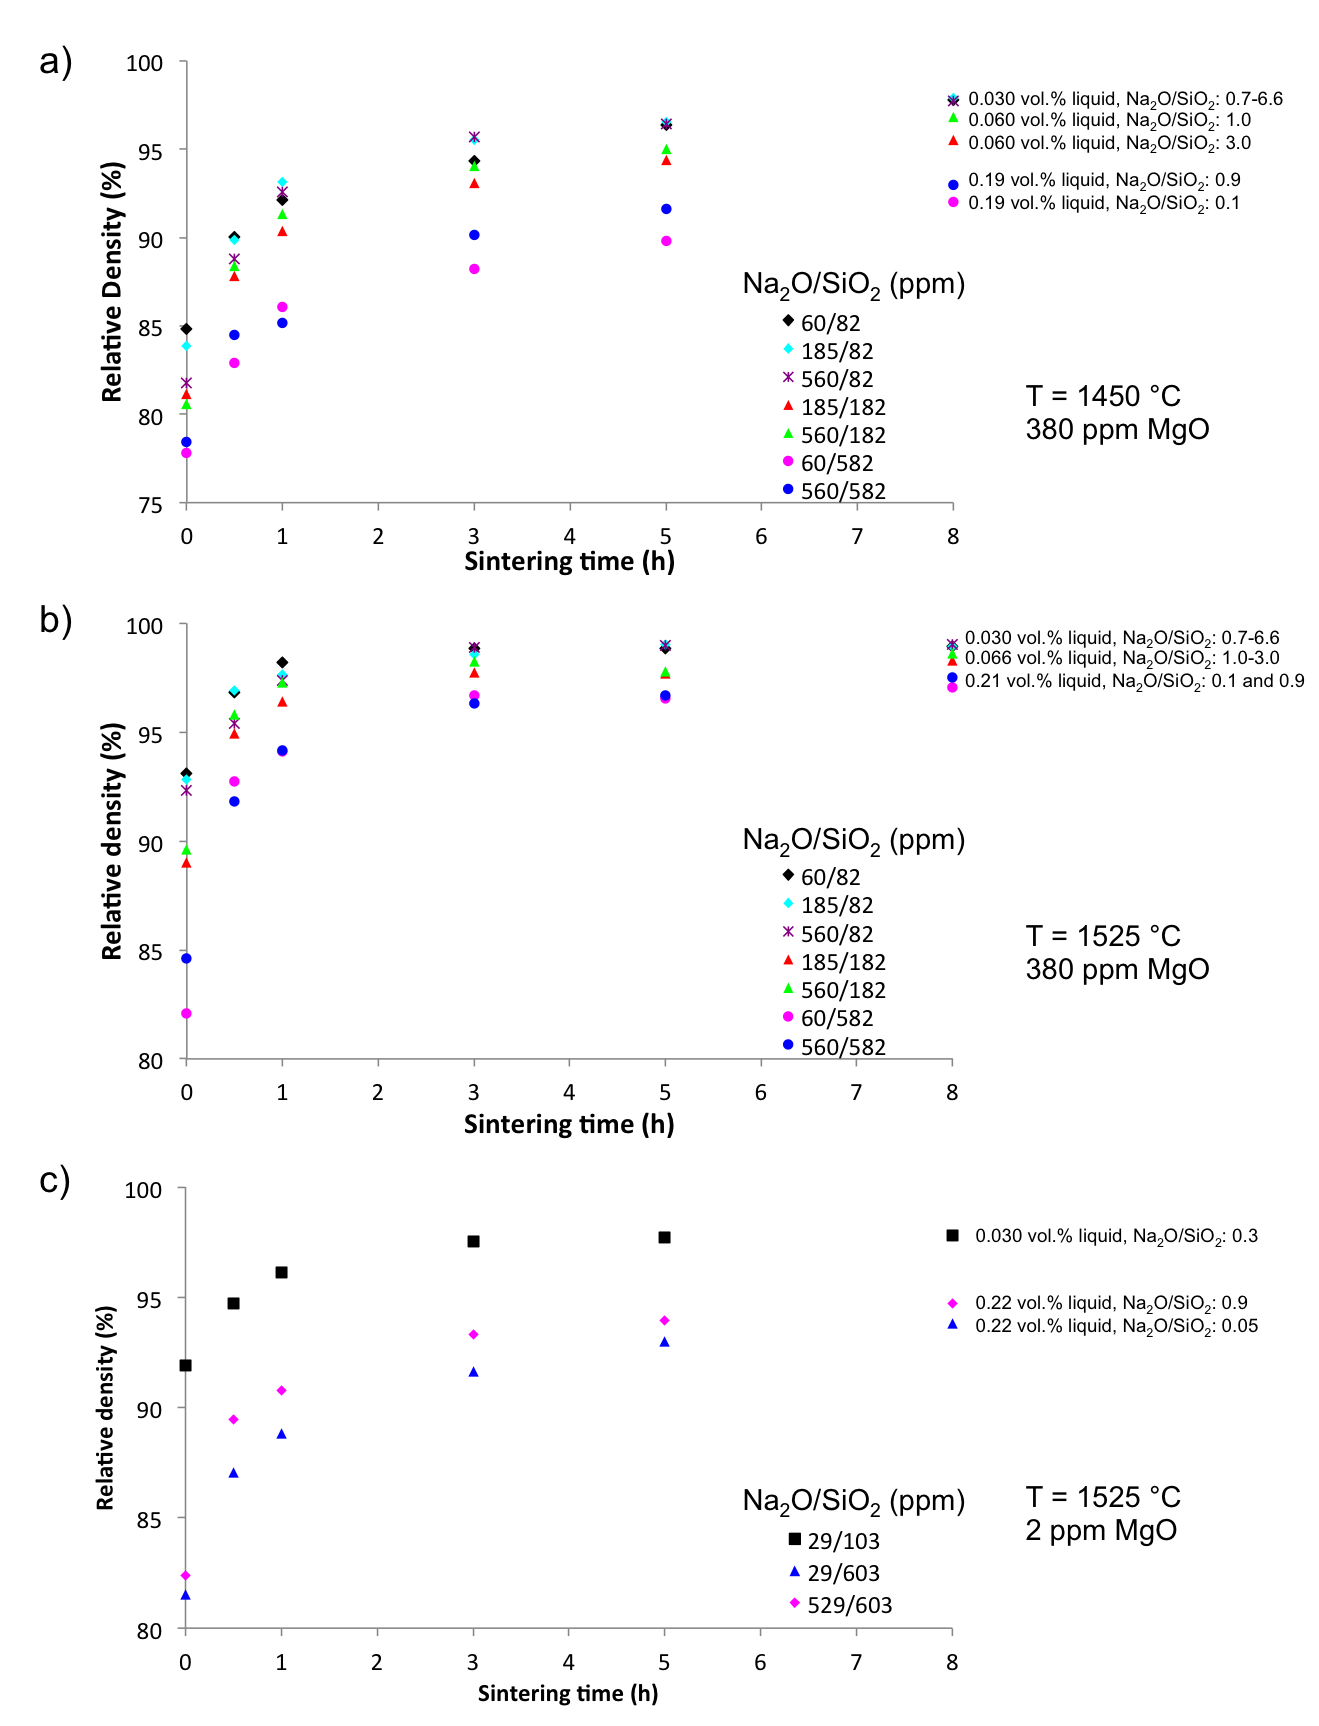
\includegraphics[width=\textwidth]{Chapter-3/Figures/Figure3.png}
	\caption{Densification kinetics of specialty processed alumina containing different amounts Na$_{2}$O and SiO$_{2}$ and a) 380 ppm MgO sintered at 1450$^{\circ}$C, b) 380 ppm MgO sintered at 1525$^{\circ}$C, and c) 2 ppm MgO sintered at 1525$^{\circ}$C \cite{Bae1997}.}
	\label{Ch3-figure:Figure3}
\end{figure}
%%%

\newpage
%%%
\begin{figure}[H]
	\centering
	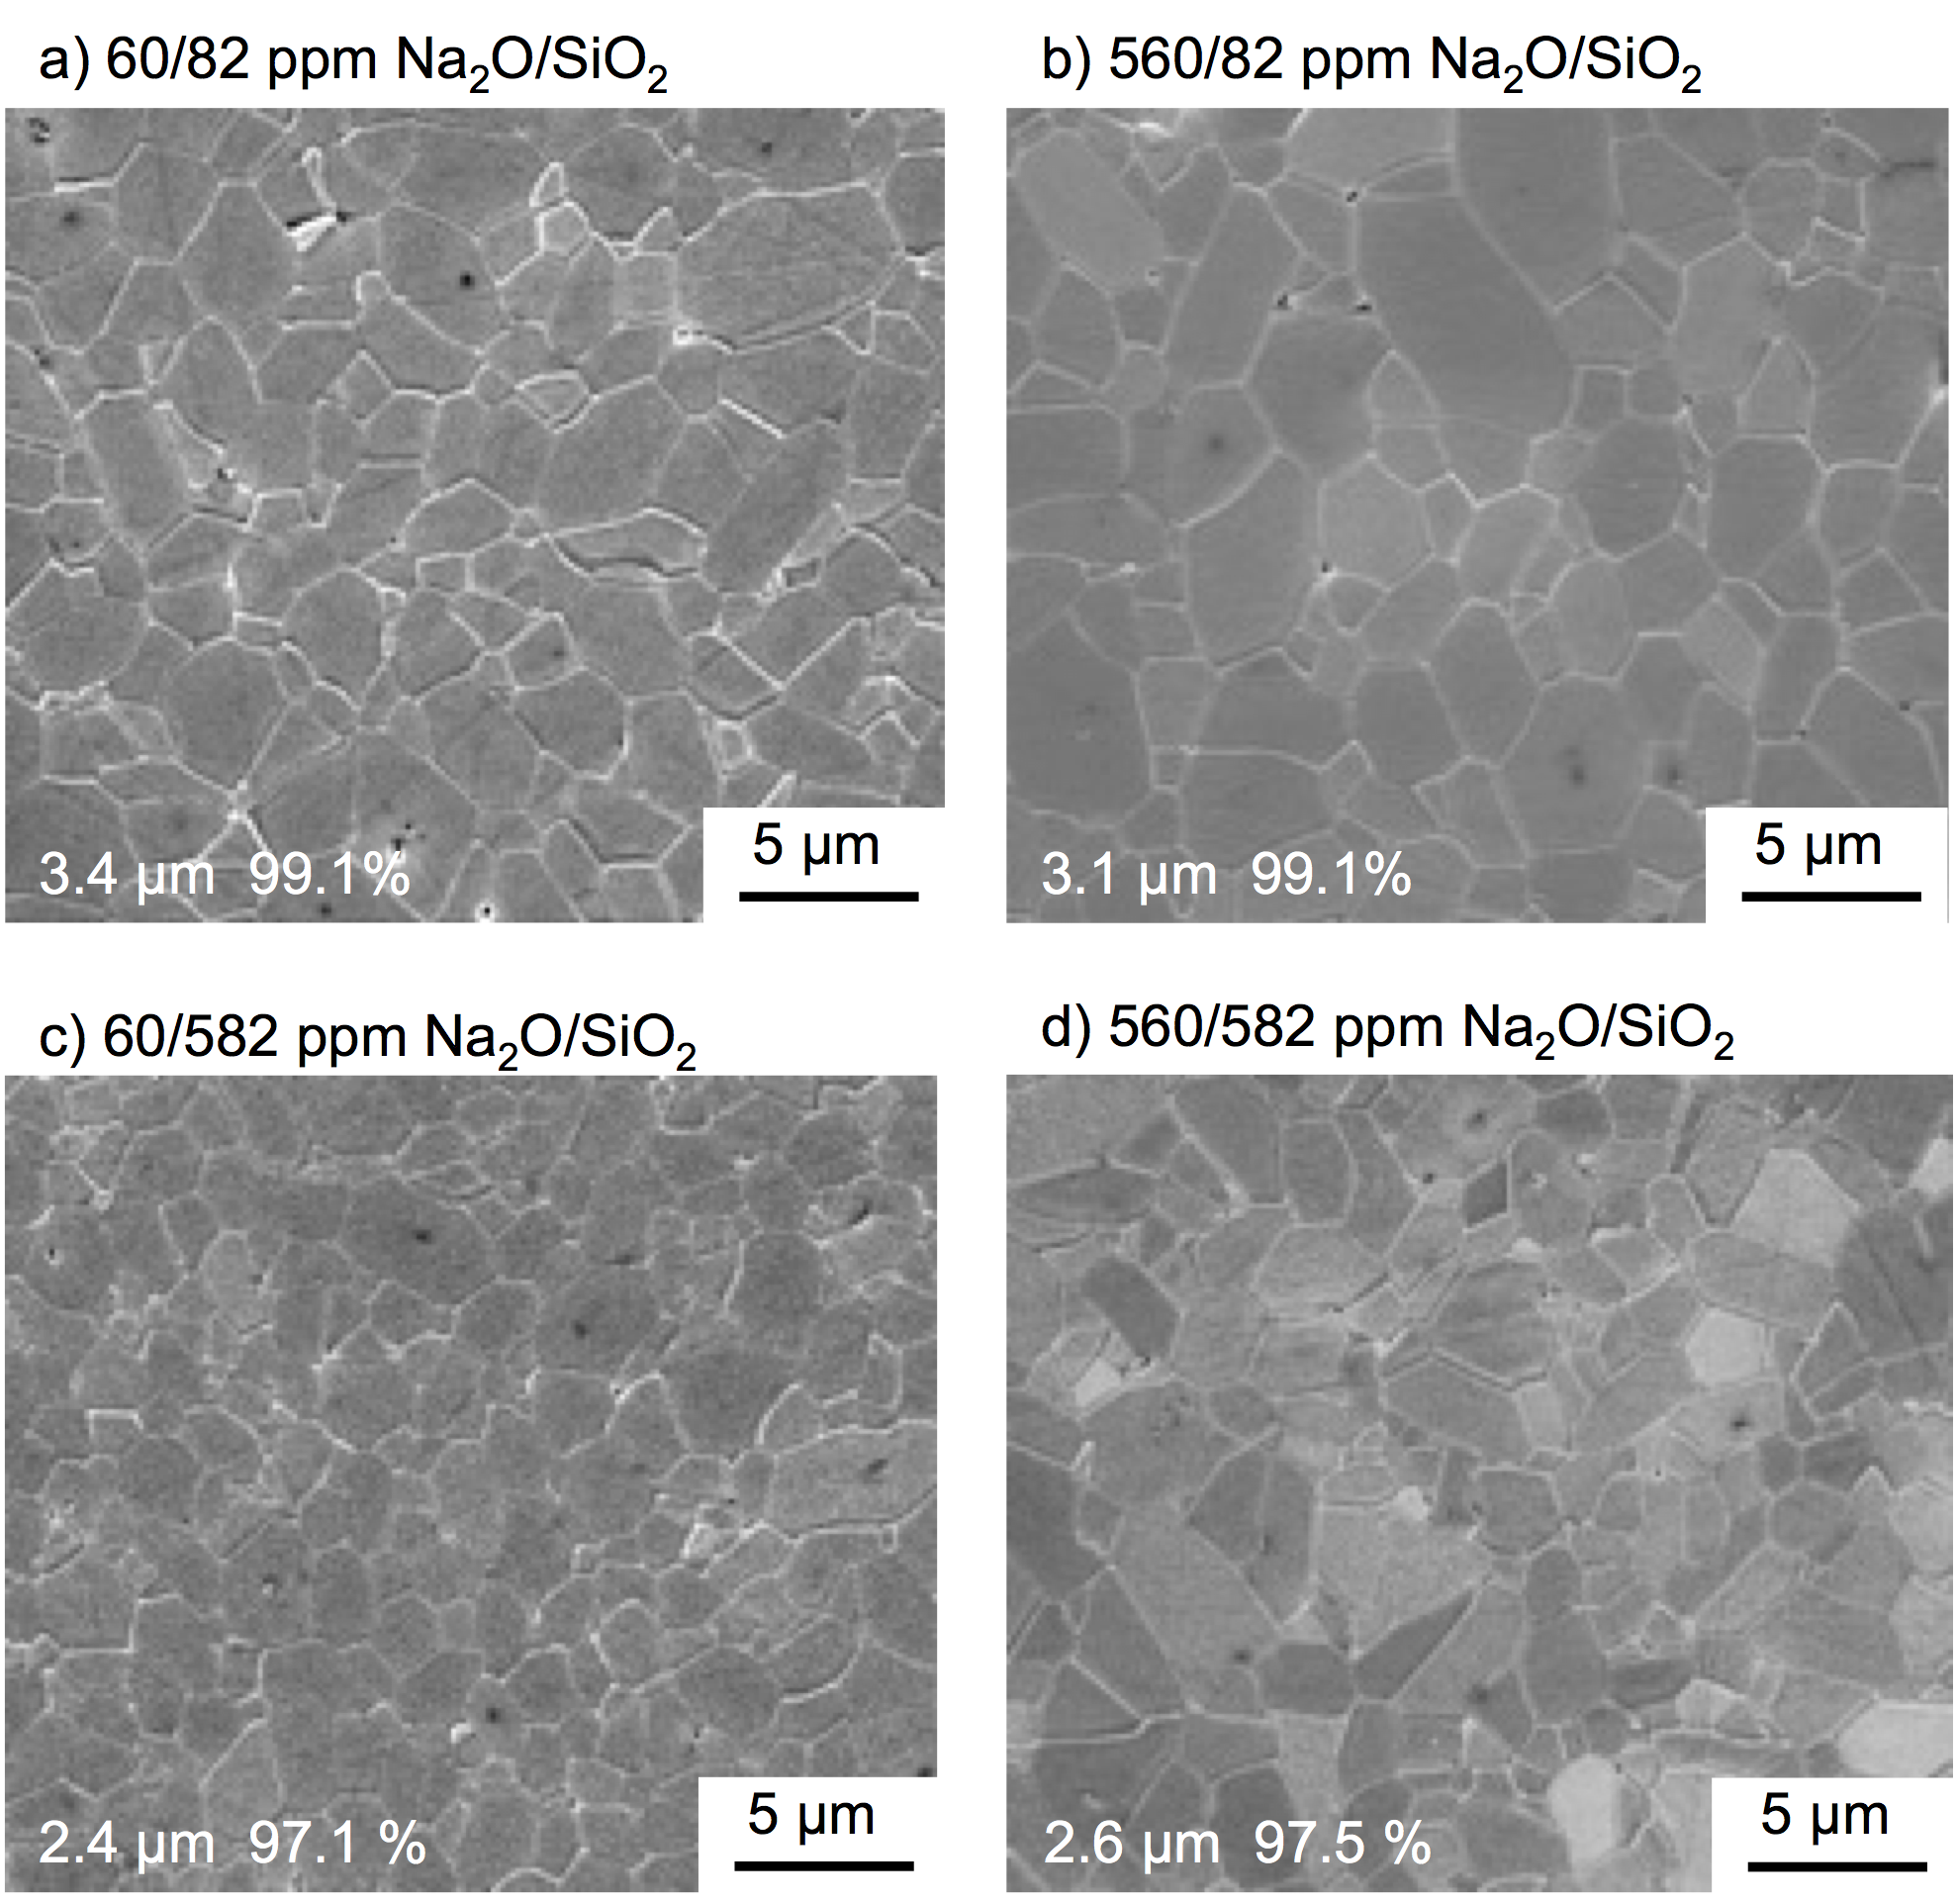
\includegraphics[width=\textwidth]{Chapter-3/Figures/Figure4.png}
	\caption{Microstructures of 380 ppm MgO-doped specialty alumina samples with different Na$_{2}$O and SiO$_{2}$ concentrations sintered at 1525$^{\circ}$C for 8 h.}
	\label{Ch3-figure:Figure4}
\end{figure}
%%%

\newpage
%%%
\begin{figure}[H]
	\centering
	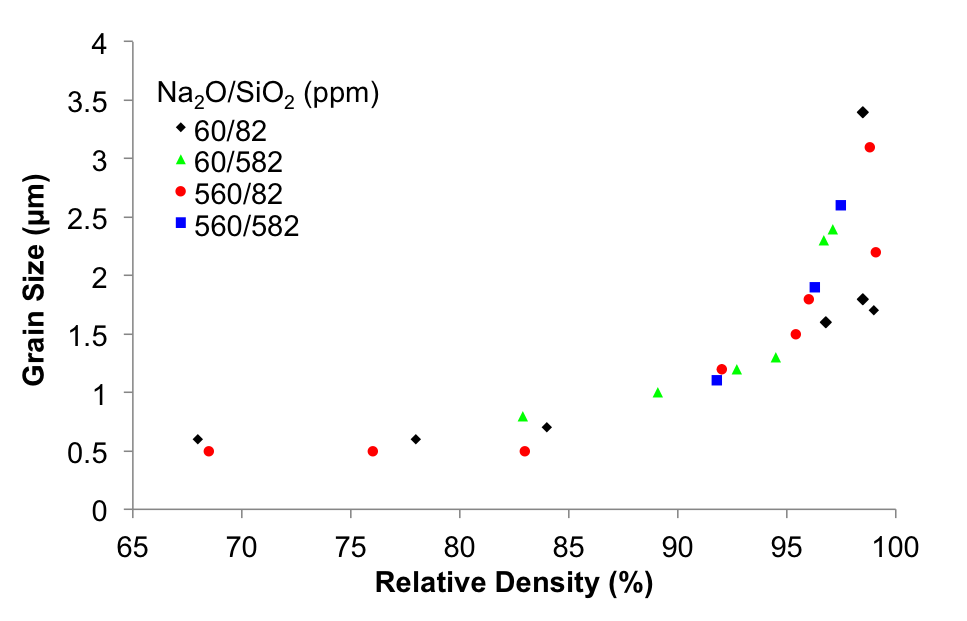
\includegraphics[width=\textwidth]{Chapter-3/Figures/Figure5.png}
	\caption{Sintering trajectories (grain size vs. relative density) for 380 ppm MgO-doped specialty alumina samples with different Na$_{2}$O and SiO$_{2}$ concentrations.}
	\label{Ch3-figure:Figure5}
\end{figure}
%%%

\newpage
%%%
\begin{figure}[H]
	\centering
	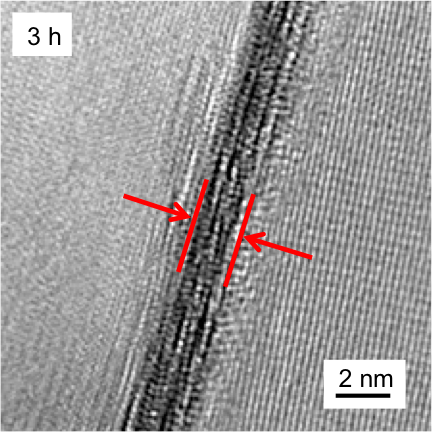
\includegraphics[width=\textwidth]{Chapter-3/Figures/Figure6.png}
	\caption{Grain boundary of a sample containing 529 ppm Na$_{2}$O, 603 ppm SiO$_{2}$, and 2 ppm MgO after 3 h at 1525$^{\circ}$C.}
	\label{Ch3-figure:Figure6}
\end{figure}
%%%

\newpage
%%%
\begin{figure}[H]
	\centering
	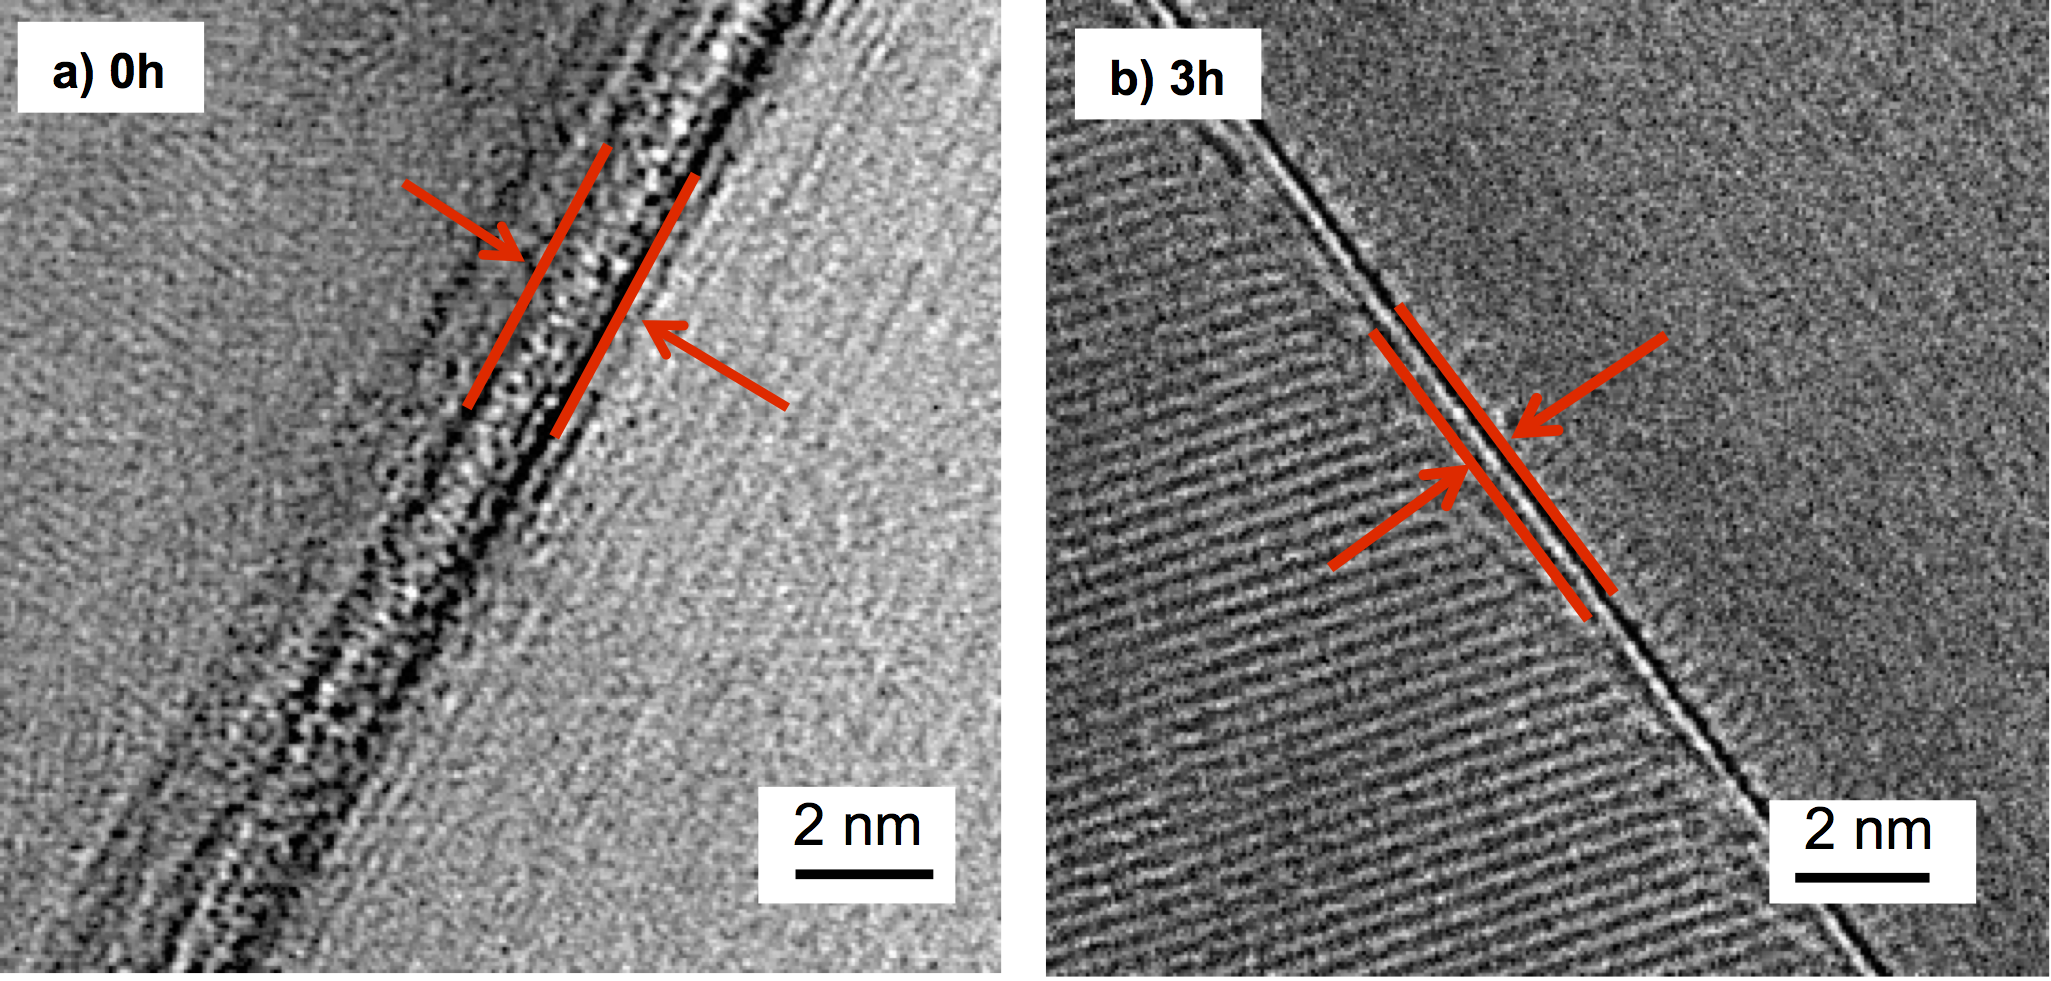
\includegraphics[width=\textwidth]{Chapter-3/Figures/Figure7.png}
	\caption{Grain boundaries of samples containing 560 ppm Na$_{2}$O, 582 ppm SiO$_{2}$, and 380 ppm MgO after a) 0 h and b) 3 h at 1525$^{\circ}$C.}
	\label{Ch3-figure:Figure7}
\end{figure}
%%%

\newpage
%%%
\begin{figure}[H]
	\centering
	\includegraphics[width=\textwidth]{Chapter-3/Figures/Figure8.png}
	\caption{EDS of grain boundaries of samples containing 560 ppm Na$_{2}$O, 582 ppm SiO$_{2}$, and 380 ppm MgO after a) 0 h and b) 3 h at 1525$^{\circ}$C showing the Si distribution. After 0 h Si shows a stronger segregation to the grain boundaries than after 3 h.}
	\label{Ch3-figure:Figure8}
\end{figure}
%%%

\newpage
%%%
\begin{figure}[H]
	\centering
	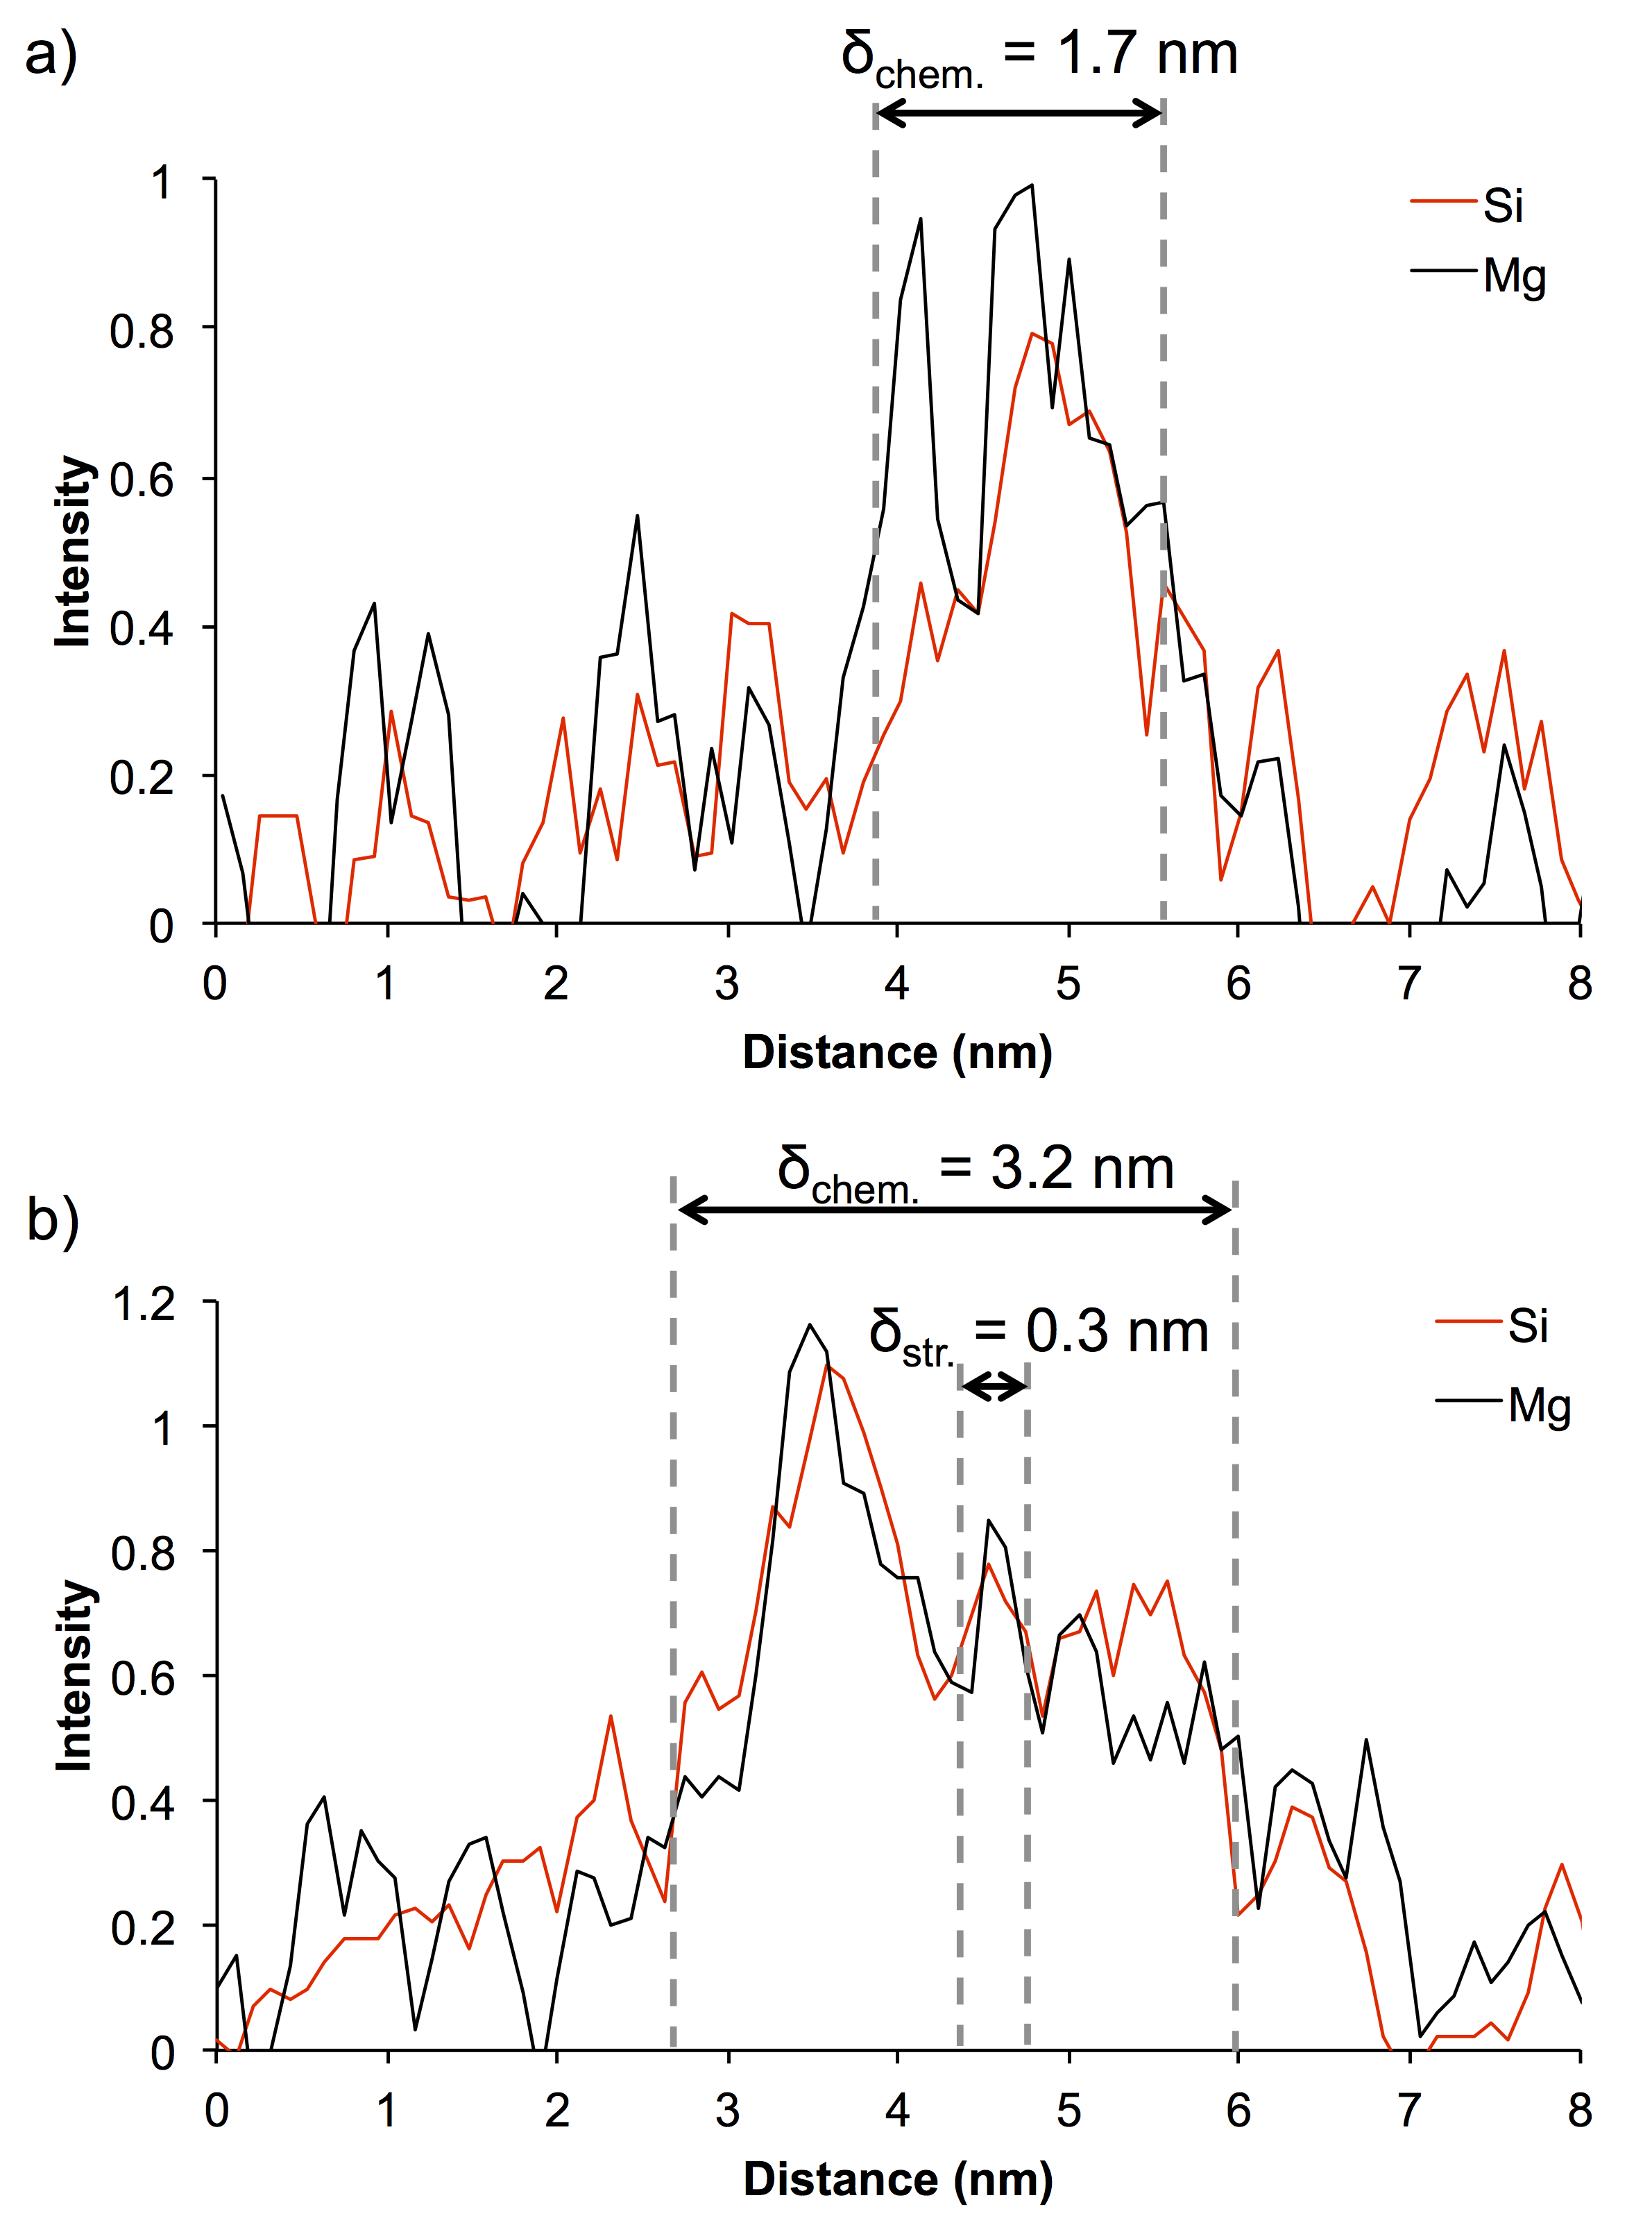
\includegraphics[width=\textwidth]{Chapter-3/Figures/Figure9.png}
	\caption{EDS line scan across a grain boundary of a sample containing 560 ppm Na$_{2}$O, 582 ppm SiO$_{2}$, and 380 ppm MgO after sintering at 1525$^{\circ}$C for a) 0 h and b) 3 h.}
	\label{Ch3-figure:Figure9}
\end{figure}
%%%

\newpage
%%%
\begin{figure}[H]
	\centering
	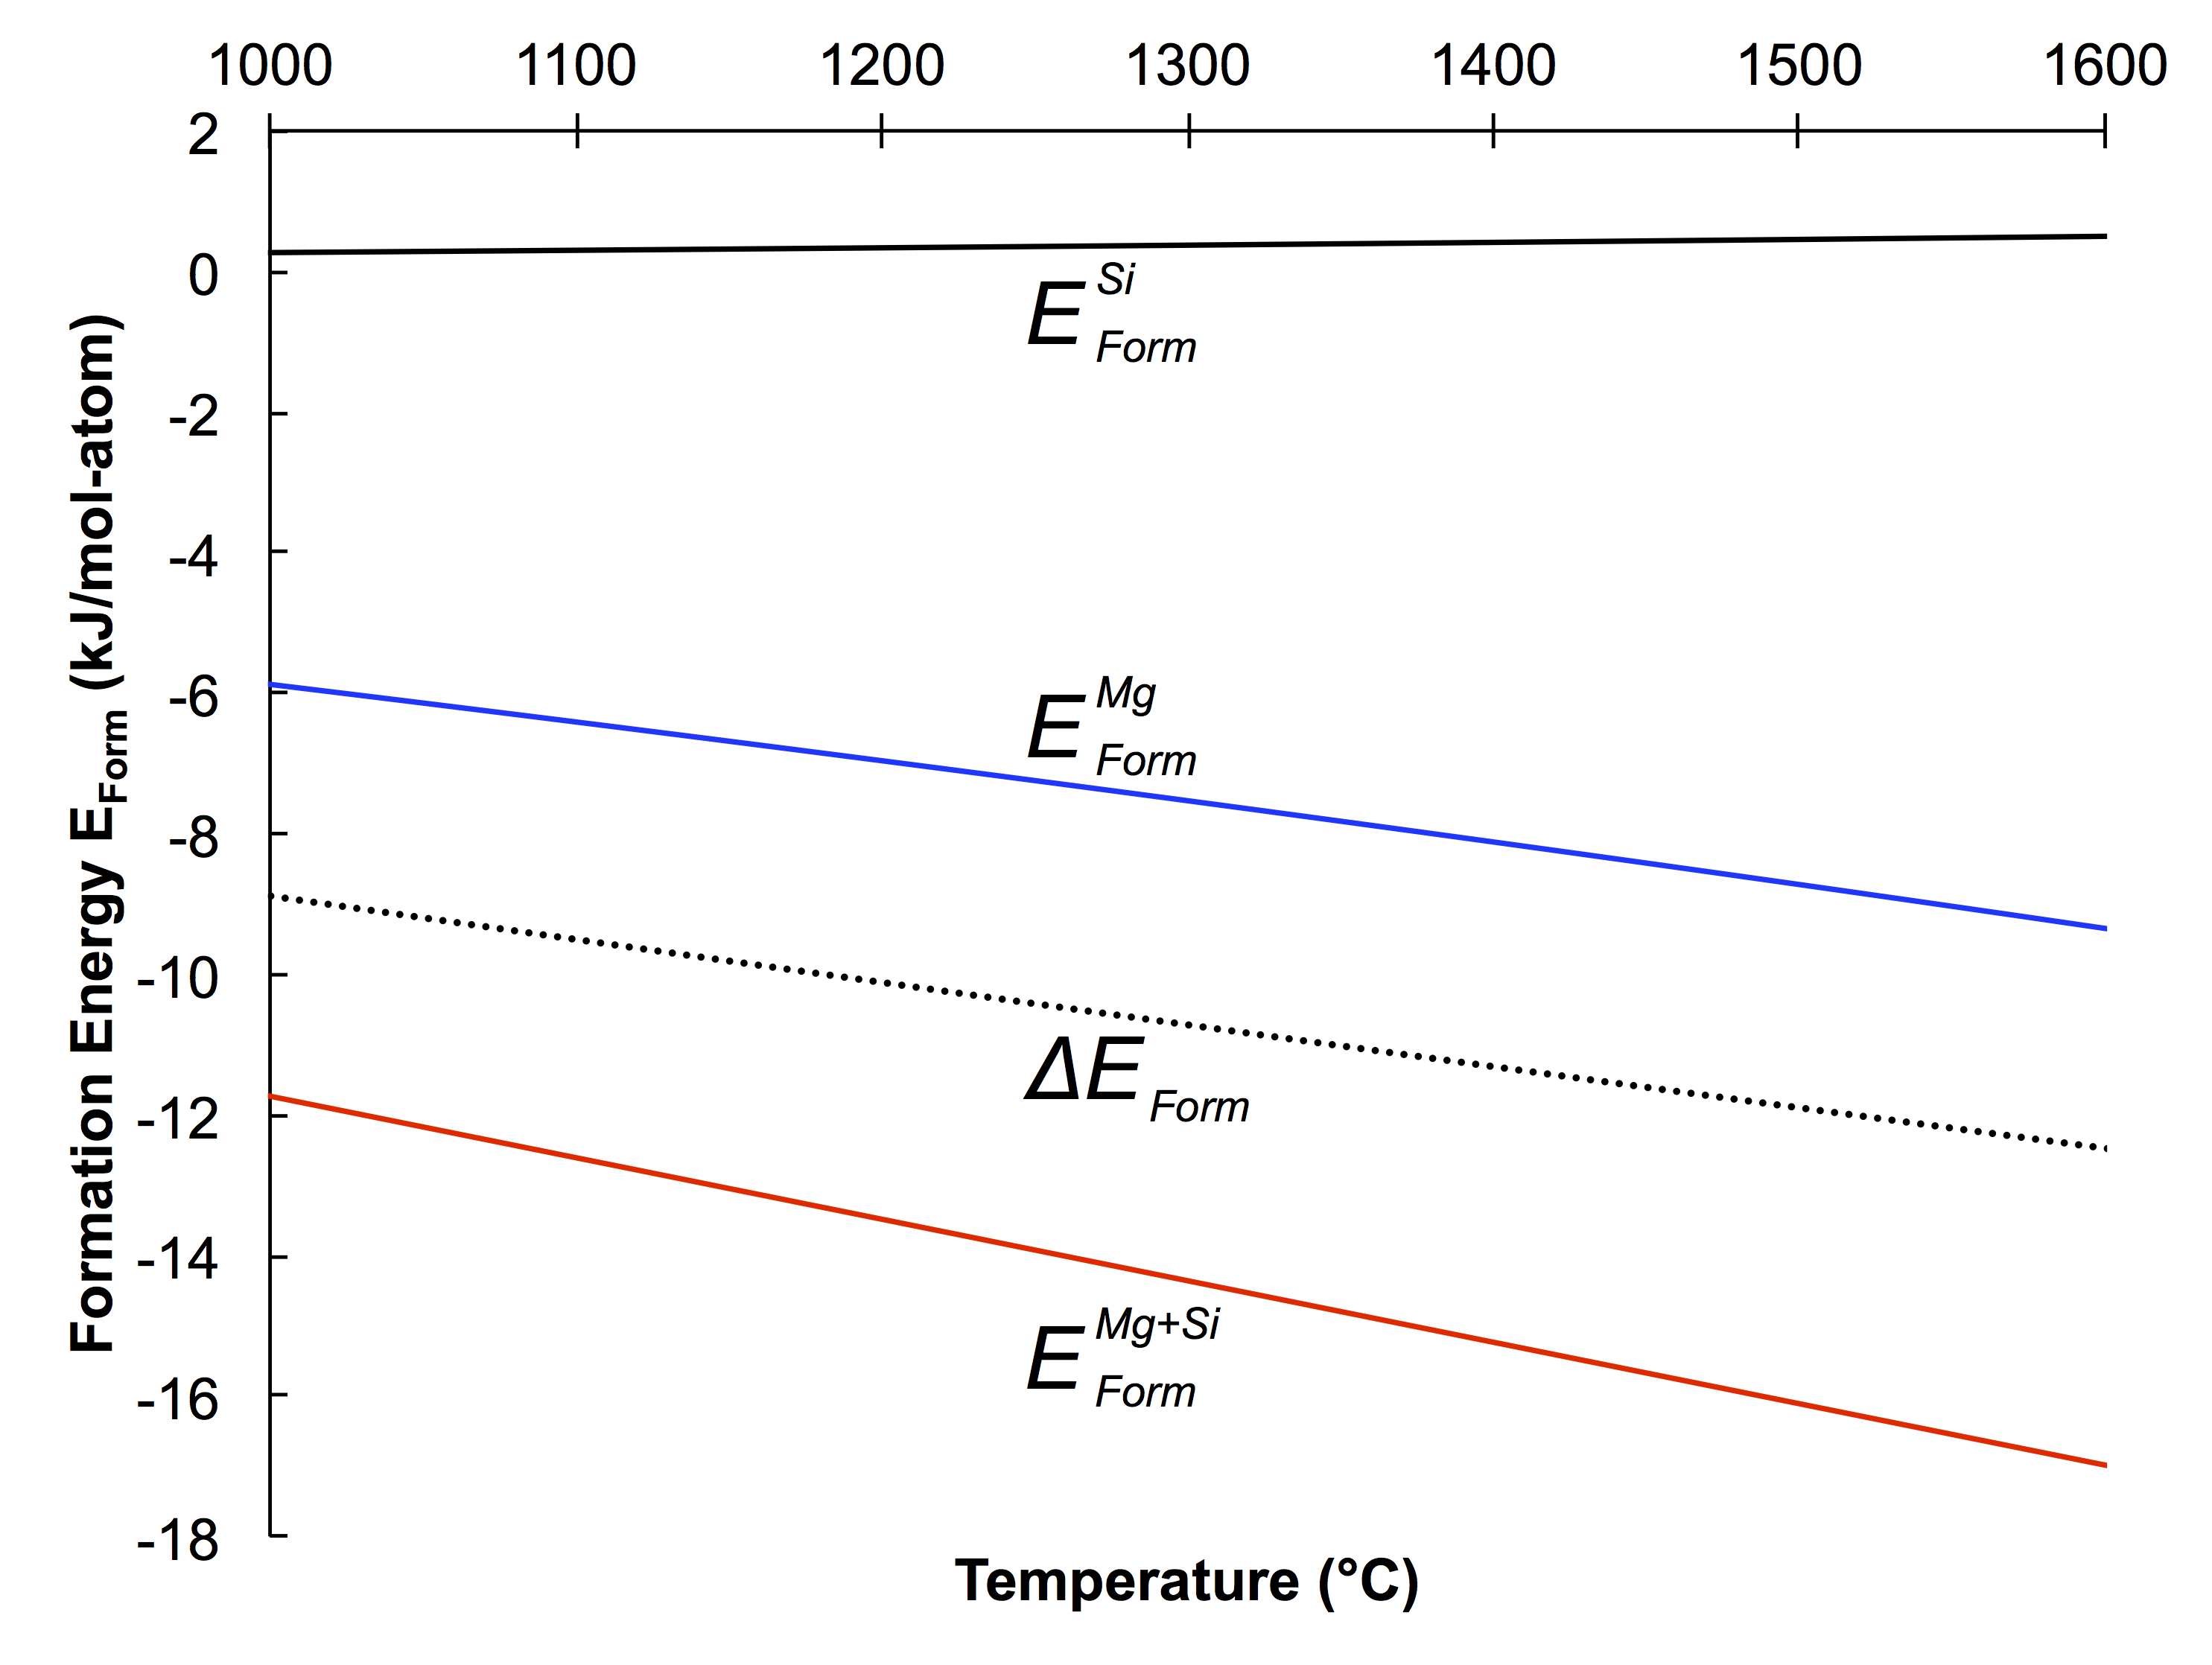
\includegraphics[width=\textwidth]{Chapter-3/Figures/Figure10.png}
	\caption{Comparison of the formation energy of alpha-Al$_{2}$O$_{3}$ with an Mg-cluster ($E_{Form}^{Mg}$), Si-cluster ($E_{Form}^{Si}$) and Mg+Si-cluster ($E_{Form}^{Mg+Si}$) as a function of temperature. The formation energy difference ($\bigtriangleup E_{Form}$) between the structures was calculated from Eq. REF to compare the formation energy values and show that it is energetically favorable to form Mg+Si-clusters over Si-clusters and Mg-clusters.}
	\label{Ch3-figure:Figure10}
\end{figure}
%%%

\newpage
%%%
\begin{figure}[H]
	\centering
	\includegraphics[width=\textwidth]{Chapter-3/Figures/Figure11.png}
	\caption{EDS maps of different oxides in 380 ppm MgO-doped specialty alumina samples after sintering at 1525$^{\circ}$C for a-d) 0 h and e-h) 3 h.}
	\label{Ch3-figure:Figure11}
\end{figure}
%%%

\newpage
%%%
\begin{figure}[H]
	\centering
	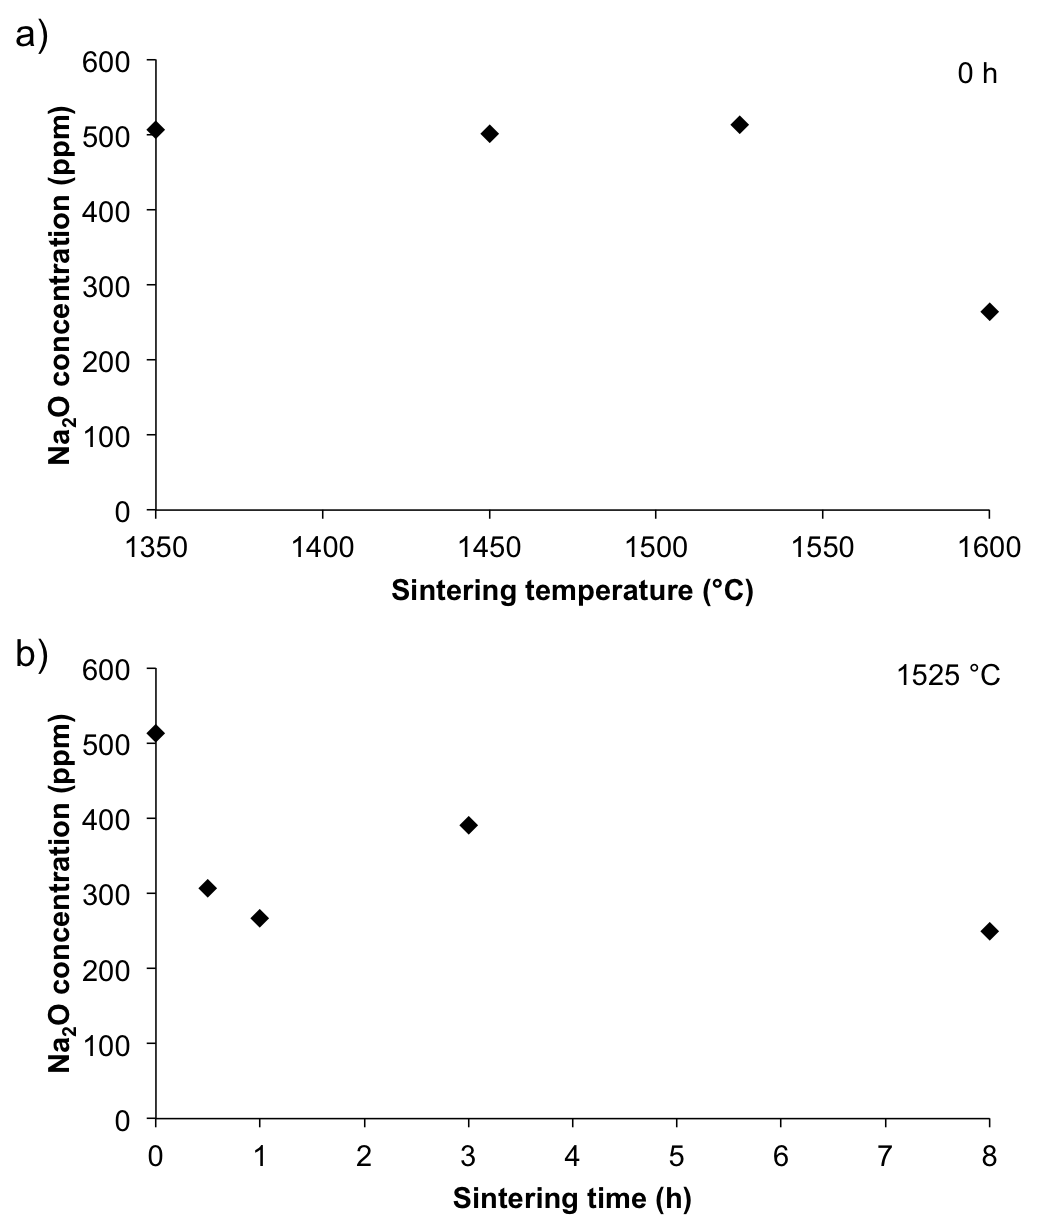
\includegraphics[width=\textwidth]{Chapter-3/Figures/Figure12.png}
	\caption{Na$_{2}$O concentration (ICP measurements) of 380 ppm MgO-doped specialty alumina samples with 560 ppm Na$_{2}$O as a) function of sintering temperature and b) as a function of sintering time at 1525 $^{\circ}$C.}
	\label{Ch3-figure:Figure12}
\end{figure}
%%%
\chapter{Powder Chemistry Effects on the Sintering Behavior of MgO-doped Bayer Alumina}

\section{Introduction}
When in the Course of human events, it becomes necessary for one people  to dissolve the political bands which have connected them with another,  and to assume among the powers of the earth, the separate and equal station  to which the Laws of Nature and of Nature's God entitle them, a decent respect to the opinions of mankind requires that they should declare  the causes which impel them to the separation.

\section{More Declaration}

We hold these truths to be self-evident, that all men are created equal,  that they are endowed by their Creator with certain unalienable Rights,  that among these are Life, Liberty and the pursuit of Happiness. --That to secure these  rights, Governments are instituted among Men, deriving their just powers  from the consent of the governed, --That whenever any Form of Government  becomes destructive of these ends, it is the Right of the People to alter  or to abolish it, and to institute new Government, laying its foundation on  such principles and organizing its powers in such form, as to them shall  seem most likely to effect their Safety and Happiness. Prudence, indeed, will dictate that Governments long established should not  be changed for light and transient causes; and accordingly all experience  hath shewn, that mankind are more disposed to suffer, while evils are  sufferable, than to right themselves by abolishing the forms to which they  are accustomed.

\subsection{Some nonsense here}

But when a long train of abuses and usurpations, pursuing invariably the same  Object evinces a design to reduce them under absolute Despotism, it is their  right, it is their duty, to throw off such Government, and to provide new Guards for their future security. --Such has been the patient sufferance of these Colonies; and such is now the  necessity which constrains them to alter their former Systems of Government.

\subsection{Some additional nonsense here}

The history of the present King of Great Britain [George III] is a history  of repeated injuries and usurpations, all having in direct object the  establishment of an absolute Tyranny over these States. To prove this, let Facts be submitted to a candid world.
\chapter{Second phase formation in Bayer alumina}

\section{Introduction}
It is reported in the literature that dopants and impurities such as MgO, CaO, and Na$_{2}$O can form second phases such as spinel, calcium hexaluminate, and $\beta$-Al$_{2}$O$_{3}$, respectively, if their concentration is high enough. For Bayer aluminas $\beta$-Al$_{2}$O$_{3}$ is of particular interest because Na$_{2}$O impurities are characteristic to Bayer alumina and small amounts of a few hundred ppm can be sufficient to form $\beta$-Al$_{2}$O$_{3}$. Rankin and Merwin \cite{Rankin1916} were the first to observe the formation of a new alumina phase in the high Al$_{2}$O$_{3}$ region in the system CaO-Al$_{2}$O$_{3}$-MgO. They believed it was an allotropic modification of Al$_{2}$O$_{3}$, and named it $\beta$-Al$_{2}$O$_{3}$. However, later work clarified that there is a relation between the alkali content in the Al$_{2}$O$_{3}$ and the formation of $\beta$-Al$_{2}$O$_{3}$ \cite{Stillwell1926}, and that $\beta$-Al$_{2}$O$_{3}$ is an alkali aluminate, rather than an allotropic form of Al$_{2}$O$_{3}$ \cite{Vries1969}. Ridgway et al. \cite{Ridgway1936} reported that the Na$_{2}$O content in Bayer process alumina can be high enough for the formation of $\beta$-Al$_{2}$O$_{3}$, and that $\beta$-Al$_{2}$O$_{3}$ forms in "dry ore process" Al$_{2}$O$_{3}$ (with unspecified low concentrations of Na$_{2}$O) only when Na$_{2}$O or K$_{2}$O is added. Four types of $\beta$-Al$_{2}$O$_{3}$ exist; two of them, $\beta$-Al$_{2}$O$_{3}$ (Na$_{2}$O*11Al$_{2}$O$_{3}$) and $\beta$''-Al2O3 (Na2O.5Al2O3), form in the binary system Na$_{2}$O-Al$_{2}$O$_{3}$, and can incorporate MgO. The other two beta aluminas, $\beta$'''-Al$_{2}$O$_{3}$ and $\beta$''''-Al$_{2}$O$_{3}$ are found in the ternary system Na$_{2}$O-Al$_{2}$O$_{3}$-MgO \cite{Stevens1984}. For completeness it should be mentioned that the existence of a $\beta$'-Al$_{2}$O$_{3}$ (Na$_{2}$O*7Al$_{2}$O$_{3}$) has been reported as well, but subsequent literature is in agreement that $\beta$'-Al$_{2}$O$_{3}$ is actually $\beta$-Al$_{2}$O$_{3}$ with excess Na$_{2}$O \cite{Stevens1984}.

The formation and stability of $\beta$-Al$_{2}$O$_{3}$ has been extensively studied in the literature because its excellent ion conductivity makes it suitable for applications as a solid electrolyte; especially for use in batteries. Most reported preparation routs involve sodium carbonate and alumina \cite{Vries1969,Kummer1972a,Ray1975}. Heating mixtures of alumina and sodium carbonate to 1100$^{\circ}$C leads to the formation of $\beta$''-Al$_{2}$O$_{3}$, which decomposes to $\beta$-Al$_{2}$O$_{3}$ and NaAlO$_{2}$ at temperatures >1500$^{\circ}$C. The equilibrium vapor pressure of Na$_{2}$O over $\beta$-Al$_{2}$O$_{3}$ has been reported to be "appreciable" at temperatures >1400$^{\circ}$C \cite{Kummer1972a}, where $\beta$-Al$_{2}$O$_{3}$ can decompose to $\alpha$-Al$_{2}$O$_{3}$ by volatilization of Na$_{2}$O. However, soda loss has been reported to occur at lower temperatures as well, e.g. 6.4 wt\% of soda loss was reported by de Vries and Roth \cite{Vries1969} when they prepared $\beta$''-alumina samples and heated it for 4 h at 1100 $^{\circ}$C. On the other hand, Gallup \cite{Gallup1935} investigated the stability of $\beta$-Al$_{2}$O$_{3}$ at high temperatures and under different atmospheres and he reported that $\beta$-Al$_{2}$O$_{3}$ can convert to $\alpha$-Al$_{2}$O$_{3}$ at temperatures as low as 1300$^{\circ}$C in hydrogen or vacuum atmosphere, but in air no conversion was observed for heating as long as 1 h at 1500$^{\circ}$C. Full conversion was observed when the material was heated for 10 min at 1600$^{\circ}$C.

Even though the conditions for the formation of $\beta$-Al$_{2}$O$_{3}$ in $\alpha$-Al$_{2}$O$_{3}$ ceramics are of great importance, especially because the Na$_{2}$O content in Bayer process Al$_{2}$O$_{3}$ is sufficient for the formation of $\beta$-Al$_{2}$O$_{3}$, it is barely studied in literature. Duncan and Creyke \cite{Duncan1969a} investigated the formation and stability of $\beta$-Al$_{2}$O$_{3}$ in $\alpha$-Al$_{2}$O$_{3}$ ceramics and used two commercial alumina powders with impurities of 0.038 wt\% SiO$_{2}$, 0.006 wt\% MgO and 0.061 ppm Na$_{2}$O, and 0.04 wt\% SiO$_{2}$, 0.2 wt\% MgO and 0.04 wt\% Na$_{2}$O, respectively. They reported that $\beta$-Al$_{2}$O$_{3}$ can form at Na$_{2}$O concentrations as low as 300 ppm if a small amount of MgO is present. They estimated the amount of $\beta$-Al$_{2}$O$_{3}$ by measuring the dielectric loss of the sample, since $\beta$-Al$_{2}$O$_{3}$ was observed to increase the dielectric loss of $\alpha$-Al$_{2}$O$_{3}$ samples. An increase in amount of $\beta$-Al$_{2}$O$_{3}$ was observed with increasing Na$_{2}$O, but also with increasing MgO additions, and it was shown by electron-probe microanalysis that there is a higher concentration of Na$_{2}$O and MgO in the $\beta$-Al$_{2}$O$_{3}$ grains. They state that samples, in which $\beta$-Al$_{2}$O$_{3}$ forms, show no formation of spinel \cite{Duncan1969a} and furthermore they determined that $\beta$-Al$_{2}$O$_{3}$ in $\alpha$-Al$_{2}$O$_{3}$ is stable to up to 1650 $^{\circ}$C in stagnant air. In a flowing air stream, however, decomposition to $\alpha$-Al$_{2}$O$_{3}$ takes place, even in the center of the sample and the decomposition is facilitated by open porosity and higher temperatures, whereas a high degree of compaction of the powder, e.g. a high green density, impedes the decomposition. Small amounts of other oxides (e.g. SiO$_{2}$, MgO, ZrO$_{2}$) are reported to facilitate the decomposition process due to an easier diffusion path through the grain boundaries. The work by Duncan and Creyke focuses on the decomposition and while some literature reports indicate under what conditions $\beta$-Al$_{2}$O$_{3}$ may form \cite{Duncan1969a}, there is no systematic study on the formation of $\beta$-Al$_{2}$O$_{3}$ as function of powder chemistry, at what sintering stage $\beta$-Al$_{2}$O$_{3}$ forms and what possible formation mechanisms are. Goal of this work is to identify the stages and mechanisms of $\beta$-Al$_{2}$O$_{3}$ formation in $\alpha$-Al$_{2}$O$_{3}$.


\section{Experimental}

The samples fabricated for the investigations in Chapters 2 and 3 were used to investigate the formation of $\beta$-Al$_{2}$O$_{3}$ in $\alpha$-Al$_{2}$O$_{3}$. To investigate the influence of MgO concentration on the formation of $\beta$-Al$_{2}$O$_{3}$ the MgO-free powder used in Chaper 2 was also doped with up to 1000 ppm MgO using magnesium nitrate hexahydrate (Mg(NO$_{3}$)$_{2}$*6H$_{2}$O, 99.97\%, Alfa Aesar, Ward Hill, MA, USA). The alumina powder was dispersed in aqueous magnesium nitrate solution and stirred on a magnetic stir plate for 5 h at room temperature, and then held at 80 $^{\circ}$C for 24 h until the mixture was too viscous to stir. The mixture was then placed in a drying oven at 100 $^{\circ}$C for 24 h to thoroughly dry the powder. Additionally, an ultra-high purity powder (AKP-50, Sumitomo Chemical Co. Ltd., Tokyo, Japan) was doped with up to 2000 ppm Na$_{2}$O, 500 ppm SiO$_{2}$, and 500 ppm MgO and used to dry press samples. The intrinsic impurities in the ultra high purity powder are 11 ppm SiO$_{2}$, 4 ppm Fe2O3, 2 ppm Na$_{2}$O, 2 ppm MgO, and 1 ppm Cu. The doping and sample preparation procedure is described in detail in chapters 2 and 3.

\section{Results}

Initially the detection of $\beta$-Al$_{2}$O$_{3}$ in an $\alpha$-Al$_{2}$O$_{3}$ matrix was investigated. Figure \ref{Ch5-figure:Figure1}a-c shows SEM micrographs of $\beta$-Al$_{2}$O$_{3}$ grains in a sample with 529 ppm Na$_{2}$O, 103 ppm SiO$_{2}$, and 380 ppm MgO sintered at 1525$^{\circ}$C for 3 h. It can be seen that in unetched samples $\beta$-Al$_{2}$O$_{3}$ grains can hardly be observed in images obtained from secondary electrons (Figure \ref{Ch5-figure:Figure1}a). Figure \ref{Ch5-figure:Figure1}b shows an SEM image of the same area of the sample as Figure \ref{Ch5-figure:Figure1}a obtained from the backscattered electrons and a stronger contrast between the $\beta$-Al$_{2}$O$_{3}$ grains and the surrounding $\alpha$-Al$_{2}$O$_{3}$ matrix can be seen, which is due to the higher sensitivity of backscattered electrons to density. $\beta$-Al$_{2}$O$_{3}$ grains appear darker due to the lower density (3.31 g/cm$^{3}$) compared to $\alpha$-Al$_{2}$O$_{3}$ (3.986 g/cm$^{3}$). Figure \ref{Ch5-figure:Figure1}c shows a $\beta$-Al$_{2}$O$_{3}$ grain after thermal etching at 1425$^{\circ}$C for 40 min and it can be seen that the $\beta$-Al$_{2}$O$_{3}$ grain has evaporated during thermal etching, leaving a platelet shaped hole in the etched microstructure. It is interesting to note that samples with low Na$_{2}$O concentrations such as 29 ppm form $\beta$-Al$_{2}$O$_{3}$ grains that do not evaporate during thermal etching, as seen in Figure \ref{Ch5-figure:Figure1}d. SEM micrographs obtained from backscattered electrons were used to detect $\beta$-Al$_{2}$O$_{3}$ grains for the following investigations.

\subsection{Influence of MgO on the formation of $\beta$-Al$_{2}$O$_{3}$}

Figure \ref{Ch5-figure:Figure2}a shows the influence of MgO concentration on the number of $\beta$-Al$_{2}$O$_{3}$ grains after sintering at 1525$^{\circ}$C for 3 h. It can be seen that for a MgO concentration of 2 ppm no $\beta$-Al$_{2}$O$_{3}$ was observed, and with increasing the MgO concentration the number of $\beta$-Al$_{2}$O$_{3}$ grains that form increases up to 502 ppm MgO, but does not increase further when the MgO concentration is increased to 1002 ppm. This shows that MgO assists the formation of $\beta$-Al$_{2}$O$_{3}$. The influence of Na2O concentration on the number of $\beta$-Al$_{2}$O$_{3}$ grains in MgO-free Bayer alumina after sintering at 1525$^{\circ}$C for 3 h is shown in Figure \ref{Ch5-figure:Figure2}b. It can be seen that only a small number of $\beta$-Al$_{2}$O$_{3}$ grains form for concentrations $\leq$ 529 ppm Na2O, but for higher concentrations, such as 1029 ppm, the number of $\beta$-Al$_{2}$O$_{3}$ grains increases significantly. Since commercial Bayer aluminas are typically doped with MgO, the following investigations are focused on Bayer alumina powder that was doped with 380 ppm MgO.

\subsection{MgO-doped Bayer alumina}
\subsubsection{Number frequency of $\beta$-Al$_{2}$O$_{3}$ grains}

Figure \ref{Ch5-figure:Figure3} shows the influence of the Na$_{2}$O and SiO$_{2}$ concentration on the number density of $\beta$-Al$_{2}$O$_{3}$ grains in Bayer alumina powder doped with 380 ppm MgO. It can be seen that the number density of $\beta$-Al$_{2}$O$_{3}$ grains increases with increasing Na$_{2}$O concentration (Figure \ref{Ch5-figure:Figure3}a), but decreases as a function of SiO$_{2}$ concentration in samples with different Na$_{2}$O concentrations (Figure \ref{Ch5-figure:Figure3}b). This indicates that the Na$_{2}$O/SiO$_{2}$ ratio determines the number density of $\beta$-Al$_{2}$O$_{3}$ grains. Figure \ref{Ch5-figure:Figure3}c shows the number density of $\beta$-Al$_{2}$O$_{3}$ grains as a function of the Na$_{2}$O/SiO$_{2}$ ratio, and it can be seen that the number density of $\beta$-Al$_{2}$O$_{3}$ grains increases linearly with increasing Na$_{2}$O/SiO$_{2}$ ratio. 

The kinetics of $\beta$-Al$_{2}$O$_{3}$ formation at 1525$^{\circ}$C for different powder chemistries (MgO-doped Bayer alumina) is shown in Figure \ref{Ch5-figure:Figure4}. Most $\beta$-Al$_{2}$O$_{3}$ grains forms within the first hour at 1525$^{\circ}$C, and after that the number density of $\beta$-Al$_{2}$O$_{3}$ grains does not change for all chemistries. In contrast, for samples prepared from ultra high purity powder (AKP-50) the amount of $\beta$-Al$_{2}$O$_{3}$ that forms during sintering in the temperature range from 1450$^{\circ}$C to 1600$^{\circ}$C for up to 8 h does not change, regardless of the Na$_{2}$O, MgO, or SiO$_{2}$ concentrations. However, in the ultra-high purity powder it was observed that increasing the Na$_{2}$O and MgO concentrations increases the number of $\beta$-Al$_{2}$O$_{3}$ grains in the microstructures, and increasing the SiO$_{2}$ concentration decreases the number of $\beta$-Al$_{2}$O$_{3}$ grains in the microstructures, similar to the Bayer alumina powder.

\subsubsection{Size of $\beta$-Al$_{2}$O$_{3}$ grains}
Figure \ref{Ch5-figure:Figure5} shows micrographs of samples with different powder chemistries with up to 1000 ppm MgO, Na$_{2}$O, and SiO$_{2}$ after sintering at 1525$^{\circ}$C for 3 h. It can be seen that the size of the $\beta$-Al$_{2}$O$_{3}$ grains changes as a function of powder chemistry. Samples with 1000 ppm MgO, 1000 ppm SiO$_{2}$, and 29 ppm Na$_{2}$O form 30-40 $\mu$m long $\beta$-Al$_{2}$O$_{3}$ grains (Figure \ref{Ch5-figure:Figure5}a). The $\beta$-Al$_{2}$O$_{3}$ grains that form in samples with 2 ppm MgO, 1000 ppm SiO$_{2}$, and 1000 ppm Na$_{2}$O are 10-20 $\mu$m long (Figure \ref{Ch5-figure:Figure5}b), and the $\beta$-Al$_{2}$O$_{3}$ grains in samples with 1000 ppm MgO, 1000 ppm SiO$_{2}$, and 1000 ppm Na$_{2}$O are 4-10 $\mu$m long (Figure \ref{Ch5-figure:Figure5}c). Note that no $\beta$-Al$_{2}$O$_{3}$ was observed in samples with 29 ppm Na$_{2}$O and 2 ppm MgO, regardless of the SiO$_{2}$ concentration.

Micrographs of MgO-doped (380 ppm) Bayer alumina with Na$_{2}$O concentrations of up to 1060 ppm Na$_{2}$O sintered at 1525$^{\circ}$C for 3 h are shown in Figure \ref{Ch5-figure:Figure6}. The $\beta$-Al$_{2}$O$_{3}$ grains are 3-13 $\mu$m long for samples with 185 ppm Na$_{2}$O and 4-10 $\mu$m for samples with 560 ppm Na$_{2}$O, and if the Na$_{2}$O concentration is increased to 1060 ppm the $\beta$-Al$_{2}$O$_{3}$ grains are significantly smaller (2-7 $\mu$m).

Micrographs of samples with 185/182 ppm Na$_{2}$O/SiO$_{2}$ and 560/182 ppm Na$_{2}$O/SiO$_{2}$ after sintering at 1525$^{\circ}$C for 3 h are shown in Figure \ref{Ch5-figure:Figure7}. The Na$_{2}$O concentrations in those samples are the same as in the samples in Figure \ref{Ch5-figure:Figure6}a and b, respectively. However, the samples in Figure \ref{Ch5-figure:Figure7} contain 100 ppm more SiO$_{2}$. It can be seen that higher SiO$_{2}$ concentrations lead to larger $\beta$-Al$_{2}$O$_{3}$ grains compared to samples with lower SiO$_{2}$ concentrations.

Figure \ref{Ch5-figure:Figure8} shows micrographs of MgO-doped (380 ppm) Bayer alumina samples with 560 ppm Na$_{2}$O and 82 ppm SiO$_{2}$ after heating for 0 h, 1 h, and 8 h. It can be seen that the size of the $\beta$-Al$_{2}$O$_{3}$ grains does not change as a function of sintering time. However, as shown in Figure \ref{Ch5-figure:Figure4}, the number of the $\beta$-Al$_{2}$O$_{3}$ grains increases with increasing sintering time.

Figure \ref{Ch5-figure:Figure9} show the XRD pattern of a polished sample with 1060 ppm Na$_{2}$O, 582 ppm SiO$_{2}$ and 380 ppm MgO after sintering at 1525$^{\circ}$C for 5 h. The pattern shows that there is a small amount of $\beta$-Al$_{2}$O$_{3}$ present with P6$_{3}$/mmc crystal structure, which can be assigned to $\beta$-Al$_{2}$O$_{3}$. The estimated amount of $\beta$-Al$_{2}$O$_{3}$ from the XRD pattern is 0.6 wt.\%. EDS reveals that the $\beta$-Al$_{2}$O$_{3}$ grains contain higher concentrations of MgO and Na$_{2}$O compared to the surrounding matrix.

Since the type of $\beta$-Al$_{2}$O$_{3}$ that forms is known a theoretical volume fraction of $\beta$-Al$_{2}$O$_{3}$ can be estimated based on the chemical formula of $\beta$-Al$_{2}$O$_{3}$ (Na$_{2}$O*11Al$_{2}$O$_{3}$) and the amount of Na$_{2}$O in the samples, as seen in Table \ref{Ch5-table:table1}. The size of the $\beta$-Al$_{2}$O$_{3}$ grains was measured from the SEM images (length and thickness) and an area fraction was estimated. The estimated area fraction is assumed to be equal to the volume fraction of $\beta$-Al$_{2}$O$_{3}$ in the sample. It can be seen that the theoretically estimated amount of $\beta$-Al$_{2}$O$_{3}$ that can form based on the amount of Na$_{2}$O in the samples is higher than the observed amount of $\beta$-Al$_{2}$O$_{3}$ in the samples. A possible explanation is that some amount of Na$_{2}$O might volatize during sintering, as shown in Chapter 3. Taking into account that 35\% of the Na$_{2}$O might volatize during heating (Figure \ref{Ch3-figure:Figure12} Chapter 3), the expected amount of $\beta$-Al$_{2}$O$_{3}$ in the samples is close to the observed amount of $\beta$-Al$_{2}$O$_{3}$, as seen in Table \ref{Ch5-table:table1}.

\subsection{Interpretation and mechanisms of formation}

TEM and EDS analysis showed that insoluble impurities and dopants such as Na$_{2}$O, MgO, CaO and SiO$_{2}$ segregate to the grain boundaries. In general it can be assumed that second phases can form when the solubility of impurities and dopants in the bulk and in the grain boundaries is exceeded. In the MgO-free powder it can be seen that no second phase forms for Na$_{2}$O concentrations of 29 ppm, and only a very small amount of $\beta$-Al$_{2}$O$_{3}$ forms in samples with 529 ppm Na$_{2}$O. When the Na$_{2}$O concentration is increased to 1029 ppm the amount of $\beta$-Al$_{2}$O$_{3}$ that froms increases drastically (Figure \ref{Ch5-figure:Figure2}b). This indicates that the solubility of Na$_{2}$O in the grains and grain boundaries in the MgO-free alumina is $\sim$500 ppm Na$_{2}$O (note the presence of 103 ppm SiO$_{2}$ in the MgO-free powder). For higher Na$_{2}$O concentrations the grain boundaries supersaturate during sintering and $\beta$-Al$_{2}$O$_{3}$ forms. If the SiO$_{2}$ concentration in MgO-free powder samples is increased no $\beta$-Al$_{2}$O$_{3}$ forms and we believe that SiO$_{2}$ significantly increases the Na$_{2}$O solubility in the grain boundaries by forming a liquid grain boundary phase. The argument that SiO$_{2}$ increases the solubility of Na$_{2}$O in the grain boundaries is further supported by the observation that a considerable number of $\beta$-Al$_{2}$O$_{3}$ grains form in the ultra high purity powder with 502 ppm Na$_{2}$O, 2 ppm MgO and 11 ppm SiO$_{2}$, as seen in Figure \ref{Ch5-figure:Figure10}, whereas almost no $\beta$-Al$_{2}$O$_{3}$ grains were observed in MgO-free Bayer alumina samples with 529 ppm Na$_{2}$O, 2 ppm MgO, and 103 ppm SiO$_{2}$. 

When the MgO concentration in Bayer alumina is increased $\beta$-Al$_{2}$O$_{3}$ forms at significantly lower Na$_{2}$O concentrations, e.g. at Na$_{2}$O concentrations as low as 29 ppm. The amount of $\beta$-Al$_{2}$O$_{3}$ that forms increases with increasing MgO concentration up to 502 ppm. We believe that this is because MgO removes SiO$_{2}$ from the grain boundaries during sintering, as explained earlier, and this mechanism significantly decreases the solubility of Na$_{2}$O in the grain boundaries, leading to the nucleation of $\beta$-Al$_{2}$O$_{3}$. 

If it is assumed that MgO and SiO$_{2}$ form the defect complex proposed earlier, and if it is assumed that MgO and SiO$_{2}$ go into solid solution at equal amounts and that all MgO is consumed by this process, MgO-doped powder samples (380 ppm MgO) with 82 and 182 ppm SiO$_{2}$ do not have any SiO$_{2}$ left in the grain boundaries. This reduction in the amount of SiO$_{2}$ in the grain boundaries reduces the solubility of Na$_{2}$O in the grain boundaries significantly, leading to the precipitation of $\beta$-Al$_{2}$O$_{3}$. Samples with 582 ppm SiO$_{2}$ have 202 ppm SiO$_{2}$ left in the grain boundaries after 380 ppm MgO and SiO$_{2}$ co-dissolve into the alumina lattice, and the solubility of Na$_{2}$O in the grain boundaries is still high enough so that only few $\beta$-Al$_{2}$O$_{3}$ grains in this sample, due to the presence of 202 ppm SiO$_{2}$. 

The process of SiO$_{2}$ and MgO co-dissolving into the alumina lattice and the formation of $\beta$-Al$_{2}$O$_{3}$ happens at the same time, between 0 and 3 h at 1525$^{\circ}$C, which supports the hypothesis that $\beta$-Al$_{2}$O$_{3}$ nucleates and grows as a result of supersaturation of the grain boundaries when MgO removes SiO$_{2}$ from the grain boundaries. However, samples with 560 ppm Na$_{2}$O and 82 ppm SiO$_{2}$ form more $\beta$-Al$_{2}$O$_{3}$ than samples with 560 ppm Na$_{2}$O and 182 ppm SiO$_{2}$, even though no SiO$_{2}$ should be in the grain boundaries for both samples. One reason could be that not all 380 ppm MgO and SiO$_{2}$ are consumed by this co-dissolution process, and a small amount SiO$_{2}$ might remain on the grain boundaries, which would increase the Na$_{2}$O solubility. 

Another possible explanation is that MgO has an additional effect on the formation of $\beta$-Al$_{2}$O$_{3}$ in $\alpha$-Al$_{2}$O$_{3}$. It has been reported that MgO supports the formation of $\beta$-Al$_{2}$O$_{3}$ in alumina, and samples with 560 ppm Na$_{2}$O and 82 ppm SiO$_{2}$ have 100 ppm more MgO left in the grain boundaries than samples with 560 ppm Na$_{2}$O and 182 ppm SiO$_{2}$. Since EDS shows that MgO is in the $\beta$-Al$_{2}$O$_{3}$ grains MgO might facilitate the formation of $\beta$-Al$_{2}$O$_{3}$. 

\section{Summary}



\newpage
\begin{table}[H]
	\caption{Estimated amount of $\beta$-Al$_{2}$O$_{3}$ in MgO-doped (380 ppm) Bayer alumina samples after 3 h at 1525$^{\circ}$C.}
	\centering
	\begin{tabular}{ | c | c | c | c | }
		\hline
		Concentration of  & \multicolumn{2}{l|}{Theoretical vol.\% of $\beta$-Al$_{2}$O$_{3}$} & Measured amount \\
		\cline{2-3}
		Na$_{2}$O in & No Na$_{2}$O & Assuming 35 \% of & of $\beta$-Al$_{2}$O$_{3}$\\
		the sample (ppm) & volatizes & of Na$_{2}$O volatizes & 3h 1525$^{\circ}$\\		
		\hline
		60 & 0.14 & 0.09 & 0.18\\
		\hline
		185 & 0.42 & 0.28 & 0.25\\
		\hline
		310 & 0.71 & 0.46 & 0.38\\
		\hline
		560 & 1.28 & 0.84 & 0.65\\
		\hline
		1060 & 2.42 & 1.58 & 0.49\\
		\hline
	\end{tabular}
	\label{Ch5-table:table1}
\end{table}
\clearpage
%%%

\newpage
%%%
\begin{figure}[H]
	\centering
	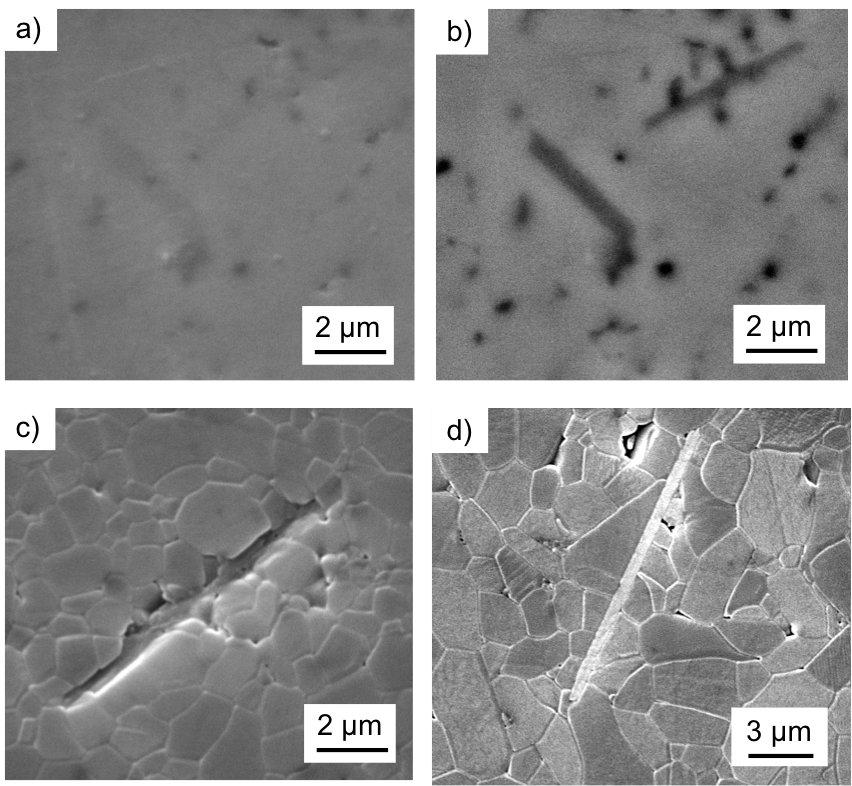
\includegraphics[width=\textwidth]{Chapter-5/Figures/Figure1.png}
	\caption{SEM micrographs of $\beta$-Al$_{2}$O$_{3}$ grains in a-c) Bayer alumina with 560 ppm Na$_{2}$O, 82 ppm SiO$_{2}$, and 380 ppm MgO after 3 h at 1525$^{\circ}$C and d) Bayer alumina with 29 ppm Na$_{2}$O, 103 ppm SiO$_{2}$, and 502 ppm MgO after 3 h at 1525$^{\circ}$C. The samples in a) and b) were not etched and the samples in c) and d) were etched. a), c), and d) were obtained using a secondary electron detector, and b) was obtained using a backscattered electron detector.}
	\label{Ch5-figure:Figure1}
\end{figure}
%%%

\newpage
%%%
\begin{figure}[H]
	\centering
	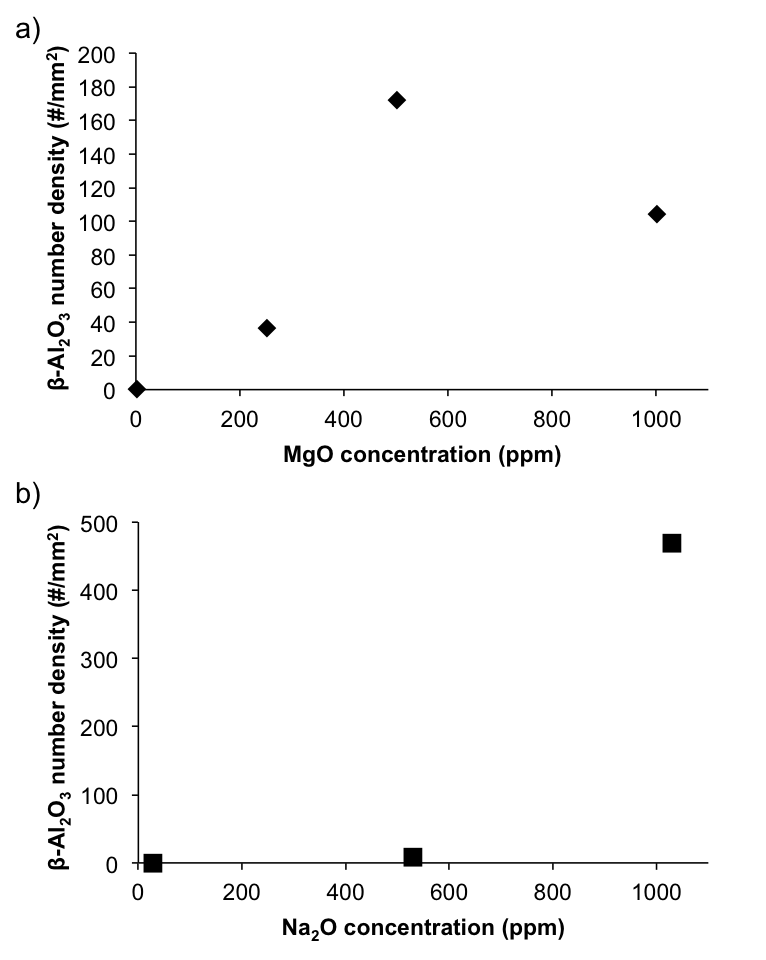
\includegraphics{Chapter-5/Figures/Figure2.png}
	\caption{Formation of $\beta$-Al$_{2}$O$_{3}$ in MgO-free powder samples as a function of a) MgO concentration and b) Na$_{2}$O concentration in samples after 3 h at 1525$^{\circ}$C.}
	\label{Ch5-figure:Figure2}
\end{figure}
%%%

\newpage
%%%
\begin{figure}[H]
	\centering
	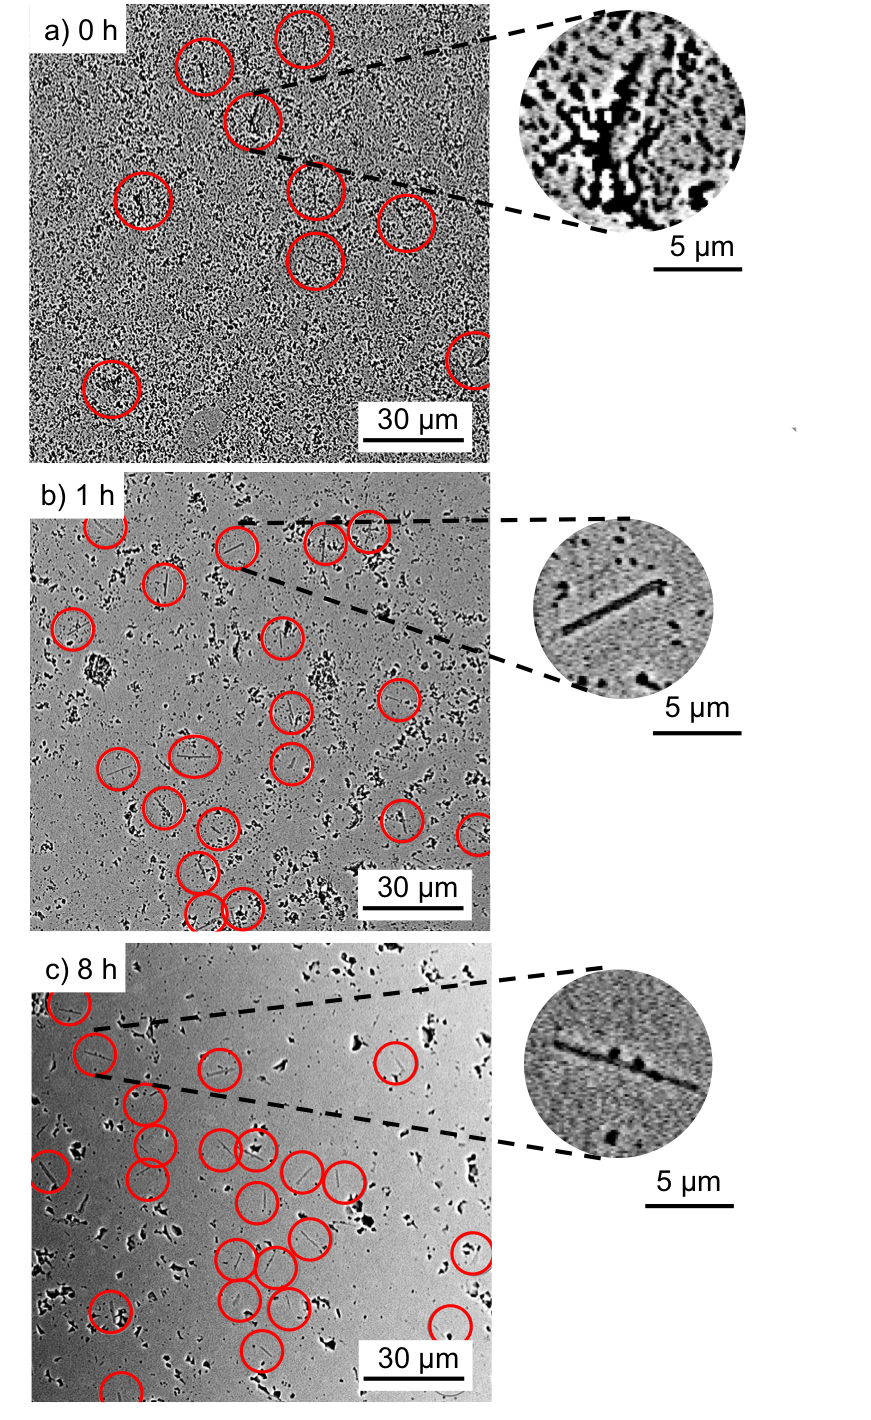
\includegraphics[scale=0.90]{Chapter-5/Figures/Figure3.png}
	\caption{Formation of $\beta$-Al$_{2}$O$_{3}$ a function of a) Na$_{2}$O concentration, b) SiO$_{2}$ concentration for different Na$_{2}$O concentrations, and c) of the Na$_{2}$O/SiO$_{2}$ ratio in MgO-doped (380 ppm) powder samples. In c) the black diamonds are samples with 82 ppm SiO$_{2}$ and the blue squares are samples with 182 and 582 ppm SiO$_{2}$.}
	\label{Ch5-figure:Figure3}
\end{figure}
%%%

\newpage
%%%
\begin{figure}[H]
	\centering
	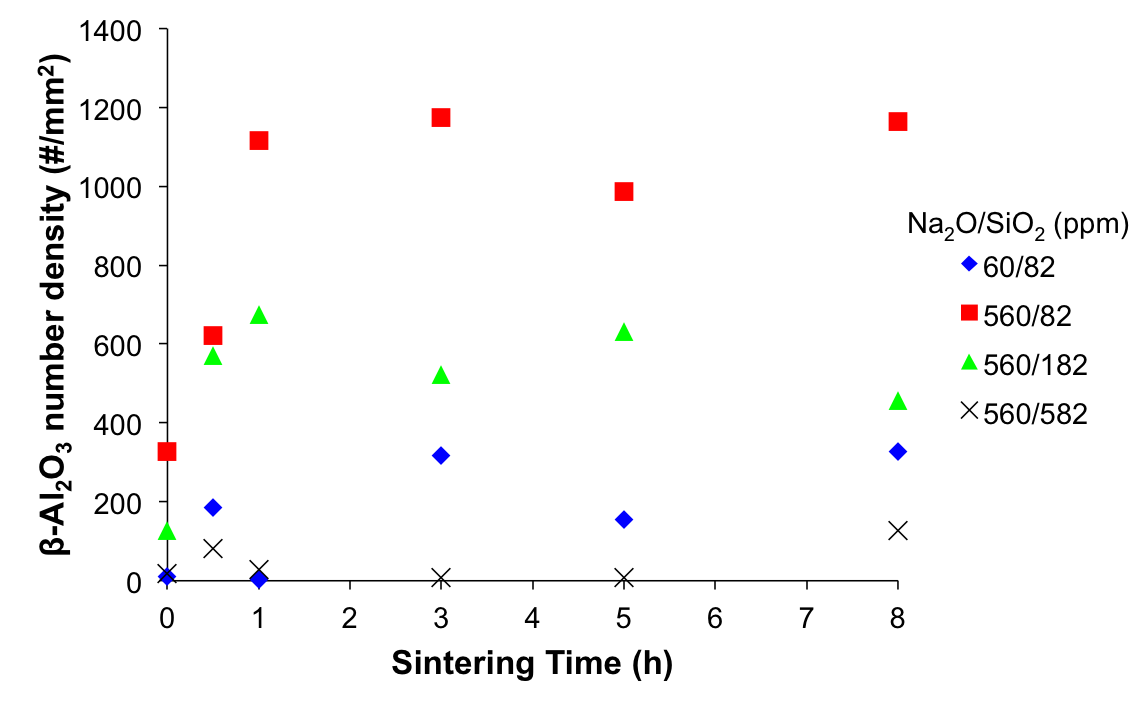
\includegraphics[width=\textwidth]{Chapter-5/Figures/Figure4.png}
	\caption{Kinetics of $\beta$-Al$_{2}$O$_{3}$ formation for different powder chemistries of MgO-doped powder samples (380 ppm MgO).}
	\label{Ch5-figure:Figure4}
\end{figure}
%%%

\newpage
%%%
\begin{figure}[H]
	\centering
	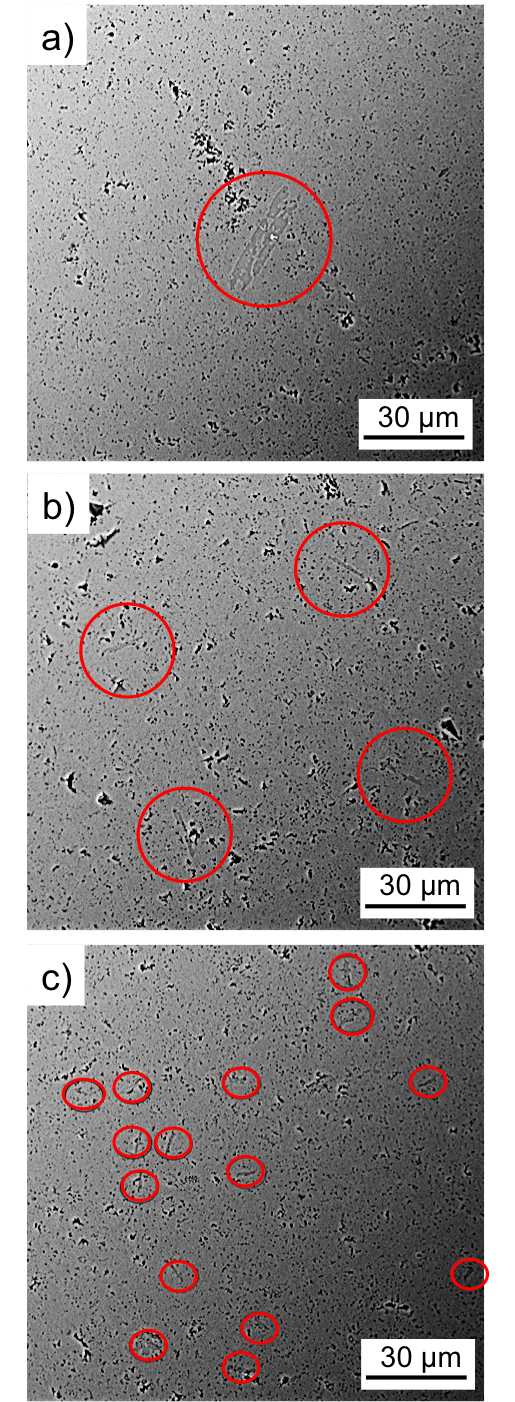
\includegraphics[scale=0.84]{Chapter-5/Figures/Figure5.png}
	\caption{Micrographs showing $\beta$-Al$_{2}$O$_{3}$ grains (red circles) in Bayer alumina samples with a) 1000 ppm MgO, 1000 ppm SiO$_{2}$, 29 ppm Na$_{2}$O, b) 2 ppm MgO, 1000 ppm SiO$_{2}$, 1000 ppm Na$_{2}$O, c) 1000 ppm MgO, 1000 ppm SiO$_{2}$, 1000 ppm Na$_{2}$O after 3 h at 1525$^{\circ}$C.}
	\label{Ch5-figure:Figure5}
\end{figure}
%%%

\newpage
%%%
\begin{figure}[H]
	\centering
	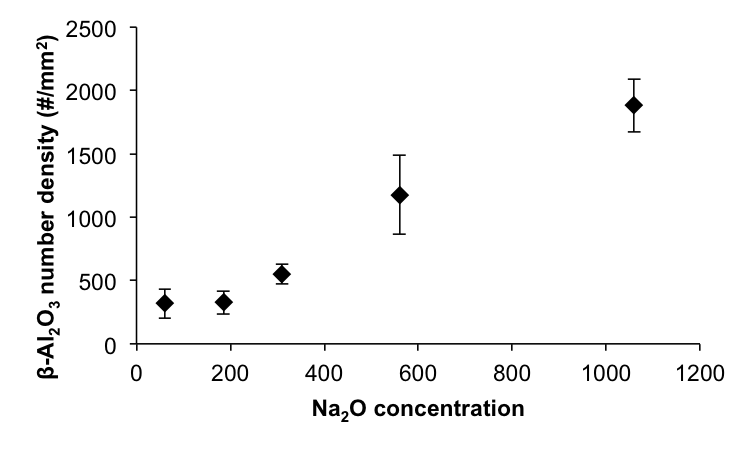
\includegraphics[scale=0.84]{Chapter-5/Figures/Figure6.png}
	\caption{Micrographs showing $\beta$-Al$_{2}$O$_{3}$ grains (red circles) in MgO-doped (380 ppm) Bayer alumina samples with 82 ppm SiO$_{2}$ and a) 185 ppm Na$_{2}$O, b) 560 ppm Na$_{2}$O, and c) 1060 ppm Na$_{2}$O after sintering at 1525$^{\circ}$C for 3 h.}
	\label{Ch5-figure:Figure6}
\end{figure}
%%%

\newpage
%%%
\begin{figure}[H]
	\centering
	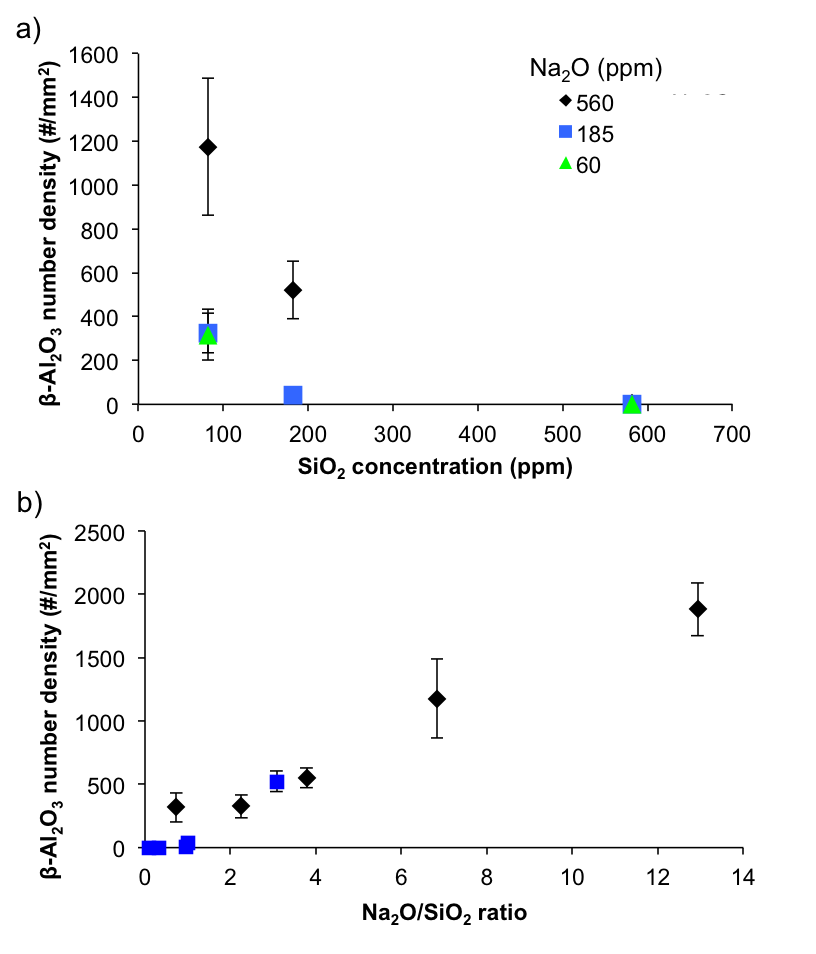
\includegraphics{Chapter-5/Figures/Figure7.png}
	\caption{Micrographs showing $\beta$-Al$_{2}$O$_{3}$ grains (red circles) in MgO-doped (380 ppm) Bayer alumina samples with a) 185/182 ppm Na$_{2}$O/SiO$_{2}$ and b) 560/182 ppm Na$_{2}$O/SiO$_{2}$ after sintering at 1525$^{\circ}$C for 3 h.}
	\label{Ch5-figure:Figure7}
\end{figure}
%%%

\newpage
%%%
\begin{figure}[H]
	\centering
	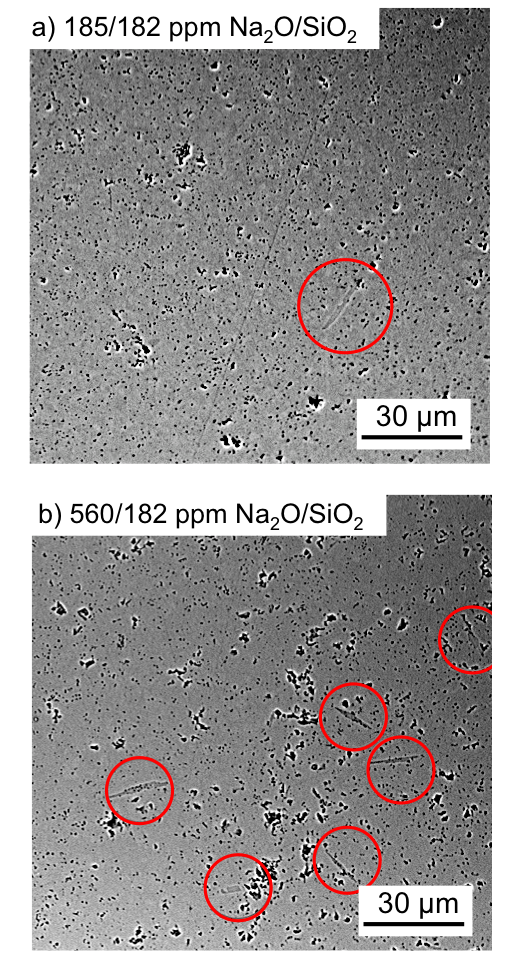
\includegraphics[scale=0.82]{Chapter-5/Figures/Figure8.png}
	\caption{Micrographs showing $\beta$-Al$_{2}$O$_{3}$ grains (red circles) in MgO-doped (380 ppm) Bayer alumina samples with 82 ppm SiO$_{2}$ and 560 ppm Na$_{2}$O after sintering at 1525$^{\circ}$C for a) 0 h, b) 1 h, and c) 8 h.}
	\label{Ch5-figure:Figure8}
\end{figure}
%%%

\newpage
%%%
\begin{figure}[H]
	\centering
	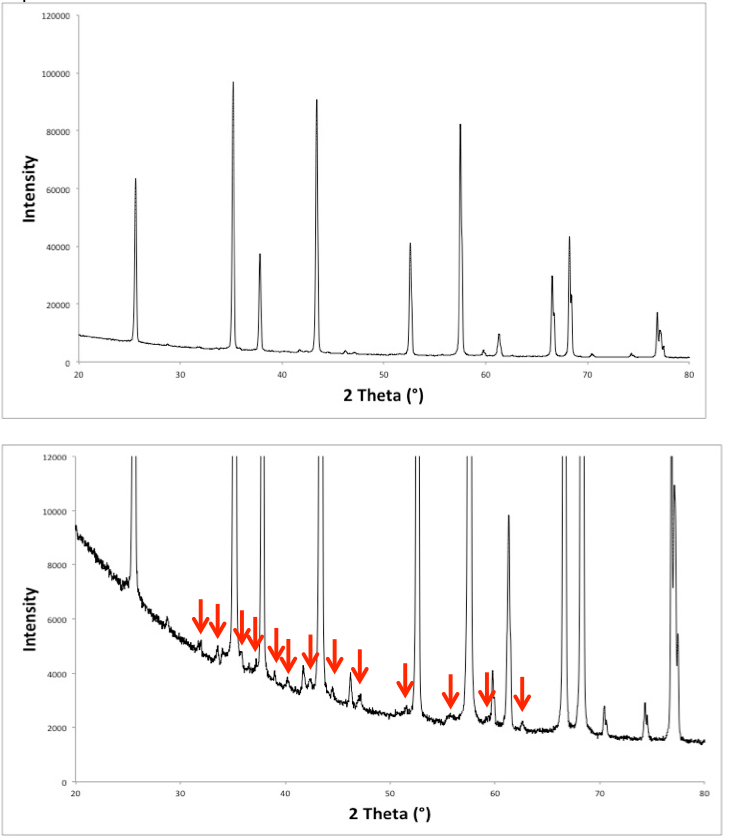
\includegraphics[width=\textwidth]{Chapter-5/Figures/Figure9.png}
	\caption{XRD pattern of a sample with 1060 ppm Na$_{2}$O, 82 ppm SiO$_{2}$, and 380 ppm MgO after sintering at 1525$^{\circ}$C for 5 h. The red arrows indicate the peaks that can be assigned to $\beta$-Al$_{2}$O$_{3}$. The other peaks can be assigned to $\alpha$-Al$_{2}$O$_{3}$.}
	\label{Ch5-figure:Figure9}
\end{figure}
%%%

\newpage
%%%
\begin{figure}[H]
	\centering
	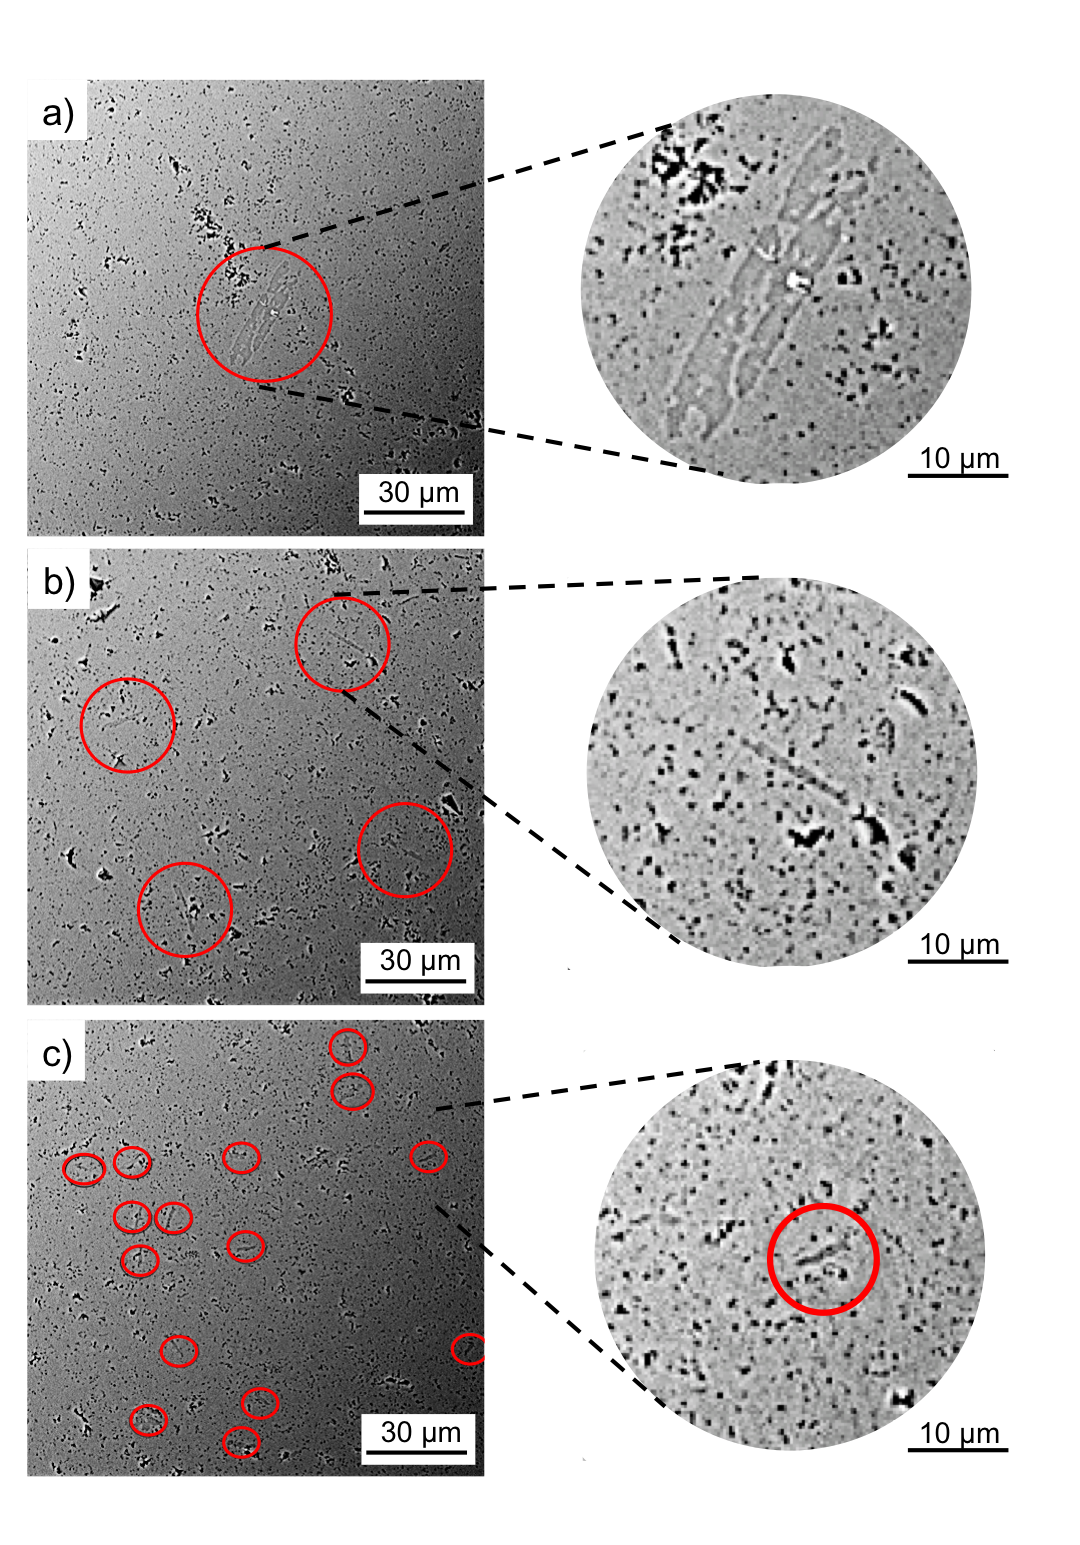
\includegraphics{Chapter-5/Figures/Figure10.png}
	\caption{Micrograph showing $\beta$-Al$_{2}$O$_{3}$ grains (red circles) in an ultra high purity powder sample with 502 ppm Na$_{2}$O, 2 ppm MgO, and 11 ppm SiO$_{2}$ after sintering at 1525$^{\circ}$C for 0 h.}
	\label{Ch5-figure:Figure10}
\end{figure}
%%%


\chapter{A Critique of the Master Sintering Curve Analysis of Sintering Processes}

\section{Introduction}
The master sintering curve (MSC) approach was developed by Su and Johnson\cite{Su1996a} to generalize the densification behavior of a sintering powder with a single curve for the entire sintering time/temperature profile. The MSC approach is based on a combined-stage sintering model developed by Hansen et al \cite{Hansen1992}, given as:

%%
\begin{equation}
\label{Ch6-eq: eq1}
\frac{1}{\rho} \frac{d\rho}{dt} = \frac{3 \gamma \Omega}{k_{B}T} \left( \frac{\delta D_{b} \Gamma_{b}}{G^{4}} + \frac{D_{v} \Gamma_{v}}{G^{3}} \right)
\end{equation}
%%

\noindent where $\rho$ is relative density of the powder compact, $d\rho/dt$ is densification rate, $\gamma$ is surface energy, $\Omega$ is molar volume, $k_{B}$ is Boltzmann's constant, $T$ is absolute temperature, $G$ is grain size, $D$ is diffusion coefficient, $\delta$ is grain boundary thickness, and $\Gamma$ is a geometric scaling factor. The subscripts $b$ and $v$ represent grain boundary and volume diffusion mechanisms, respectively. The MSC was originally derived to simplify the combined-stage sintering model (Eq. \ref{Ch6-eq: eq1}) to account for only a single diffusion mechanism, and by considering diffusion as thermally-activated with an activation energy $Q$. The resulting equation is given as:

%%
\begin{equation}
\label{Ch6-eq: eq2}
\frac{1}{\rho} \frac{d\rho}{dt} = \frac{3 \gamma \Omega}{k_{B}T} \left( \frac{D \Gamma}{G^{n}} \right)
\end{equation}
%%

\noindent where

%%
\begin{equation}
\label{Ch6-eq: eq3}
D = D_{0}e^{-Q/RT}
\end{equation}
%%

\noindent and $R$ is the ideal gas constant. Eq. \ref{Ch6-eq: eq2} is re-written to collect microstructural parameters on the left hand side and temperature dependent parameters on the right hand side:


%%
\begin{equation}
\label{Ch6-eq: eq4}
\frac{k_{B} G^{n}}{3 \rho \gamma \Omega \Gamma D_{0}} \frac{d\rho}{dt} = \frac{1}{T} exp \left( -\frac{Q}{RT} \right) = \frac{d \Theta}{dt}
\end{equation}
%%

\noindent Eq. \ref{Ch6-eq: eq4} can be integrated to give:

%%
\begin{equation}
\label{Ch6-eq: eq5}
\frac{k_{B} }{ \gamma \Omega \Gamma D_{0}} \int_{\rho_{0}}^{\rho} \frac{(G(\rho))^{n}}{3 \rho \Gamma (\rho)} d \rho = \int_{0}^{t} \frac{1}{T} exp \left( -\frac{Q}{RT} \right) dt = \Theta
\end{equation}
%%

\noindent Equation \ref{Ch6-eq: eq5} describes the sintering behavior for an arbitrary time-temperature profile, and the integral over this profile with respect to time is termed the work of sintering $\Theta$. The MSC is obtained by plotting $\rho$ versus $\Theta$. The left hand side of Eq. \ref{Ch6-eq: eq5} is not solved, because many of the parameters are unknown. However, as long as these parameters are independent of time and temperature, data plotted in this way will collapse into a single continuous curve for a single value of $Q$. It is interesting to note that the MSC analysis is independent of the sintering mechanism and, as a generalized model, was applied to other thermally activated process such as grain growth \cite{Park2006} and binder decomposition \cite{Diantonio2005,Aggarwal2007}.

In practice, $Q$ is a fitting parameter for which the best-fit MSC is obtained over a range of heating rates by determining the minimum mean residual. Assuming arbitrary values for $Q$ in Eq. \ref{Ch6-eq: eq5}, the mean residual square is calculated by \cite{Blaine2006}


%%
\begin{equation}
\label{Ch6-eq: eq6}
\mbox{Mean residual square} = \sqrt{\frac{1}{\rho_{s}-\rho_{0}}\int_{\rho_{0}}^{\rho_{s}} \frac{\Sigma_{i=1}^{N} \left( \frac{\Theta_{i}}{\Theta_{avg}}-1 \right)^{2}}{N} d\rho}
\end{equation}
%%

\noindent where $N$ is the number of experimental data points gathered at a series of heating rates and a sintered density $\rho_{s}$, and $Q_{avg}$ is the average of all $Q_{i}$ over $N$. The $Q$ value that yields the minimum mean residual square is the $Q$ value at which the MSC trajectories obtained from the densification curves at different heating rates yield the best fit and converge onto a single curve.  Because of the mechanistic nature of the model, the $Q$ parameter is usually referred to in the literature as the 'activation energy' for sintering.

MSC analysis has been applied to ceramic powders formed and densified by a variety of techniques. For high purity alumina, the reported $Q$ values vary drastically, as seen in Table \ref{Ch6-table:table1}. In Su and Johnson's original work \cite{Su1996a}, $Q$ values of 440 and 488 kJ/mol were determined by minimum mean residuals and iso-strain analysis, respectively, for an ultrafine, ultrahigh purity alumina (AKP-50, Sumitomo Chemical America, Inc.). These results showed that the activation energy obtained from minimum mean residuals is in close agreement with the activation energies determined by conventionally used methods. Using the same powder, Tatami et al. \cite{Tatami2006} determined a $Q$ of 555 kJ/mol, and when the powder was doped with 2000 ppm MgO, a $Q$ of 880 kJ/mol was determined. Pouchly et al. \cite{Pouchly2009} estimated the $Q$ of two different ultrahigh purity alumina powder graded (Taimicron TM-DAR, Taimei Chemicals and RC-HP DBM, Reynolds Chemicals) to be 770 and 640 kJ/mol, respectively, and attributed the difference in $Q$ to the difference in particle size of 110 nm and 240 nm, respectively. Aminzare et al. \cite{Aminzare2010}, reported $Q$ values of 700 and 605 kJ/mol for alumina (Taimicron TM-DAR, Taimai Chemicals) samples prepared by dry pressing and pressure filtration, respectively. Using the same alumina powder grade (Taimicron TM-DAR, Taimai Chemicals), Guillon and Langer \cite{Guillon2010} reported a $Q$ of 290 kJ/mol for Al$_{2}$O$_{3}$ densified by spark plasma sintering (SPS). They attributed the lower $Q$ value to the effect of the high heating rates of 35 - 150$^{\circ}$C/min during SPS. $Q$ values of up to 1064 kJ/mol were reported by Shao et al. \cite{Shao2009} for granulated and dry pressed alumina powder (350 nm, 99.9\%, Dalian Luming Nanometer Material Ltd.). They explained the higher $Q$ values as an effect of slower heating rates (0.5 and 5$^{\circ}$C/min) on densification.

The effect of heating rate on densification was explained by Harmer and Brook \cite{Harmer1981} as due to the relative time the material is heated under conditions favoring surface and grain boundary diffusion. They reasoned that a slow heating process favors surface diffusion and particle coarsening because surface diffusion usually has a lower activation energy than densification mechanisms such as grain and volume diffusion. Samples heated at slow rates spend relatively longer times at lower temperatures and, therefore, experience more particle coarsening prior to reaching the temperatures where densification occurs. Thus, the sintering driving force provided by surface area is higher during the densification stage when ceramics are fired at higher heating rates since these samples do not undergo as much coarsening prior to densification. In MSC analysis, these relative changes in mechanism result in lower $Q$ values at faster heating rates. However, it is assumed in the MSC analysis that sintering occurs by a single mechanism for the heating conditions used to collect densification data. Since data for MSC analysis is performed by heating samples at different heating rates, the contributions from surface diffusion and grain boundary diffusion vary, and it is questionable if the $Q$ values obtained can be used for mechanistic interpretations. Furthermore, it is not apparent what other parameters, additionally to the heating rate, cause the large variability of the reported $Q$ values.  

In this work we investigate how forming techniques and powder chemistry affect the $Q$ parameter and the shape of the MSC for a commercial specialty alumina powder. We explore how forming process-induced differences in relative green density, microstructural homogeneity and shrinkage anisotropy affect the value of $Q$. We also investigate how the assumption of a constant microstructure (i.e., grain size) at high density affects the MSC fit and $Q$ value. A series of Na$_{2}$O-doped samples were studied to determine how changes in densification mechanism affect the value of $Q$.  Based on these experiments, we discuss the limits and accuracy of the MSC approach and then determine how MSC can be used in a constructive, practical way to predict the sintering of a specific powder.

\section{Experimental Procedure}

To examine the impact of the forming technique on the MSC, we prepared undoped alumina (CT3000 LS SG, Almatis, Inc., Leetsdale, PA) samples by dry pressing, slip casting and tape casting. The powder was a specialty reactive alumina (99.8\%) with an average particle diameter of $\sim$0.3 $\mu$m. Two sets of samples were prepared by uniaxial dry pressing. For one set, the as-received powder was sieved to -106 $\mu$m and uniaxially dry pressed at 30 MPa. The powder handling for the second set was designed to produce a soft granule powder by dispersing it in ethanol with 5 wt.\% polyethylene glycol (PEG 600, Alfa Aesar, Ward Hill, MA, USA). After ball milling for 24 h, the dried powder was sieved to -106 $\mu$m and samples were lightly pressed at 30 MPa. For uniaxial dry pressing a bar shaped die was used, where the long axis was perpendicular to the pressing direction to minimize density gradients. Both sample types were iso-pressed at 200 MPa after removing the organic processing aids by heating at 600$^{\circ}$C for 12 h in air.

For tape casting, a slurry was prepared by ball milling 26 vol.\% alumina powder with 29.7 vol.\% xylene (ACS Reagent grade, Avantor Performance Materials, Inc., Center Valley, PA, USA), 32.3 vol.\% ethanol (200 proof), and 2.1 vol.\% blown menhaden fish oil (Grade Z-3, Tape Casting Warehouse, Morrisville, PA, USA). After 24 h, 5.2 vol.\% polyvinyl butyral (PVB B-98, Tape Casting Warehouse, Morrisville, PA, USA), 2.3 vol.\% polyalkylene glycol (PAG, UCON50HB2000, Tape Casting Warehouse, Morrisville, PA, USA) and 2.5 vol.\% butyl benzyl phthalate (BBP S-160, Tape Casting Warehouse, Morrisville, PA, USA) were added and the mixture was ball milled for another 24 h. Subsequently 1 drop of cyclohexane (99$+$\%, Alfa Aesar, Ward Hill, MA, USA) per 20 g of alumina powder was added and the slurry was stirred for an additional 45 min. The slurry was tape cast on a silicone-coated Mylar$^{TM}$ carrier tape using a doctor blade gap height of 305 $\mu$m. After drying, the tape was cut, stacked, uniaxially pressed at 70$^{\circ}$C for 10 min at minimal pressure to tack the layers together, and then isostatically laminated at 74$^{\circ}$C and 20 MPa for 30 min.

For non-aqueous slip casting, 28.9 vol.\% powder was dispersed in xylene with 3.8 vol.\% Menhaden fish oil, ball milled for 24 h, and slip cast. For aqueous slip casting 44.6 vol.\% alumina powder was dispersed in deionized water with 6.3 vol.\% Darvan C (R. T. Vanderbilt Company, Inc., Norwalk, CT, USA). The pH of the Darvan and water mixture was adjusted to 11 using 5 M NH$_{4}$OH before the alumina powder was added. The slurry was ball milled for 24 h and then slip cast. In both cases the mold consisted of a PVC tube (20 mm diameter) on a plaster of Paris plate.

The polymer processing aids were burned out of all samples by heating at 600$^{\circ}$C for 12 h in air. All samples were cold isostatically pressed at 200 MPa (CIP, Autoclave Engineers, Erie, PA). The samples were subsequently cut and ground into 3 x 3 x 15 mm$^{3}$ bars for dilatometry studies. The long axis of the dilatometry samples is perpendicular to the casting direction during slip casting and parallel to the casting direction for tape cast samples. The bars were heated to 1525$^{\circ}$C or 1595$^{\circ}$C at 5, 10, and 20$^{\circ}$C/min in a thermomechanical analyzer (TMA; Linseis PT1600, Robbinsville, NJ) and held at temperature for 5 min to record the linear shrinkage of the samples. The thermal expansion of the test fixture was removed by blank experiments, and the thermal expansion contribution of the samples to the dilatometry curves was subtracted from the dimensions measured in-situ using the cooling curves of the samples measured in the TMA. To ensure accurate shrinkage values the initial nonzero value of the dilatometry data was eliminated, as described in the literature \cite{Blaine2006}.

To examine how changes in chemistry affect the MSC analysis, we studied a series of non-aqueous slip cast Na$_{2}$O-doped aluminas. The alumina powder was doped with up to 1000 ppm Na$_{2}$O using sodium acetate (NaC$_{2}$H$_{3}$O$_{2}$*3H$_{2}$O, ACS grade, BDH, West Chester, PA). The detailed doping procedure is reported in chapter 2.


\section{Results and Discussion}

\subsection{The effect of forming on $Q$}

During initial studies, we observed different degrees of anisotropic shrinkage as a function of the forming method. For example, the dilatometry curves of the non-aqueous slip cast samples during heating to 1525$^{\circ}$C at 5, 10, and 20$^{\circ}$C/min are shown in Figure 1\ref{Ch6-figure:Figure1}. The shrinkage was measured in the z-direction, i.e., the direction parallel to the capillary (i.e. shear) force of the plaster of Paris mold during slip casting, and in the x/y-direction, perpendicular to the capillary force. Anisotropic shrinkage was observed for all heating rates. Samples heated at 5$^{\circ}$C/min have a higher shrinkage in the z-direction than in the x/y-direction throughout the entire sintering process, whereas samples heated at 10 and 20$^{\circ}$C/min show slightly more shrinkage in the x/y-direction in the initial stage of densification followed by a crossover in the shrinkage and much more shrinkage in the z-direction at higher densities. The anisotropic shrinkage was quantified with a shrinkage anisotropy factor $k$, which is the ratio of the shrinkage in x/y-direction to the shrinkage in z-direction. Figure \ref{Ch6-figure:Figure2} shows how $k$ changes as a function of relative density and heating rate for the non-aqueous slip cast samples heated at different heating rates during densification. Interestingly, the shrinkage anisotropy factor changes significantly as a function of heating rate during densification and there is much less change in $k$ at the slowest heating rate. Relative density was calculated using the shrinkage anisotropy factor and is plotted as a function of temperature in Figure \ref{Ch6-figure:Figure3}. The mean residuals were calculated as a function of $Q$ (Eq. \ref{Ch6-eq: eq6}), and the minimum is at $Q$ = 550 kJ/mol (Figure \ref{Ch6-figure:Figure4}). The relatively sharp minimum provides evidence that a single MSC curve is a good fit for the measured TMA data. 

When shrinkage in the z-direction is assumed to represent isotropic shrinkage (i.e. $k$=1), then $Q$ increases to 625 kJ/mol. Figure \ref{Ch6-figure:Figure5} compares the MSCs obtained when the shrinkage anisotropy was accounted for (550 kJ/mol) or by assuming isotropic shrinkage (no correction for anisotropy). This example demonstrates the importance of determining whether the sample shrinks anisotropically during the density measurements used to construct the MSC, and the need to correct for anisotropic shrinkage to determine an accurate value $Q$ and MSC. Note that the curves at all three heating rates coincide.

Figure \ref{Ch6-figure:Figure6} shows the corresponding MSC curves of samples formed by various techniques and heated to 1525$^{\circ}$C. The measurements were corrected for shrinkage anisotropy as described above. The total shrinkage anisotropy was $\sim$0.75 for slip cast and tape cast samples, and $\sim$0.92 for dry pressed samples. It is clear that $Q$ changes as a function of forming technique, which is, in part, due to different green densities. The sample prepared by non-aqueous slip casting has a green density of 59\% and the lowest $Q$ (550 kJ/mol), followed by the sample prepared by aqueous slip casting with a green density of 58\% and a $Q$ of 650 kJ/mol. The samples prepared by dry pressing (no PEG) and tape casting have green densities of 57\% and 55\%, respectively, and both samples have a $Q$ of 730 kJ/mol. The dry pressed sample with 5 wt.\% PEG has a green density of 55\% and the highest activation energy with 810 kJ/mol. It can thus be observed that $Q$ decreases as the green density increases and that the shape and position of the MSC changes as a function of forming technique (Figure \ref{Ch6-figure:Figure6}). Aminzare et al. \cite{Aminzare2010} also observed that $Q$ is sensitive to the forming technique and concluded that samples prepared by pressure filtration have a lower $Q$ than dry pressed samples as a result of better sample homogeneity as evidenced by the higher green density. As shown in this work, the effect of green density on $Q$ is complicated. For example, the samples prepared by tape casting and dry pressing with 5 wt.\% PEG have the same green density of 55\%, but different $Q$ values of 730 kJ/mol and 810 kJ/mol, respectively, and different MSC shapes. This suggests that other sample characteristics, in addition to green density, influence $Q$, such as pore size, pore size distribution, and particle/pore orientation. Given that the curves shown in Figure \ref{Ch6-figure:Figure6} diverge at very low density it can be assumed that additional factors, i.e. factors that are assumed to be constant in MSC analysis such as $D_{0}$, are highly variable and depend strongly on process history. The magnitude of differences observed suggest that these variables are extremely important in understanding differences in sintering behavior. Such changes are not related to activation energy and have been largely overlooked or ignored in prior literature.

\subsection{MSC at high densities}
The final densities used in the MSC analysis of the samples discussed above are $\leq$90\%. Above 90\% density we observed that the MSC curves for different heating rates diverge and thus dramatically influences the value of $Q$. Figure \ref{Ch6-figure:Figure7}a shows the densification curves of dry pressed samples sintered to >95\% density when heated to 1595$^{\circ}$C at different heating rates and held for 5 min. The minimum mean residual analysis yielded $Q$ = 700 kJ/mol (Figure \ref{Ch6-figure:Figure7}b) and Figure \ref{Ch6-figure:Figure7}c shows the resulting MSC. It can be seen that $Q$ = 700 kJ/mol gives a good fit at low densities, but the trajectories begin to diverge at densities >90\% (see Fig \ref{Ch6-figure:Figure7}c insert). 

To account for the effect of bulk density on densification we determined the activation energy at some relative densities by plotting $ln(-T \cdot d\rho/dt)$ vs. $1/T$ and determining the slopes of the resulting linear curves of the isodensities. Figure \ref{Ch6-figure:Figure8} shows the development of the apparent activation energy obtained from iso-density analysis, $Q_{iso}$, and it can be seen that $Q_{iso}$ is $\sim$700 kJ/mol and increases slightly with increasing relative density. At densities >85\% $Q_{iso}$ increases somewhat more rapidly, and at densities >95\% $Q_{iso}$ increases drastically to >1800 kJ/mol. This change in $Q_{iso}$ explains the divergence of the MSC trajectories obtained from the different heating rates using $Q_{MSC}$ = 700 kJ/mol. 

At densities <90\% the activation energy obtained from the minimum mean residuals $Q_{MSC}$, which is used to obtain the MSC, is reasonably close to the activation energies obtained from the iso-density analysis, $Q_{iso}$, resulting in a good fit at all heating rates. However, at densities >90\% where we observe divergence in the MSCs, the values of $Q_{iso}$ are >100 kJ/mol greater than the $Q_{MSC}$ value used to construct the MSC. Although the idea of variable activation energy is understandable, it is not physically realistic to consider that the activation energy for sintering is intrinsically a function of $\rho$. It is more likely that this increase in $Q_{iso}$ and the divergence of the MSC at high densities is caused by microstructural or mechanistic changes that are not accounted for in the MSC model. 

\subsection{Quantification of the MSC shape}
A way to account for microstructural changes is analyzing the shape of the MSC, since it is determined by the evolution of the microstructural parameters in the left hand side of Eq. 5. Microstructural evolution can be described quantitatively by:

%%
\begin{equation}
\label{Ch6-eq: eq7}
C = \frac{k_{B} G^{n}}{3 \gamma \Omega \Gamma D_{0}}
\end{equation}
%%

\noindent By rearranging Eq. \ref{Ch6-eq: eq4}, $C$ can be determined as a function of relative density:

%%
\begin{equation}
\label{Ch6-eq: eq8}
C = \rho \frac{d \Theta}{d \rho}
\end{equation}
%%

\noindent In Figure \ref{Ch6-figure:Figure9} it can be seen that $C$ increases by more than 5 orders of magnitude between 57\% and 98\% relative density. The increase in $C$ is partially due to the 8-fold increase in grain size from 0.3 to 2.4 $\mu$m during sintering of the sample to 98\% relative density. Assuming that grain boundary diffusion controls densification ($n$=4), the coarsening of the microstructures accounts for an increase in $C$ of $\sim$3.5 orders of magnitude. The remaining $\sim$2 orders of magnitude increase in $C$ are most likely due to an increase in the geometric factor $\Gamma$, since it is a function of relative density and the only parameter that is expected to change considerably with temperature. Note that the obtained trajectories for $C$ also diverge above 90\% relative density, similar to the MSCs.

While we can hypothesize about the factors that influence the MSC shape, the actual shape of the MSC cannot be understood based on the existing MSC analysis methodology, because one or more parameters in Eq. \ref{Ch6-eq: eq7} vary with time and temperature in a complex manner. To gain insight into the development of the shape of the MSC the individual parameters in Eq. \ref{Ch6-eq: eq7} need to be investigated. For example, grain size evolution could be tracked as a function of density and extracted from the $C$ parameter. Assuming that the divergence of the MSCs at densities >90\% is caused by differences in grain size as a result of different heating rates only, this divergence in MSC shape at densities >90\% could be corrected. If the development of the geometry factor $\Gamma$ could be quantified and separated from the $C$ parameter, we should be able to assign a constant value for $C$, and the $Q$ value that results from MSC analysis should represent the true activation energy for sintering. However, such an analysis would assume that $\Gamma$ can be quantified on a sufficiently accurate level, and that grain size and $\Gamma$ are the only factors in Eq. \ref{Ch6-eq: eq7} that change as a function of relative density.

\subsection{Influence of powder chemistry}

Figure \ref{Ch6-figure:Figure10} shows the MSCs of Na$_{2}$O-doped samples formed by non-aqueous slip casting. It can be seen that $Q$ changes as a function of Na$_{2}$O concentration and increases from 550 kJ/mol for samples with no Na$_{2}$O dopant to 700 and 730 kJ/mol for samples doped with 250 and 500 ppm Na$_{2}$O, respectively. $Q$ decreases to 690 kJ/mol when the concentration is further increased to 1000 ppm Na$_{2}$O. The position of the MSC changes as a function of Na$_{2}$O concentration as well and the effect of Na$_{2}$O concentration on the MSC is complicated.

\subsection{Limitations of the MSC analysis}

Anisotropic shrinkage is commonly observed in slip cast parts since the capillary force cause particles in the slurry to align during slip casting. It should be noted that the degree of shrinkage anisotropy strongly depends on the particle morphology and forming technique (i.e. magnitude of shear force exerted on the particles and ease of reorientation). For samples that were prepared by colloidal forming techniques, such as slip casting and tape casting, the degree anisotropic shrinkage has to be taken into account during the MSC analysis, otherwise the densities calculated from the dilatometry data alone are inaccurate and thus the calculated value of $Q$ and the shape of the MSC are incorrect. Likewise, samples formed by uniaxial pressing are often anisotropic but not to the same degree as slurry processed ceramics.

The above results show that a variety of factors such as forming technique and powder chemistry affect the value of $Q$ and the shape of the MSC in a complicated way, and the reason for this complicated relation lies in the assumption in MSC analysis that sintering is influenced by only one single mechanism. Making this assumption allows MSC analysis to assign an activation energy for sintering that corresponds to this specific sintering mechanism. If this assumption held true, variations in forming technique or chemistry could be analyzed using the MSC approach and using $Q$ as an indicator for how the sinterability of a powder changes as a function of powder chemistry and forming technique. However, sintering is typically divided into different stages, all of which are governed by different sintering mechanisms. When multiple mechanisms are involved, each mechanism can be affected differently by such changes and $Q$ loses its physical meaning as an activation energy for a specific sintering mechanism. As a result, $Q$ appears to be a function of relative density (Figure \ref{Ch6-figure:Figure8}) and the changes in $Q$ and MSC shape as a function of powder chemistry and forming technique are complicated (Figures \ref{Ch6-figure:Figure9} and \ref{Ch6-figure:Figure10}). 

For example, we know that initial pore size, pore size distribution, \newline and pore/particle orientation in a green body are highly dependent on the forming technique. Changes in these parameters affect different sintering stages in different ways. During initial stage sintering the sinter undergoes a particle rearrangement process that is driven by capillary forces and therefore highly sensitive to the aforementioned parameters. During final stage sintering the concentration of large pores that can only slowly be eliminated is determined by the forming technique. Mechanistic changes as such can affect $Q$ in different ways.

Similarly, powder chemistry affects initial stage sintering and intermediate stage sintering in different ways. In previous chapters, it was observed that the onset temperature of sintering increases with higher Na$_{2}$O concentration, which has the effect of increasing $Q$. The further development of densification was shown to depend heavily on additional factors. For example, samples with Na$_{2}$O/SiO$_{2}$ ratios $\sim$1.0 densify faster during intermediate stage sintering than samples with Na$_{2}$O/SiO$_{2}$ ratios $\sim$0.1 for the same SiO$_{2}$ concentration because Na$_{2}$O decreases the viscosity of the siliceous liquid grain boundary phase, and, therefore, enhances diffusion, which would decrease $Q$. This demonstrates that powder chemistry influences fundamental sintering mechanisms at different sintering stages and in different ways. 

Since the processes and mechanisms of all sintering stages are lumped into one $Q$ value during MSC analysis, forming technique and powder chemistry may affect the value of $Q$ and the shape of the MSC, but the changes in sintering behavior and mechanisms cannot be sufficiently described using $Q$ and the MSC. Therefore, the MSC approach is judged to be insufficient to evaluate forming and powder chemistry effects on sintering. It is recommended that $Q$ values obtained by MSC analysis for different powder grades (i.e. chemistries, forming techniques, particle size, etc.) should not be compared or used to draw conclusions about sintering mechanisms.

\subsection{Practical use of the MSC analysis}

Even though MSC analysis is insufficient to analyze fundamental differences in sintering behavior due to differences in powder chemistry and forming technique, choosing an appropriate $Q$ value converges the trajectories of samples obtained from different heating rates onto one MSC, and this $Q$ value and the obtained MSC can be used to predict densification. As explained in the literature \cite{Wang2010,Reiterer2009}, the $Q$ value obtained is an apparent activation energy for the entire sintering process of a sinter and accounts for densification (regardless of mechanism), the retardation of densification due to grain growth, surface diffusion in the early sintering stages, and other processes that potentially influence densification. Consequently, $Q$ is a fitting parameter that is composed of a variety of factors that influence densification, including the activation energies for sintering of all involved mechanisms. 

One of the practical objectives of MSC analysis is to predict the sintered density of samples prepared from a given powder for an arbitrary time/temperature condition. The MSC data provided above and Eq. \ref{Ch6-eq: eq5} can be used to construct equivalent time/temperature diagrams to predict the density of samples for known heating conditions \cite{Aminzare2010}. Fig. \ref{Ch6-figure:Figure11} is an example of the equivalent time/temperature conditions leading to equivalent densities for non-aqueous processed powder dry pressed samples heated at 10$^{\circ}$C/min. The contours shown in Figure \ref{Ch6-figure:Figure11} indicate the equivalent relationships between particular time/temperature treatments and relative densities of 80, 85, 90, and 95\%. For example, a relative density of 85\% is reached after heating a dry pressed sample at 10$^{\circ}$C/min to 1460$^{\circ}$C with no hold time. The same density is reached after heating a dry pressed sample from the same powder at 10$^{\circ}$C/min to 1400$^{\circ}$C and holding for 29 min. It should be noted that the predicted MSC response for >90\% sintered density has some inaccuracy due to the discrepancies we noted above for MSC data analysis at >90\% density. Despite earlier reservations and limitations, the predictions for equivalent time/temperature conditions leading to 95\% density are insightful and, at least, give a semiquantitative measure of the effect of time and temperature on sintering. In the literature it was proposed to divide the MSC into two regimes of "low density" and "high density" (i.e., <75\% and >85\%), respectively with two individual $Q$ values to account for the changes in $Q$ during densification \cite{Pouchly2009,Maca2014}. While the fundamental reasoning behind assigning two separate $Q$ values is questionable, considering our conclusion that $Q$ is a fitting parameter without physical meaning, this could be an useful approach to obtain more accurate density predictions at high densities.

\section{Summary}
MSC analysis results in two pieces of information; a $Q$ value and the MSC curve itself. $Q$ should not be interpreted as the activation energy for sintering, since multiple mechanisms contribute to its value and processing history and powder chemistry can drastically affect the $Q$ value and the shape of the MSC. Therefore, comparing $Q$ between different chemistries is not an appropriate means to interpret fundamental, mechanistic changes in sintering behavior. 

It is evident that the MSC is only useful for characterizing the sintering behavior of the specific ceramic powder studied. A number of factors need to be accounted for to obtain accurate $Q$ values and MSCs including sample shrinkage anisotropy, and limiting the density range to < 90\% density to avoid microstructural changes that are not accounted for in the MSC analysis. With more accurate $Q$ values the MSC approach is a useful tool and "a practical approach to sintering" as originally proposed by Su and Johnson, but is not sufficient to explain fundamental changes in sintering behavior, or to determine the "activation energy" for sintering since basic assumptions made for MSC analysis are insufficient to describe the entire sintering process.

\newpage
\begin{table}[H]
	\caption{$Q$ values obtained by MSC analysis for different alumina powders.}
	\centering
	\begin{tabular}{ | c | c | c | c | c | }
		\hline
		Alumina grade & Forming technique & Heat rates & $Q$ & Ref.\\
		& & ($^{\circ}$C/min) & (kJ/mol) & \\
		\hline
		AKP-50 & CIP (270 MPa) & 60 to & 440 & \cite{Su1996a}\\
		Sumitomo & & 750$^{\circ}$C, & & \\
		Chemicals & & 8-45 to & & \\ 
		& & 1500$^{\circ}$C & & \\
		\hline
		AKP-50 & Uniaxial pressing & 3-20 to & 555 & \cite{Tatami2006} \\
		Sumitomo & (50 MPa) & 1400$^{\circ}$C & & \\
		Chemicals & CIP (200 MPa) & & & \\
		\hline
		AKP-50 +  & Uniaxial pressing (50 MPa) & 3-20 to & 880 & \cite{Tatami2006} \\
		2000 ppm MgO & CIP (200 MPa) & 1400$^{\circ}$C & & \\
		Sumitomo Chemicals & & & & \\
		\hline
		Taimicron TM-DAR & CIP (300 MPa) & 2-20 to & 770 & \cite{Pouchly2009}\\
		Taimei Chemicals & & 1500$^{\circ}$C & & \\
		\hline
		RC-HP DBM & CIP (300 MPa) & 2-20 to & 640 & \cite{Pouchly2009}\\
		Reynolds Chemicals & & 1500$^{\circ}$C & & \\
		\hline
		Taimicron TM-DAR & Uniaxial pressing (50 MPa) & 2-25 to & 700 & \cite{Aminzare2010}\\
		Taimei Chemicals & CIP (200 MPa) & 1400$^{\circ}$C & & \\
		\hline
		Taimicron TM-DAR & Pressure filtration & 2-25 to & 605 & \cite{Aminzare2010}\\
		Taimei Chemicals & (40 MPa) & 1400$^{\circ}$C & & \\
		\hline
		Taimicron TM-DAR & SPS (50 MPa) & 35-150 to & 290 & \cite{Guillon2010}\\
		Taimei Chemicals & & 1200$^{\circ}$C & & \\
		\hline
		99.9\%, & Uniaxial pressing & 0.5-5 to & 1064 & \cite{Shao2009}\\
		Dalian Luming & (80 MPa) & 1640$^{\circ}$C & & \\
		Nanometer Materials & CIP (250 MPa) & & & \\
		\hline
	\end{tabular}
	\label{Ch6-table:table1}
\end{table}
%%%

\newpage
%%%
\begin{figure}[H]
	\centering
	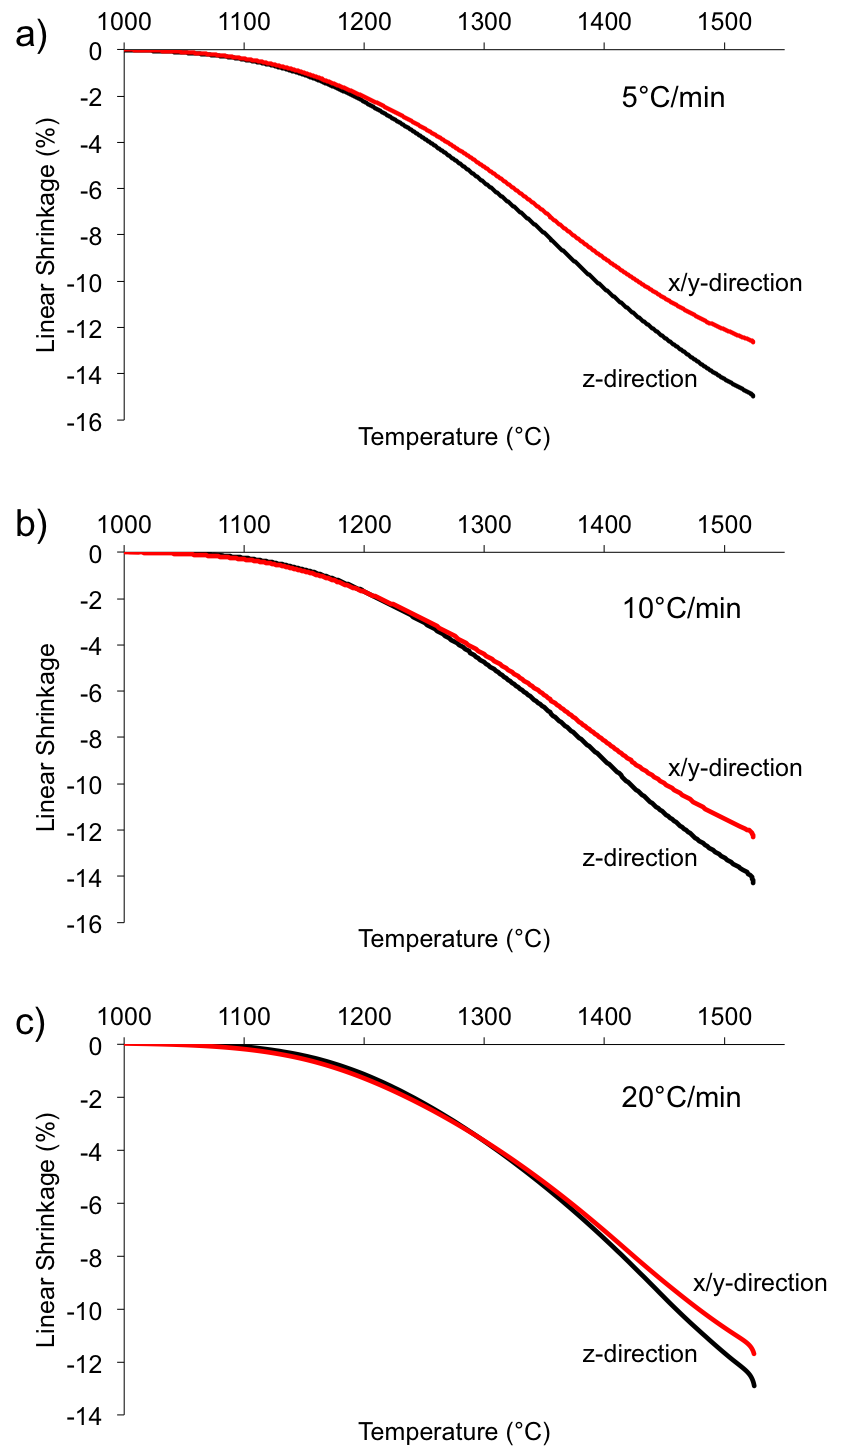
\includegraphics[scale=0.80]{Chapter-6/Figures/Figure1.png}
	\caption{Dilatometry curves of non-aqueous slip cast CT3000 LS SG samples heated at a) 5$^{\circ}$C/min, b) 10$^{\circ}$C/min, and c) 20$^{\circ}$C/min to 1525$^{\circ}$C measured parallel to (z-direction) and perpendicular to (x/y-direction) the capillary force acting during slip casting.}
	\label{Ch6-figure:Figure1}
\end{figure}
%%%

\newpage
%%%
\begin{figure}[H]
	\centering
	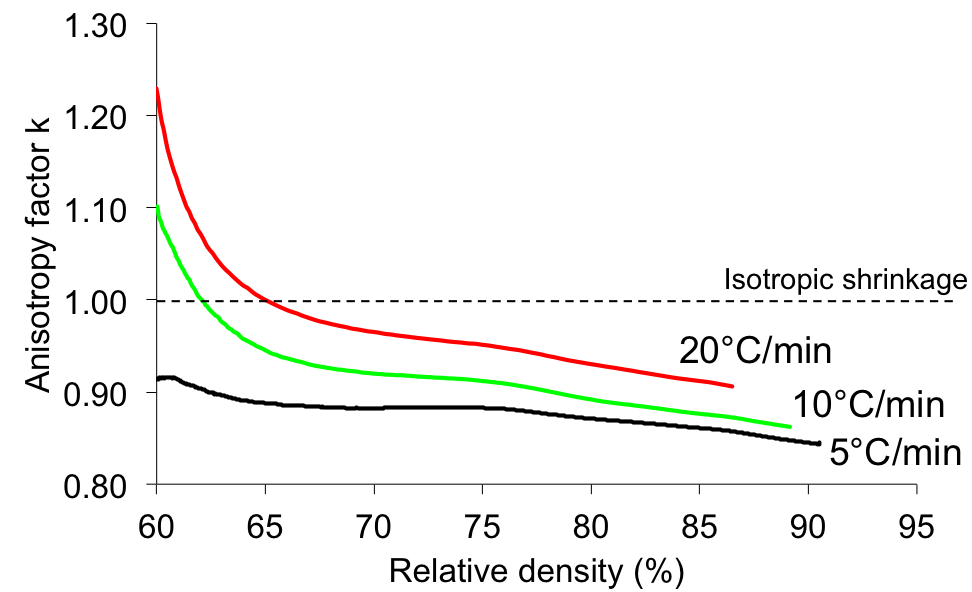
\includegraphics[width=\textwidth]{Chapter-6/Figures/Figure2.png}
	\caption{Development of the shrinkage anisotropy factor for shrinkage, $k$, during densification of non-aqueous slip cast samples as a function of relative density for CT3000 LS SG samples heated at different rates.}
	\label{Ch6-figure:Figure2}
\end{figure}
%%%

\newpage
%%%
\begin{figure}[H]
	\centering
	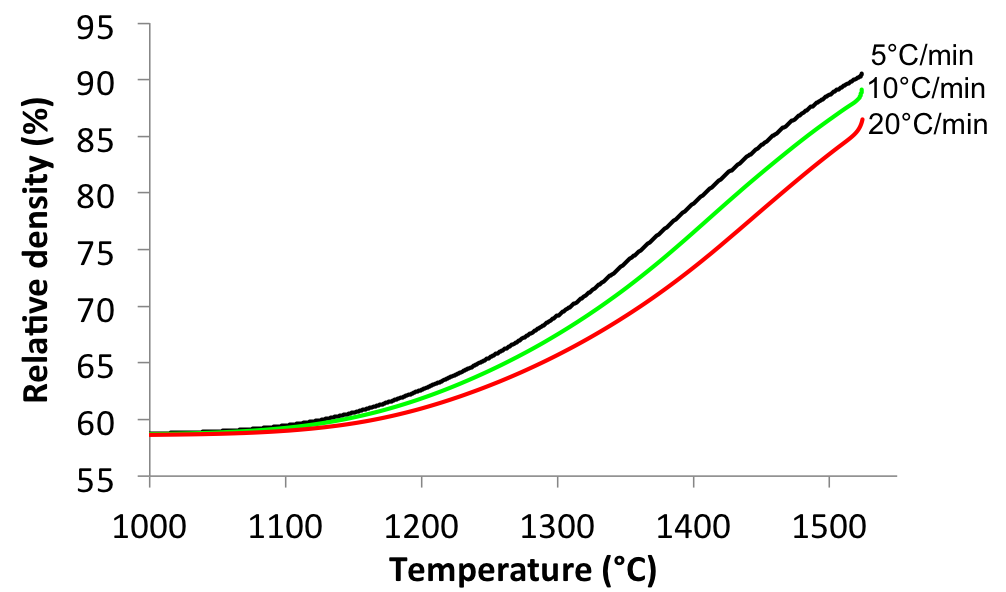
\includegraphics[width=\textwidth]{Chapter-6/Figures/Figure3.png}
	\caption{Development of the relative density corrected for shrinkage anisotropy as a function of temperature for non-aqueous slip cast CT3000 LS SG samples heated at different rates.}
	\label{Ch6-figure:Figure3}
\end{figure}
%%%

\newpage
%%%
\begin{figure}[H]
	\centering
	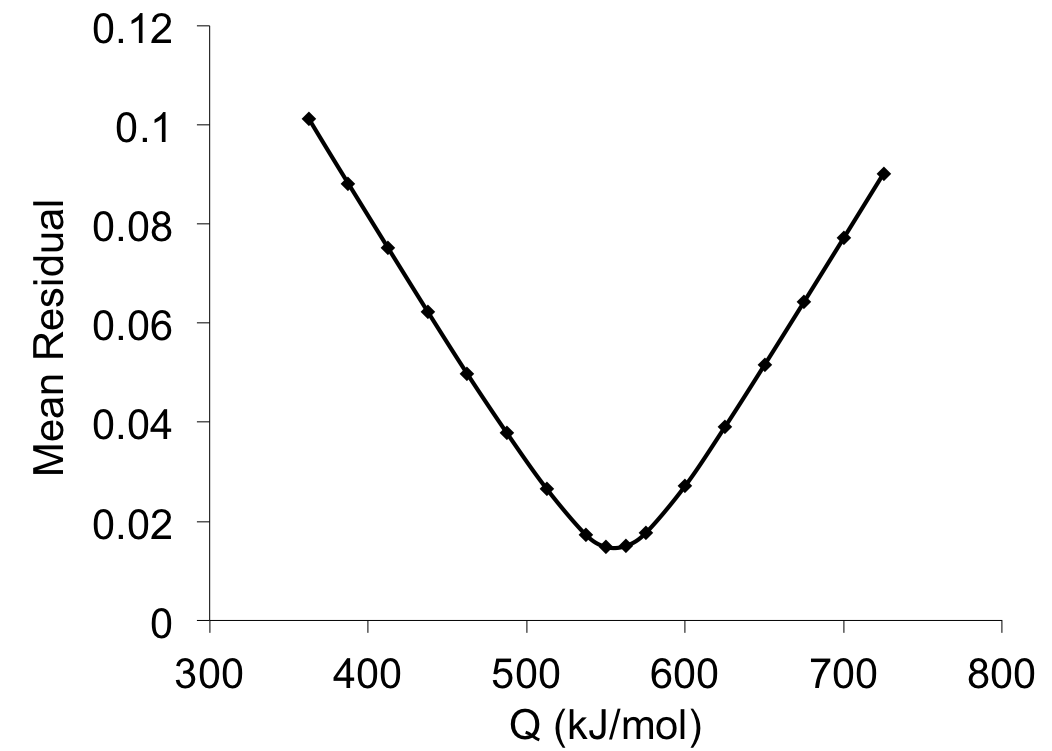
\includegraphics[width=\textwidth]{Chapter-6/Figures/Figure4.png}
	\caption{Mean residuals of the MSCs assuming different values for $Q$ for non-aqueous slip cast CT3000 LS SG samples.}
	\label{Ch6-figure:Figure4}
\end{figure}
%%%

\newpage
%%%
\begin{figure}[H]
	\centering
	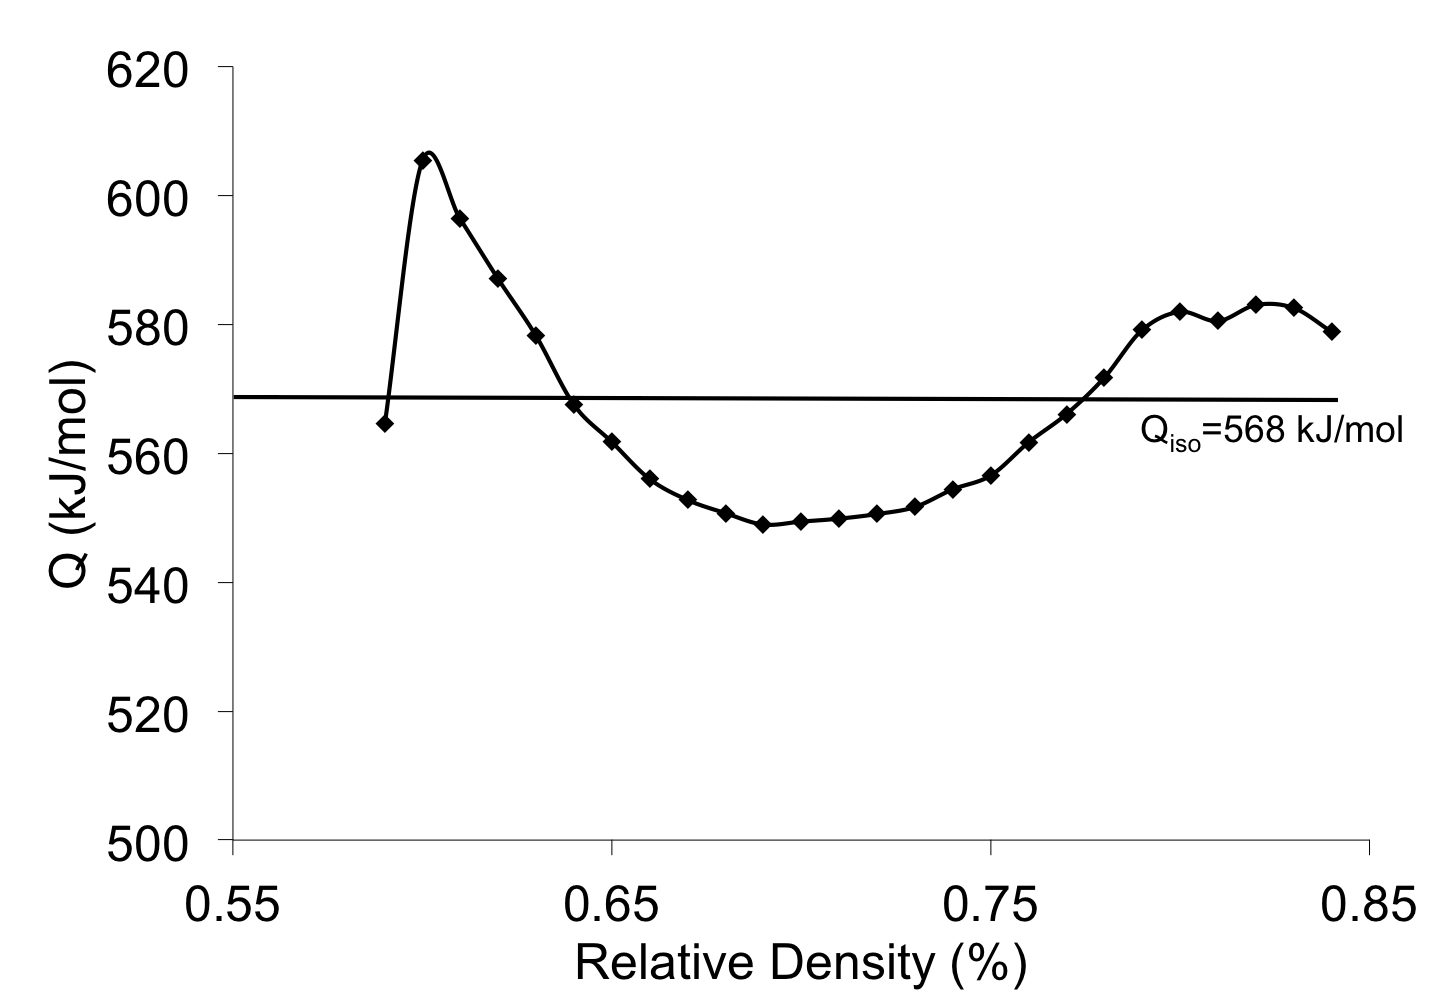
\includegraphics[width=\textwidth]{Chapter-6/Figures/Figure5.png}
	\caption{MSCs of CT3000 LS SG samples prepared by non-aqueous slip casting using a) the $Q$-value obtained by accounting for shrinkage anisotropy ($Q$=550 kJ/mol) and b) using $Q$-value when shrinkage anisotropy was uncorrected for ($Q$ = 625 kJ/mol).}
	\label{Ch6-figure:Figure5}
\end{figure}
%%%

\newpage
%%%
\begin{figure}[H]
	\centering
	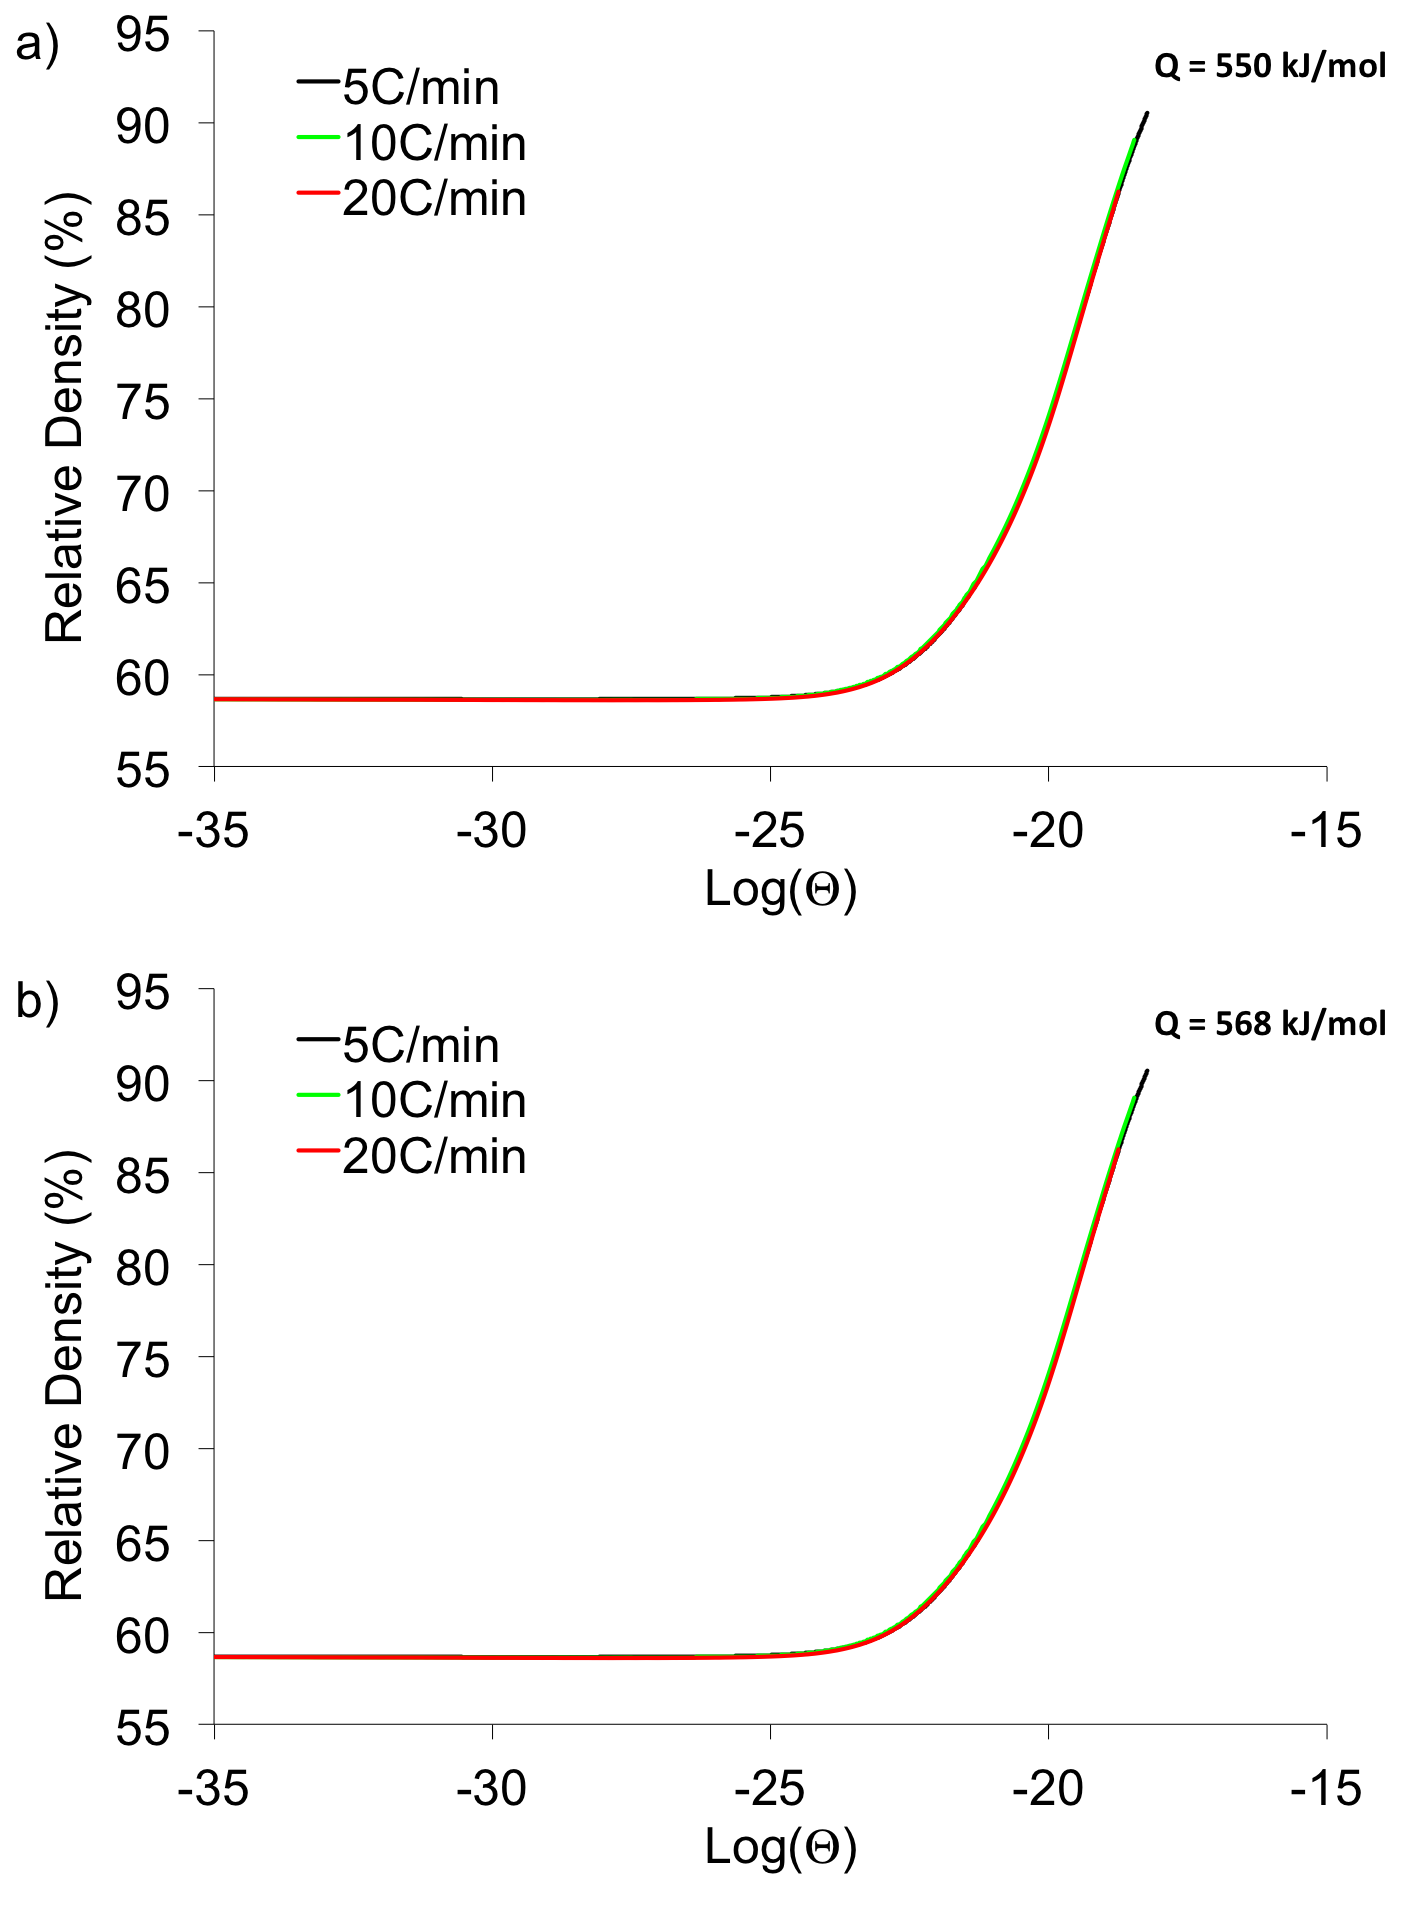
\includegraphics[width=\textwidth]{Chapter-6/Figures/Figure6.png}
	\caption{MSCs and $Q$-values of CT3000LS-SG samples obtained from the minimum mean residuals for samples prepared by different forming techniques and accounting for shrinkage anisotropy.}
	\label{Ch6-figure:Figure6}
\end{figure}
%%%

\newpage
%%%
\begin{figure}[H]
	\centering
	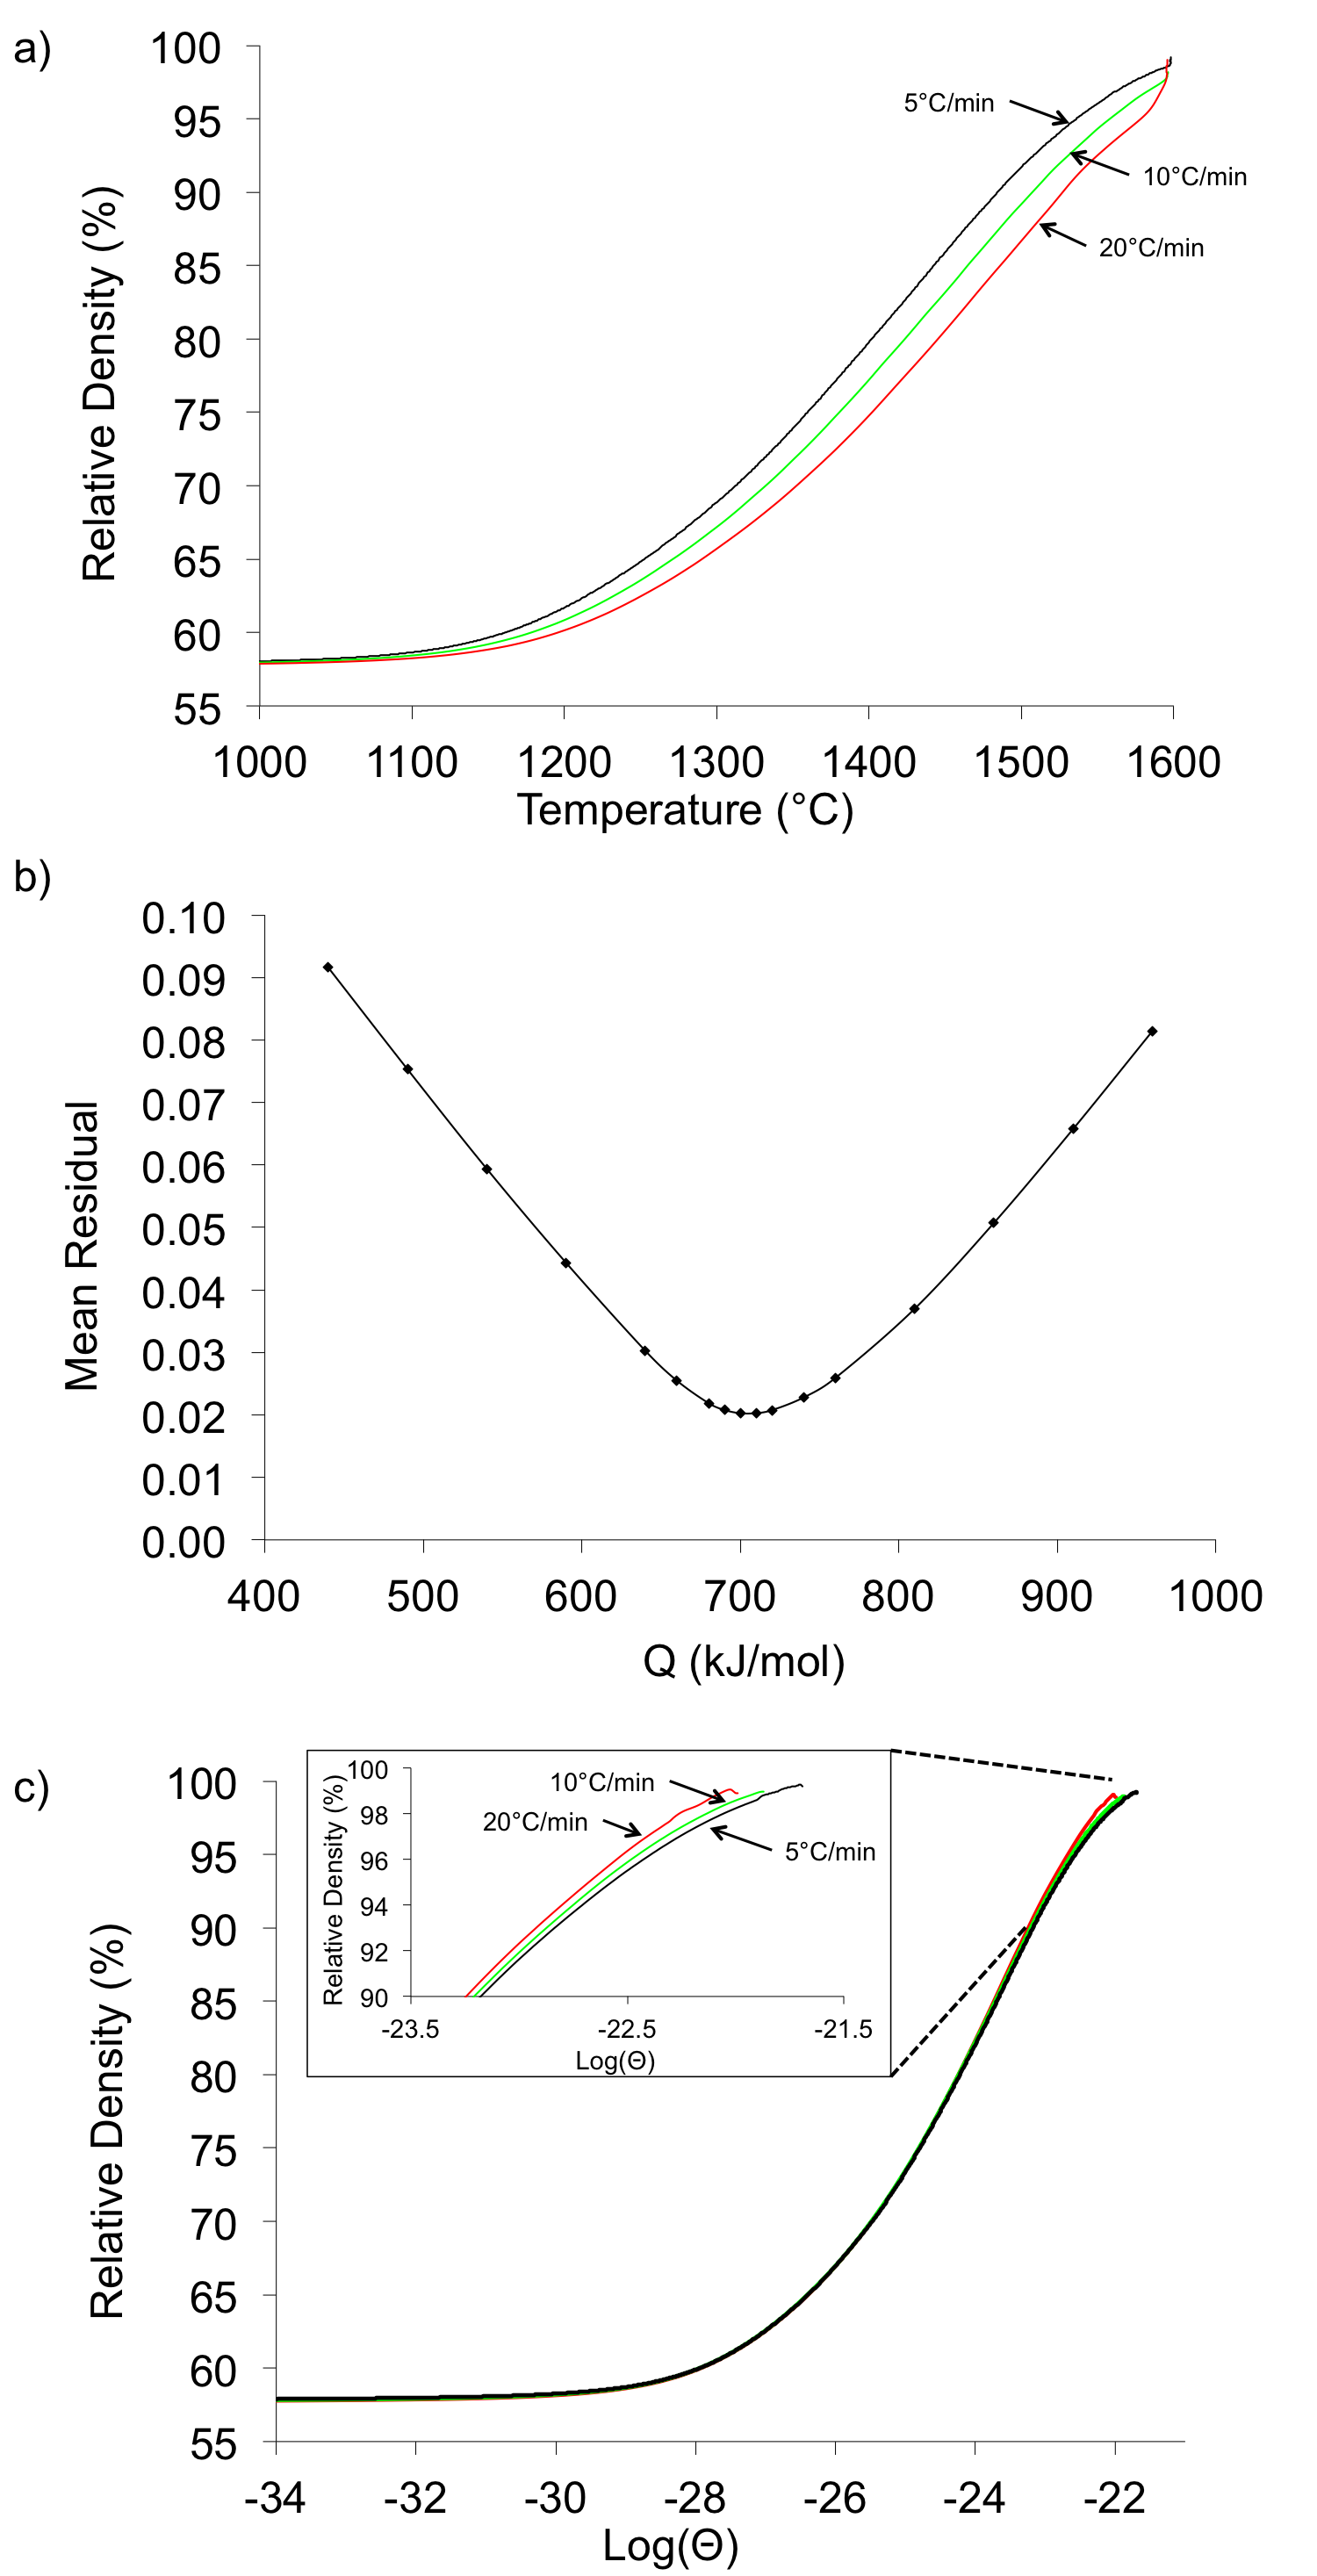
\includegraphics[scale=0.4]{Chapter-6/Figures/Figure7.png}
	\caption{a) Densification of dry pressed CT3000 LS SG samples at different heating rates, b) mean residuals as a function of $Q$, and c) MSC for $Q$ = 700 kJ/mol obtained from the minimum mean residuals, showing divergence at densities >90\%.}
	\label{Ch6-figure:Figure7}
\end{figure}
%%%

\newpage
%%%
\begin{figure}[H]
	\centering
	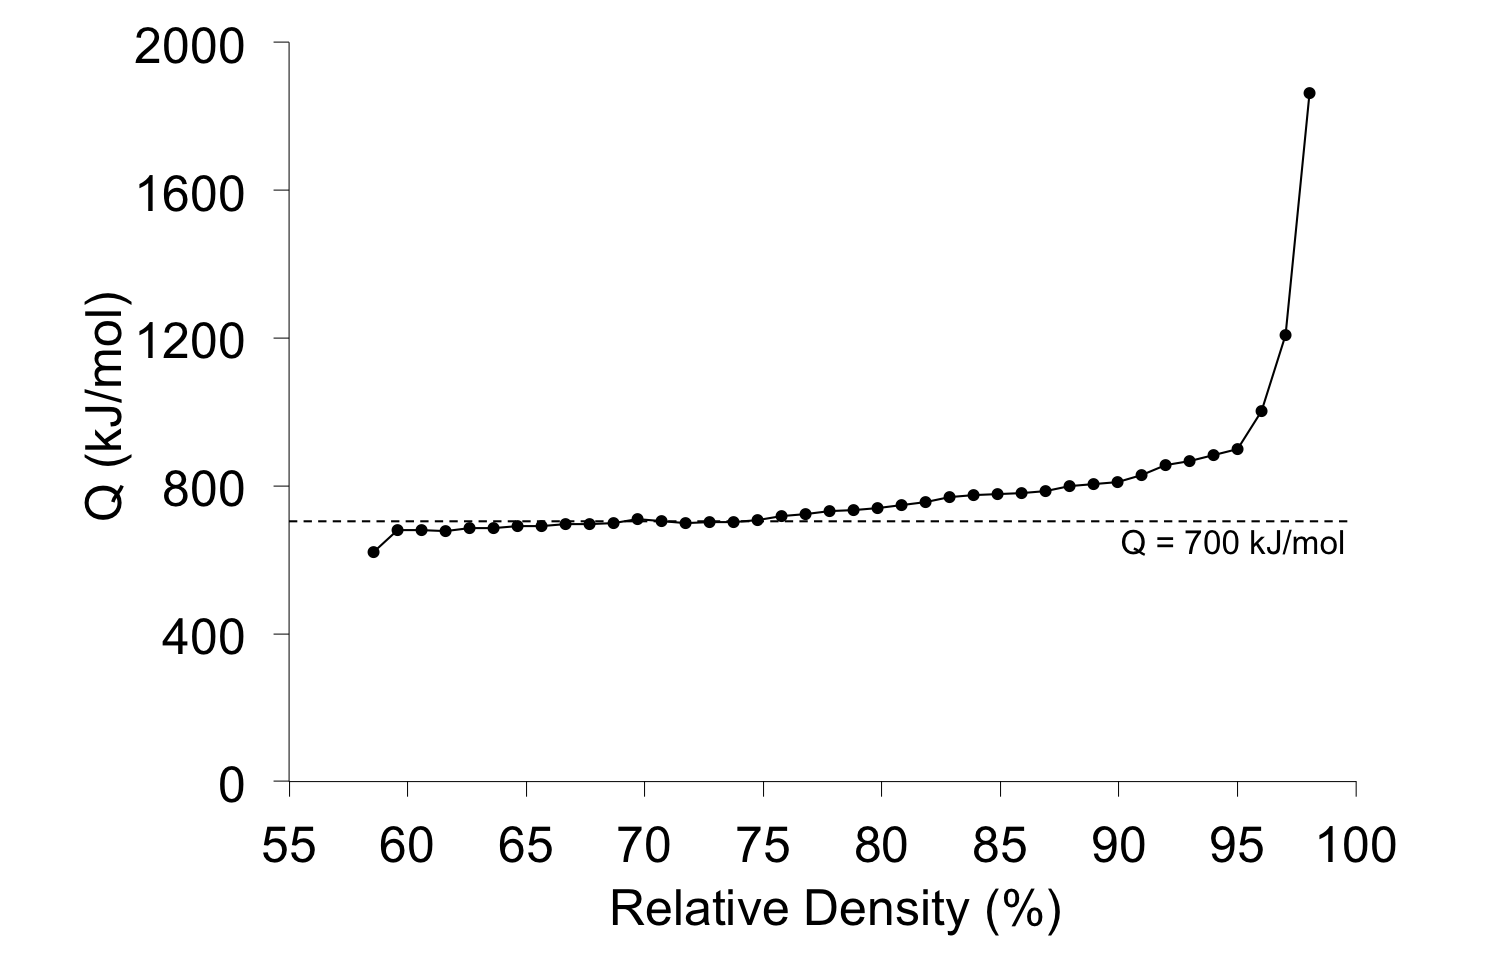
\includegraphics[width=\textwidth]{Chapter-6/Figures/Figure8.png}
	\caption{$Q$-values for dry pressed CT3000 LS SG samples as a function of relative density obtained from iso-density analysis.}
	\label{Ch6-figure:Figure8}
\end{figure}
%%%

\newpage
%%%
\begin{figure}[H]
	\centering
	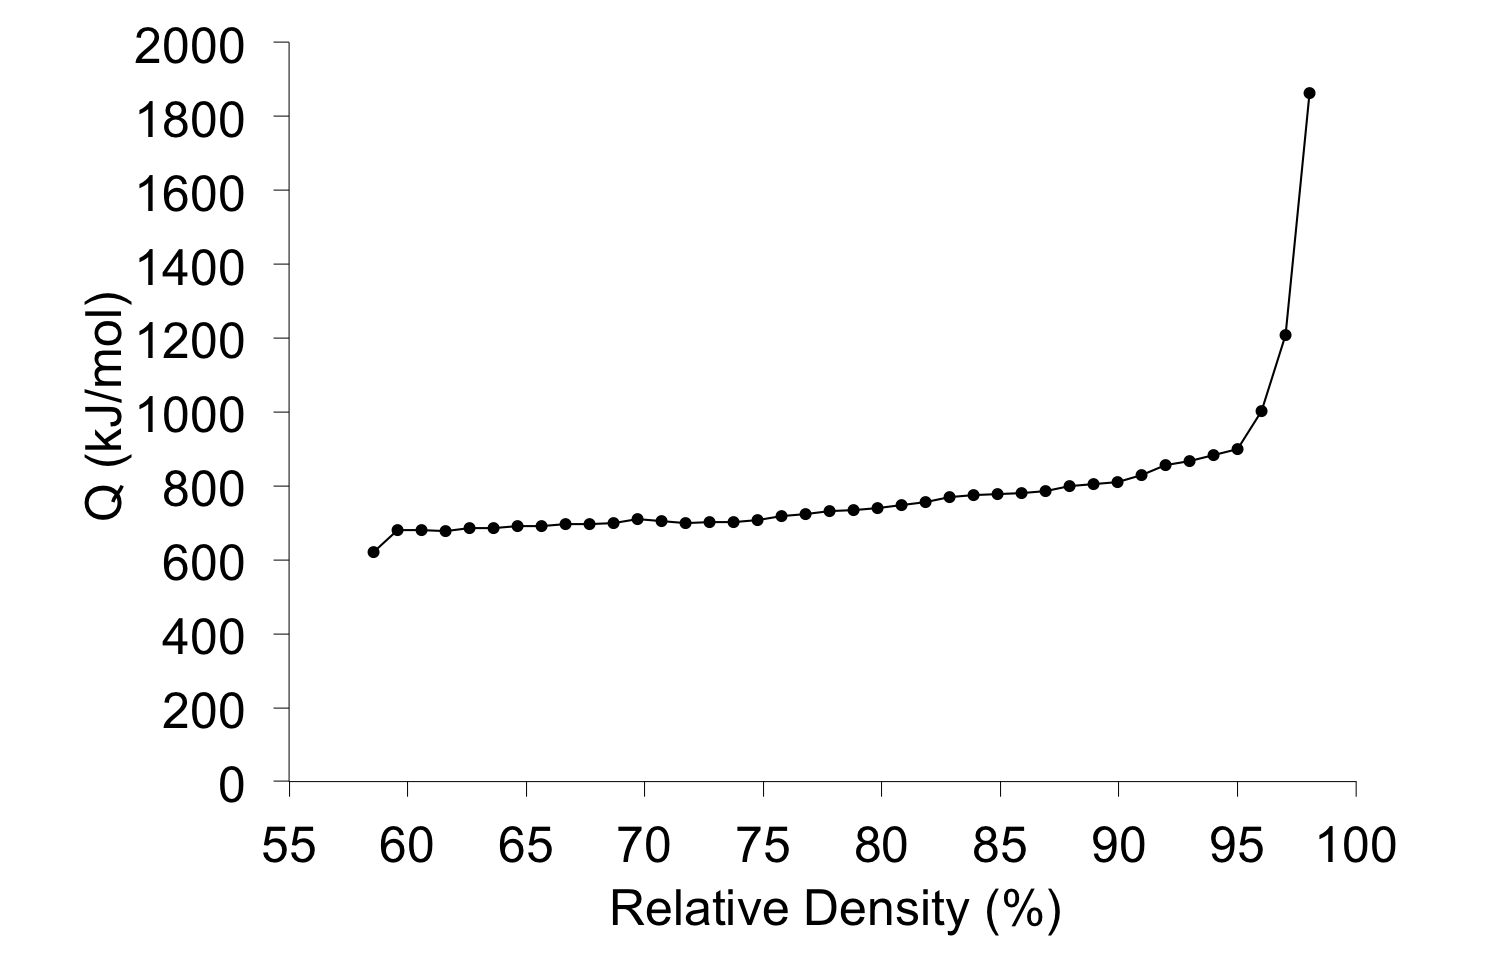
\includegraphics[width=\textwidth]{Chapter-6/Figures/Figure9.png}
	\caption{Development of the microstructural parameters, summarized in the $C$ parameter, as a function of relative density for dry pressed CT3000 LS SG samples.}
	\label{Ch6-figure:Figure9}
\end{figure}
%%%

\newpage
%%%
\begin{figure}[H]
	\centering
	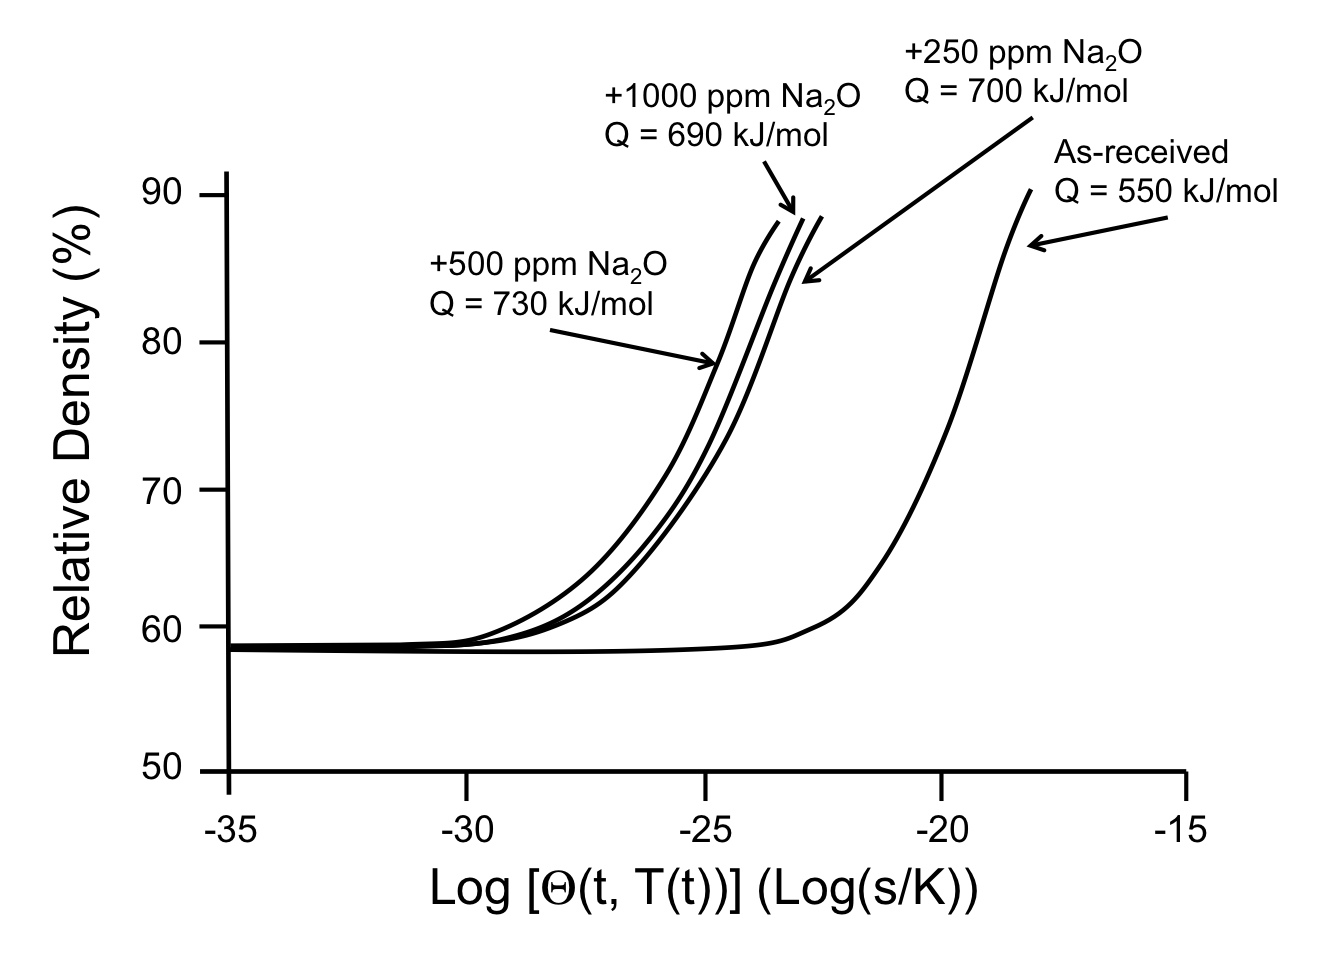
\includegraphics[width=\textwidth]{Chapter-6/Figures/Figure10.png}
	\caption{MSCs and $Q$-values for CT3000 LS SG samples prepared by non-aqueous slip casting with different Na$_{2}$O concentrations.}
	\label{Ch6-figure:Figure10}
\end{figure}
%%%

\newpage
%%%
\begin{figure}[H]
	\centering
	\includegraphics[width=\textwidth]{Chapter-6/Figures/Figure11.png}
	\caption{Equivalent time/temperature diagram for CT3000 LS SG samples prepared by non-aqueous slip casting heated at 10$^{\circ}$C/min. The contours may be used to predict heat treatments requirements to achieve a desired density.}
	\label{Ch6-figure:Figure11}
\end{figure}
%%%

\chapter{Summary and Future Work}

\section{Introduction}
When in the Course of human events, it becomes necessary for one people  to dissolve the political bands which have connected them with another,  and to assume among the powers of the earth, the separate and equal station  to which the Laws of Nature and of Nature's God entitle them, a decent respect to the opinions of mankind requires that they should declare  the causes which impel them to the separation.

\section{More Declaration}

We hold these truths to be self-evident, that all men are created equal,  that they are endowed by their Creator with certain unalienable Rights,  that among these are Life, Liberty and the pursuit of Happiness. --That to secure these  rights, Governments are instituted among Men, deriving their just powers  from the consent of the governed, --That whenever any Form of Government  becomes destructive of these ends, it is the Right of the People to alter  or to abolish it, and to institute new Government, laying its foundation on  such principles and organizing its powers in such form, as to them shall  seem most likely to effect their Safety and Happiness. Prudence, indeed, will dictate that Governments long established should not  be changed for light and transient causes; and accordingly all experience  hath shewn, that mankind are more disposed to suffer, while evils are  sufferable, than to right themselves by abolishing the forms to which they  are accustomed. But when a long train of abuses and usurpations, pursuing invariably the same  Object evinces a design to reduce them under absolute Despotism, it is their  right, it is their duty, to throw off such Government, and to provide new Guards for their future security. --Such has been the patient sufferance of these Colonies; and such is now the  necessity which constrains them to alter their former Systems of Government.  The history of the present King of Great Britain [George III] is a history  of repeated injuries and usurpations, all having in direct object the  establishment of an absolute Tyranny over these States. To prove this, let Facts be submitted to a candid world.
%%%%%%%%%%%%%%%%%%%%%%%%%%%%%%%%%%%%%%%%%%%%%%%%%%%%%%%%%%%%%%%
% Appendices
%
% Because of a quirk in LaTeX (see p. 48 of The LaTeX
% Companion, 2e), you cannot use \include along with
% \addtocontents if you want things to appear the proper
% sequence.
%%%%%%%%%%%%%%%%%%%%%%%%%%%%%%%%%%%%%%%%%%%%%%%%%%%%%%%%%%%%%%%
\appendix
\titleformat{\chapter}[display]{\fontsize{30}{30}\selectfont\bfseries\sffamily}{Appendix \thechapter\textcolor{gray75}{\raisebox{3pt}{|}}}{0pt}{}{}
% If you have a single appendix, then to prevent LaTeX from
% calling it ``Appendix A'', you should uncomment the following two
% lines that redefine the \thechapter and \thesection:
%\renewcommand\thechapter{}
%\renewcommand\thesection{\arabic{section}}
%\Appendix{Title of the First Appendix}

\section{Introduction}
When in the Course of human events, it becomes necessary for one people  to dissolve the political bands which have connected them with another,  and to assume among the powers of the earth, the separate and equal station  to which the Laws of Nature and of Nature's God entitle them, a decent respect to the opinions of mankind requires that they should declare  the causes which impel them to the separation.

\section{More Declaration}

We hold these truths to be self-evident, that all men are created equal,  that they are endowed by their Creator with certain unalienable Rights,  that among these are Life, Liberty and the pursuit of Happiness. --That to secure these  rights, Governments are instituted among Men, deriving their just powers  from the consent of the governed, --That whenever any Form of Government  becomes destructive of these ends, it is the Right of the People to alter  or to abolish it, and to institute new Government, laying its foundation on  such principles and organizing its powers in such form, as to them shall  seem most likely to effect their Safety and Happiness.

\subsection{Some Subsection Title Here}

Prudence, indeed, will dictate that Governments long established should not  be changed for light and transient causes; and accordingly all experience  hath shewn, that mankind are more disposed to suffer, while evils are  sufferable, than to right themselves by abolishing the forms to which they  are accustomed. But when a long train of abuses and usurpations, pursuing invariably the same  Object evinces a design to reduce them under absolute Despotism, it is their  right, it is their duty, to throw off such Government, and to provide new Guards for their future security. --Such has been the patient sufferance of these Colonies; and such is now the  necessity which constrains them to alter their former Systems of Government.  The history of the present King of Great Britain [George III] is a history  of repeated injuries and usurpations, all having in direct object the  establishment of an absolute Tyranny over these States. To prove this, let Facts be submitted to a candid world.
%\Appendix{Title of the Second Appendix}

\section{Introduction}
When in the Course of human events, it becomes necessary for one people  to dissolve the political bands which have connected them with another,  and to assume among the powers of the earth, the separate and equal station  to which the Laws of Nature and of Nature's God entitle them, a decent respect to the opinions of mankind requires that they should declare  the causes which impel them to the separation.

\section{More Declaration}

We hold these truths to be self-evident, that all men are created equal,  that they are endowed by their Creator with certain unalienable Rights,  that among these are Life, Liberty and the pursuit of Happiness. --That to secure these  rights, Governments are instituted among Men, deriving their just powers  from the consent of the governed, --That whenever any Form of Government  becomes destructive of these ends, it is the Right of the People to alter  or to abolish it, and to institute new Government, laying its foundation on  such principles and organizing its powers in such form, as to them shall  seem most likely to effect their Safety and Happiness. Prudence, indeed, will dictate that Governments long established should not  be changed for light and transient causes; and accordingly all experience  hath shewn, that mankind are more disposed to suffer, while evils are  sufferable, than to right themselves by abolishing the forms to which they  are accustomed. But when a long train of abuses and usurpations, pursuing invariably the same  Object evinces a design to reduce them under absolute Despotism, it is their  right, it is their duty, to throw off such Government, and to provide new Guards for their future security. --Such has been the patient sufferance of these Colonies; and such is now the  necessity which constrains them to alter their former Systems of Government.  The history of the present King of Great Britain [George III] is a history  of repeated injuries and usurpations, all having in direct object the  establishment of an absolute Tyranny over these States. To prove this, let Facts be submitted to a candid world.
%\Appendix{Title of the Third Appendix}

\section{Introduction}
When in the Course of human events, it becomes necessary for one people  to dissolve the political bands which have connected them with another,  and to assume among the powers of the earth, the separate and equal station  to which the Laws of Nature and of Nature's God entitle them, a decent respect to the opinions of mankind requires that they should declare  the causes which impel them to the separation.

\section{More Declaration}

We hold these truths to be self-evident, that all men are created equal,  that they are endowed by their Creator with certain unalienable Rights,  that among these are Life, Liberty and the pursuit of Happiness. --That to secure these  rights, Governments are instituted among Men, deriving their just powers  from the consent of the governed, --That whenever any Form of Government  becomes destructive of these ends, it is the Right of the People to alter  or to abolish it, and to institute new Government, laying its foundation on  such principles and organizing its powers in such form, as to them shall  seem most likely to effect their Safety and Happiness. Prudence, indeed, will dictate that Governments long established should not  be changed for light and transient causes; and accordingly all experience  hath shewn, that mankind are more disposed to suffer, while evils are  sufferable, than to right themselves by abolishing the forms to which they  are accustomed. But when a long train of abuses and usurpations, pursuing invariably the same  Object evinces a design to reduce them under absolute Despotism, it is their  right, it is their duty, to throw off such Government, and to provide new Guards for their future security. --Such has been the patient sufferance of these Colonies; and such is now the  necessity which constrains them to alter their former Systems of Government.  The history of the present King of Great Britain [George III] is a history  of repeated injuries and usurpations, all having in direct object the  establishment of an absolute Tyranny over these States. To prove this, let Facts be submitted to a candid world.
%\Appendix{Title of the Fourth Appendix}

\section{Introduction}
When in the Course of human events, it becomes necessary for one people  to dissolve the political bands which have connected them with another,  and to assume among the powers of the earth, the separate and equal station  to which the Laws of Nature and of Nature's God entitle them, a decent respect to the opinions of mankind requires that they should declare  the causes which impel them to the separation.

\section{More Declaration}

We hold these truths to be self-evident, that all men are created equal,  that they are endowed by their Creator with certain unalienable Rights,  that among these are Life, Liberty and the pursuit of Happiness. --That to secure these  rights, Governments are instituted among Men, deriving their just powers  from the consent of the governed, --That whenever any Form of Government  becomes destructive of these ends, it is the Right of the People to alter  or to abolish it, and to institute new Government, laying its foundation on  such principles and organizing its powers in such form, as to them shall  seem most likely to effect their Safety and Happiness. Prudence, indeed, will dictate that Governments long established should not  be changed for light and transient causes; and accordingly all experience  hath shewn, that mankind are more disposed to suffer, while evils are  sufferable, than to right themselves by abolishing the forms to which they  are accustomed. But when a long train of abuses and usurpations, pursuing invariably the same  Object evinces a design to reduce them under absolute Despotism, it is their  right, it is their duty, to throw off such Government, and to provide new Guards for their future security. --Such has been the patient sufferance of these Colonies; and such is now the  necessity which constrains them to alter their former Systems of Government.  The history of the present King of Great Britain [George III] is a history  of repeated injuries and usurpations, all having in direct object the  establishment of an absolute Tyranny over these States. To prove this, let Facts be submitted to a candid world.
%\Appendix{Title of the Fifth Appendix}

\section{Introduction}
When in the Course of human events, it becomes necessary for one people  to dissolve the political bands which have connected them with another,  and to assume among the powers of the earth, the separate and equal station  to which the Laws of Nature and of Nature's God entitle them, a decent respect to the opinions of mankind requires that they should declare  the causes which impel them to the separation.

\pagebreak
Some text.
{\lstset{language=Fortran}
\footnotesize
\begin{lstlisting}
      program chaos
c When a LS Fortran program has been compiled and linked into Mac
c application, all information written to the screen WRITE(6,...) or
c WRITE(*,...) appears in a standard Mac window, complete with basic
c menus.
      external fex, jac
      double precision atol, rtol, rwork, t, tout, h
      double precision ttotal, dtout
      dimension h(3), atol(3), rwork(70), iwork(23)
	  character*8 tstart, tend
      neq = 3
	  
	  call time(tstart)
	  write(6,*) "begin integration at  ", tstart
      write(6,*)
	  
c --- Read in the total initial angular momentum.  The total angular
c     momentum H is always unity due to normalization.
	  open(unit = 2, file = 'chaos.data', status = 'unknown')
      read(2,*) h(1), h(2), h(3)
	  
c --- The integration begins at t = 0 and the values are printed at
c     every tout.  tout is incremented below.  ttotal is the length
c     of the entire integration.  The number of recorded values of
c     the integration is given by npoints.
      t = 0.0d0
      tout = 0.0d0
      write(6,*) 'Duration of integration interval, i.e., tfinal?'
      read(6,*) ttotal
      write(6,*)
      write(6,*) 'Number of points for trajectory plot?'
      read(6,*) npoints
      write(6,*)
      dtout = ttotal/dfloat(npoints)
      tout = tout + dtout
	  
c --- Tolerance parameters used by lsoda.
      itol = 2
      rtol = 1.0d-9
      atol(1) = 1.0d-9
      atol(2) = 1.0d-9
      atol(3) = 1.0d-9
	  
c --- Other parameters used by lsoda.  See below.
      itask = 1
      istate = 1
      iopt = 1
      lrw = 70
      liw = 23
      jt = 1

      do 11 kount = 5,10
         rwork(kount) = 0.0d0
         iwork(kount) = 0
  11  continue
      iwork(6) = 100000
	  
	  open(unit = 3, file = 'traj.dat', disp = 'keep',
     &     status = 'unknown')
	 
c --- The actual integration begins here.  Loop on the value of iout.
      do 40 iout = 1, npoints
	  
         call lsoda(fex,neq,h,t,tout,itol,rtol,atol,itask,istate,
     &              iopt,rwork,lrw,iwork,liw,jdum,jt)
	  
c ------ Write the output to the file traj.dat.
         write(3,20) t, h(1), h(2), h(3)
  20     format(f9.1, 3e15.6)

         if (mod(tout,5000.0d0) .eq. 0.0d0) then
            write(6,*) tout
         end if
  
c ------ Check to see that things are going OK.
         if (istate .lt. 0) go to 80
		 
c ------ Set the time at which the integration is next recorded and
c        continue the do-loop.
  40     tout = tout + dtout
  
      write(6,*) 'number of steps taken: ', iwork(11)
      write(6,*) 'number of f evaluations: ', iwork(12)
      write(6,*) 'number of Jacobian evaluations: ', iwork(13)
      write(6,*) 'method order last used: ', iwork(14)
      write(6,*) 'method last used (2 = stiff): ', iwork(19)
      write(6,*) 'value of t at last method switch: ', rwork(15)
      write(6,*)
	 
	  call time(tend)
	  write(6,*) "end integration at  ", tend
      stop
	  
c --- If there is an error, given by istate < 0, write the following.
  80  write(6,90) istate
  90  format(///22h error halt.. istate =,i3)
  
      stop
      end

\end{lstlisting}
}

%%%%%%%%%%%%%%%%%%%%%%%%%%%%%%%%%%%%%%%%%%%%%%%%%%%%%%%%%%%%%%%
% ESM students need to include a Nontechnical Abstract as the %
% last appendix.                                              %
%%%%%%%%%%%%%%%%%%%%%%%%%%%%%%%%%%%%%%%%%%%%%%%%%%%%%%%%%%%%%%%
% This \include command should point to the file containing
% that abstract.
%\include{nontechnical-abstract}
%%%%%%%%%%%%%%%%%%%%%%%%%%%%%%%%%%%%%%%%%%%
} % End of the \allowdisplaybreak command %
%%%%%%%%%%%%%%%%%%%%%%%%%%%%%%%%%%%%%%%%%%%

%%%%%%%%%%%%%%%%
% BIBLIOGRAPHY %
%%%%%%%%%%%%%%%%
% You can use BibTeX or other bibliography facility for your
% bibliography. LaTeX's standard stuff is shown below. If you
% bibtex, then this section should look something like:
	\begin{singlespace}
	\bibliographystyle{GLG-bibstyle}
	\addcontentsline{toc}{chapter}{Bibliography}
	\bibliography{Biblio-Database}
	\end{singlespace}

%\begin{singlespace}
%\begin{thebibliography}{99}
%\addcontentsline{toc}{chapter}{Bibliography}
%\frenchspacing

%\bibitem{Wisdom87} J. Wisdom, ``Rotational Dynamics of Irregularly Shaped Natural Satellites,'' \emph{The Astronomical Journal}, Vol.~94, No.~5, 1987  pp. 1350--1360.

%\bibitem{G&H83} J. Guckenheimer and P. Holmes, \emph{Nonlinear Oscillations, Dynamical Systems, and Bifurcations of Vector Fields}, Springer-Verlag, New York, 1983.

%\end{thebibliography}
%\end{singlespace}

\backmatter

% Vita
\vita{SupplementaryMaterial/Vita}

\end{document}

